


\documentclass[12pt]{article}
\def\myfont{\fontfamily{cmss}\selectfont}

\usepackage{fancyhdr, amsmath, amssymb, amsfonts, url, subfigure, dsfont, mathrs
fs, graphicx, epsfig, subfigure, amsthm, manfnt, tikz}
\usepackage{cmbright}
\usepackage[T1]{fontenc}
\usepackage{enumerate}
\usepackage{bm}
%\bibliographystyle{plain}
%\usepackage[sort&compress]{natbib}
%\bibpunct{[}{]}{,}{a}{,}{,}
\setlength{\textwidth}{6.5 in}
\setlength{\oddsidemargin}{0 in}


%%%%%%%%hyperlinked contents
\usepackage{color}   %May be necessary if you want to color links
\usepackage{hyperref}
\hypersetup{
    colorlinks=true, %set true if you want colored links
    linktoc=all,     %set to all if you want both sections and subsections linked
    linkcolor=blue,  %choose some color if you want links to stand out
}
%%%%%%%%%


\newlength{\guillotine}
\setlength{\guillotine}{-\headheight}
\addtolength{\guillotine}{-\headsep}
\setlength{\topmargin}{\guillotine}
\setlength{\textheight}{9 in}

\pagestyle{fancyplain}
\renewcommand{\headrulewidth}{.5pt}
\renewcommand{\footrulewidth}{.5pt}
\newtheorem{theorem}{Theorem}[section]
\newtheorem{corollary}[theorem]{Corollary}
\newtheorem{lemma}[theorem]{Lemma}
\newtheorem{proposition}[theorem]{Proposition}
\newtheorem{sketch}[theorem]{Sketch of Proof}
\newtheorem{question}[theorem]{Question}
\newtheorem{conj}[theorem]{Conjecture}

\theoremstyle{definition}
\newtheorem{definition}[theorem]{Definition}
\newtheorem{example}[theorem]{Example}
\newtheorem{examples}[theorem]{Examples}
\theoremstyle{remark}
\newtheorem{remark}[theorem]{Remark}
\newtheorem{remarks}[theorem]{Remarks}
\newtheorem{exercise}[theorem]{Exercise}
%\newtheoremstyle{example}


\date{}









\begin{document}
\bibliographystyle{plain} 
\title{MA424 Dynamical Systems \\ Course Notes (2025-26)}% \lebn]
%{MAS427 Ergodic Theory} 

\author{Lecturer: Han Yu} 




%\thanks{}

%\keywords{spectral triple, Dixmier trace, conformal graph directed Markov 
%system, conformal measure, Patterson-Sullivan measure}

%\date{\today}

%\begin{abstract}
%For conformal graph directed Markov systems, we construct a spectral triple
%from which one can recover the associated conformal measure via
%a Dixmier trace. As a particular case, we can recover 
%the Patterson-Sullivan
%measure for a class of Kleinian groups.
%\end{abstract}

\maketitle

\tableofcontents

\newpage

%\lecture{1}{Introduction and Uniform Distribution}

%\myfont
%\myfont{
\setcounter{section}{-1}
\section{Introductory Remarks}
This version of the notes is based on the materials prepared by Han Yu for 2025-26, largely derived
 from earlier sets of MA424 lecture notes by Stephen Cantrell, Vassili Gelfreich, Mark Pollicott and Richard Sharp,
with some reordering, deletions and additions. Some material, particularly on topological
dynamics, is based on 
Peter Walters' book \cite{Walters}.

Other introductions to the theory of dynamical systems are provided by the books
\cite{BS02}, \cite{Dev03}, \cite{HK03} and \cite{Ste10}. 
Introductory texts on complex dynamics (section 6)
are  \cite{Bea91} and \cite{Stein93}.
An encyclopaedic treatment of the theory is given by Katok and Hasselblatt in the monumental \cite{KH95} (800 pages).

Put loosely, the aim of the module is to scratch the surface of understanding the behaviour 
of iterates of a continuous map $f : X \to X$, where $X$ is a compact metrisable space,
sometimes with more stringent conditions being imposed (e.g. that $X$ is a manifold
and that $f$ is differentiable of some order). One might also consider continuous time dynamics,
known as flows, where one has a continuous mapping $F : X \times \mathbb R \to X$
such that $f^t(x) := F(x,t)$ (to use customary notation)
satisfies
$f^0 = \mathrm{id}$ (the identity map) and $f^{s+t} = f^s \circ f^t$. However, we will not have time to consider such systems.

As a subject, dynamical systems may be said to have begun with the work of Poincar\'e
on celestial mechanics and, in particular, on the three body problem. Indeed, it was Poincar\'e's discovery of a mistake in his own work on this problem that led him to discover the essential mechanism giving rise to chaotic behaviour, later rediscovered and simplified by Smale in the 1960s. It was also due to Poincar\'e that circle homeomorphisms became important objects of study,
as they arose in his attempt to classify flows on the two-dimensional torus.
Celestial mechanics also led to the so-called KAM theory developed by Kolmogorov, Arnold and Moser in the mid-20th century -- another important topic that we will not have time to discuss.
Instead, we shall switch our attention to expanding map,
which provide an easy introduction to the theory of hyperbolic systems, which, while studied earlier in the work of Hadamard at the end of the 19th century,
and Artin, Hedlund, Hopf and Morse from the 1920s onwards, became a well-defined
area due to the impetus of the work of Anosov \cite{Anosov67} and Smale \cite{Smale67} in the 1960s.
This topic is further developed in the module MA4N3 Hyperbolic Dynamics.


The module naturally pairs with MA427 Ergodic Theory and they may be taken in either order.
In ergodic theory one studies that situation where the map $f$ preserves a measure and one wants to understand typical behaviour with respect to that measure. This has its roots in statistical mechanics and the work of Boltzmann. Boltzmann's ``ergodic hypothesis'', that time averages are equal to space averages, is clearly incorrect as a general statement but led to the ergodic theorems
of Birkhoff and von Neumann in the 1930s, which deal with 
convergence of time averages almost everywhere (in the sense of measure theory) and in $L^2$,
respectively.
There is cross-fertilization between this and the topological point of view. For example, 
topological transitivity should be seen as analogous to ergodicity and
minimality should 
be
seen as analogous to unique ergodicity -- and there are rather more obvious parallels between the notions of mixing that appear in the two subjects.

%the introduction of entropy as an
%invariant in ergodic theory in the 1950s inspired the definition of topological entropy which we'll see %later.

%Previously, there was a section 6 -- which I never managed to cover -- on complex dynamics. However,
%there is now an excellent new module MA4M7 Complex Dynamics running this term. 
%I hope there will be some synergy for students who take both (not necessarily at the same time) but
%they are formally independent.


\newpage

\section{Topological Dynamics}

This module will primarily concern the dynamics of a single continuous transformation 
$f : X \to X$ on a topological space
$X$. 
While many definitions make sense in this general setting, we will assume that
$X$ is metrizable. Sometimes we will need to work with a fixed metric on $X$.
For the most part, $X$ will be compact (or we will concentrate on an interesting compact subset of $X$).
Whether or not $f$ is invertible will often play a role. Recall that $f$ is called a homeomorphism if 
it is invertible (i.e. a bijection) and
both $f$ and $f^{-1}$ are continuous. 


Sometimes, $f$ will have greater regularity than continuity. However, 
the general theory in this section will be developed for continuous transformations.

{\it Throughout this section, unless stated otherwise, $X$ is a compact metrizable space 
%(with a metric $d$)
and $f : X \to X$ is a continuous
transformation.}

\subsection{A little set theory}

Let $X$ and $Y$ be sets and let $f : X \to Y$ be a function. (Nothing more is assumed for the moment.)
Even if $f$ is not invertible, for $A \subset Y$ we define
\[
f^{-1}(A) = \{x \in X \hbox{ : } f(x) \in A\}.
\]
For $y \in Y$, we write
\[
f^{-1}(y) := f^{-1}(\{y\}) =\{x \in X \hbox{ : } f(x)=y\}.
\]
If $f$ is invertible, then we interpret $f^{-1}(y)$ as a point (the image of $y$ under the map $f^{-1}$)
but this should not cause confusion.

It is worth recalling the following identities.
If $f : X \to Y$ is a function and $\{A_\alpha\}$ is an arbitrary collection of subsets of $Y$
then
\[
f^{-1}\left(\bigcup_\alpha A_\alpha\right) 
= \bigcup_\alpha f^{-1}(A_\alpha)
\quad \text{and} \quad
f^{-1}\left(\bigcap_\alpha A_\alpha\right) 
= \bigcap_\alpha f^{-1}(A_\alpha).
\]
Furthermore, if $f$ is invertible then 
\[
f\left(\bigcup_\alpha A_\alpha\right) 
= \bigcup_\alpha f(A_\alpha)
\quad \text{and} \quad
f\left(\bigcap_\alpha A_\alpha\right) 
= \bigcap_\alpha f(A_\alpha).
\]
%(This only requires $X$ to be a set and $f:X\to X$ a function.)

\subsection{Orbits}

Let $X$ be a compact metrizable topological space and $f: X \to X$ be a continuous map. 
We will call the pair $(X,f)$ a {\it dynamical system}.
For $x \in X$, we say that its {\it orbit} 
(or {\it forward orbit}) is
\[
x, fx, f^2x ,\ldots, f^nx ,\ldots
\]
(where $f^2 = f \circ f$, etc.).
If $f$ is invertible then we might also consider the two-sided orbit
\[
\ldots f^{-n}x ,\ldots ,f^{-2}x,f^{-1}x,x,fx,f^2x,\ldots,f^nx,\ldots;
\]
and we will make clear which we mean. We write
\[
\mathcal O_f^+(x) = \{f^n x \hbox{ : } n\in \mathbb Z^+\}
\]
and 
\[
\mathcal O_f(x) = \{f^n x \hbox{ : } n\in \mathbb Z\}.
\]

If $fx=x$ we say that $x$ is a {\it fixed point} of $f$. If $f^nx=x$ for some $n \ge 1$ we say that 
$x$ is a {\it periodic point} of period $n$. If there is no $1 \le m <n$ such that
$f^mx=x$ then we call $n$ the {\it least period} or prime period. We also refer to
\[
x,fx, \ldots, f^{n-1}x
\]
as a {\it periodic orbit} (or as a {\it prime periodic orbit} when $n$ is the least period).

At the opposite extreme to periodic orbits are dense orbits. There are examples of dynamical systems for which all orbits are dense, i.e. for all $x \in X$, $\mathcal O^+_f(x)$ is dense in $X$. On the other hand, we may well have a mixture of periodic orbits, dense orbits and orbits which are neither periodic nor dense.
Examples of all these situations will appear below.

%For $x \in X$, we define $\omega_T(x)$, called the $\omega$-limit set of $x$, to be the set of limit points of
%the orbit of $x$.

\subsection{Dynamical systems on the circle}
To provide some basic examples to illustrate the abstract theory we develop in this section, we will consider some maps of the circle $\mathbb T$. These maps will continue to play an important role throughout the course.

We can think of the circle in two ways. The first is to take it to be the set of complex numbers of modulus 
$1$:
\[
\mathbb T = \{z \in \mathbb C \hbox{ : } |z|=1\}.
\]
This is a group under multiplication and, when we use this version, we say we are using 
multiplicative notation.
The second is to parametrise the circle by the argument and identify $\mathbb T$ with
$\mathbb R/\mathbb Z$, which is a group under addition. Here we say we are using additive notation.
We will use whichever is most convenient at the time.

The first example we consider in the {\it North-South map}. Use multiplicative notation and label $i=N$
(North pole) and $-i=S$ (South pole). Define $f : \mathbb T \to \mathbb T$ as follows.
First set $f(N)=N$ and $f(S)=S$. Then $f$ is chosen to be a homeomorphism 
so that for $x \ne N,S$, $f^n(x) \to S$ as
$n \to +\infty$ and $f^{n}(x) \to N$ as $n \to -\infty$. Obviously there are many ways to do this. One way
is the following. Translate $\mathbb T$ so it is the unit circle centred at $i$ (so $S=0$ and $N=2i$);
call this translated circle $X$.
Define $\phi : X\setminus \{2i\} \to \mathbb R = \{z \in \mathbb C \hbox{ : } \mathrm{Im}(z)=0\}$
by setting $\phi(z)$ to be the unique point where the straight line joining $N$ and $z$ crosses $\mathbb R$.
Now define $f : X \to X$ by
\[
f(z) = \begin{cases}\phi^{-1}(\frac{1}{2}\phi(z)) & \text{if} \ z \in X\setminus\{N\} \\
N & \text{if} \ z=N.
\end{cases}
\]
(Note that $f(S)=S$ automatically.)

\subsection{Rotations}

We are going to define two types of dynamical systems on the circle which will play a central role in the course and which will provide examples of the above behaviour.

For $\alpha \in \mathbb R$,
consider the transformation of the circle $\mathbb T = \mathbb R/\mathbb Z$,
\[
R_\alpha : \mathbb T \to\mathbb T
\] 
defined by
\[
R_\alpha(x) = x + \alpha \quad \text{mod} \ 1,
\]
i.e. rotation on the circle by an angle $2\pi \alpha$.
This will be one of the key examples we consider throughout the course.
If we adopt multiplicative notation then
$R_\alpha(z) =e^{2\pi i\alpha}z$, a rotation through angle $2\pi \alpha$.

\medskip
\noindent
{\it Exercise.}
Check that each $R_\alpha$ is a homeomorphism of $\mathbb T$.


\medskip
\noindent
{\it Exercise.}
If $\alpha = p/q$ is {\it rational} then every point of $\mathbb R/\mathbb Z$ is periodic and has period
$q$.



\subsection{The doubling map}
The doubling map is the map $f : \mathbb T \to \mathbb T$ defined by
\[
 f(x) = 2x \bmod 1
\]
or, in multiplicative notation, 
\[  
 f(z) = z^2.
\]
More generally, for an integer $k \ge 2$, we can define the $\times k$ map
$f(x) = kx$ mod $1$ (or, multiplicatively, $f(z)=z^k$).
Notice that these maps are not invertible and so are not homeomorphisms.
We shall see that these maps have very different behaviour to rotations.




\subsection{Minimality}

Minimality is most commonly defined in the context of homeomorphisms.

\begin{definition}
When $f$ is a homeomorphism, we say that $(X,f)$ is {\it minimal} if
$\mathcal O_f(x)$ is dense in $X$ for every $x \in X$. 
\end{definition}



%Before we state the next result, it is worth recalling the following identities.
%If $f : X \to X$ is a function and $\{A_\alpha\}$ is an arbitrary collection of subsets of $X$
%then
%\[
%f^{-1}\left(\bigcup_\alpha A_\alpha\right) 
%= \bigcup_\alpha f^{-1}(A_\alpha)
%\quad \text{and} \quad
%f^{-1}\left(\bigcap_\alpha A_\alpha\right) 
%= \bigcap_\alpha f^{-1}(A_\alpha).
%\]
%Furthermore, if $f$ is invertible then 
%\[
%f\left(\bigcup_\alpha A_\alpha\right) 
%= \bigcup_\alpha f(A_\alpha)
%\quad \text{and} \quad
%f\left(\bigcap_\alpha A_\alpha\right) 
%= \bigcap_\alpha f(A_\alpha).
%\]
%(This only requires $X$ to be a set and $f:X\to X$ a function.)

Minimality has the following equivalent formulations.

\begin{lemma} \label{equiv_to_minimal}
The following are equivalent.
\begin{enumerate}
\item[(1)]
$(X,f)$ is minimal.
\item[(2)]
If $A \subset X$ is a closed set satisfying $fA=A$ then either $A = \varnothing$ or $A=X$.
\item[(3)]
For every non-empty open subset $U \subset X$, we have
$\bigcup_{n =-\infty}^\infty f^nU=X$.
\end{enumerate}
\end{lemma}

\begin{proof} $(1) \implies (2)$: Suppose $(X,f)$ is minimal. Let $A \subset X$ be a non-empty closed subset satisfying $fA = A$. Choose $x \in A$. Then $\mathcal O_f(x) \subset A$ and, since $A$ is closed,
$X = \overline{\mathcal O_f(x)} \subset A$. Therefore, $A=X$.


\smallskip
\noindent
$(2) \implies (3)$: Suppose (2) holds. Let $U \subset X$ be non-empty and open. Then
$X\setminus U$ is closed and, since $f$ is a homeomorphism, $f^n(X\setminus U)$ is closed for all
$n \in \mathbb Z$. Hence,
$A := \bigcap_{n \in \mathbb Z} f^n(X\setminus U)$ is closed and satisfies $fA=A$. Therefore, either
$A =\varnothing$ or $A=X$. 
We also have
\[
A = X \setminus \bigcup_{n \in \mathbb Z} f^nU,
\]
so $A=X$ implies $\bigcup_{n \in \mathbb Z} f^nU = \varnothing$ and, in particular, $U = \varnothing$,
a contradiction. Therefore, $A = \varnothing$, i.e.
$\bigcup_{n =-\infty}^\infty f^nU=X$.

\smallskip
\noindent
$(3) \implies (1)$: Suppose (3) holds. Let $x \in X$ and $U \subset X$ open. Then $x \in f^nU$ for some $n \in \mathbb Z$. Hence, $f^{-n}x \in U$. This shows that $\mathcal O_f(x)$ is dense.
\end{proof}

There is also a notion of minimality when $f$ is not a homeomorphism (but it will not play a significant 
role in the rest of the course).
We say that $(X,f)$ is {\it one-sided minimal} if $\mathcal O_f^+(x)$ is dense in $X$ for every $x \in X$.


\begin{lemma}
The following are equivalent.
\begin{enumerate}
\item[(1)]
$(X,f)$ is one-sided minimal.
\item[(2)]
If $A \subset X$ is a closed set satisfying $fA \subset A$ then either $A = \varnothing$ or $A=X$.
\item[(3)]
For every non-empty open subset $U \subset X$, we have
$\bigcup_{n \in \mathbb Z^+} f^{-n}U=X$.
\end{enumerate}
\end{lemma}

\begin{proof}
The proof is similar to that of Lemma \ref{equiv_to_minimal} and is omitted.
\end{proof}

\medskip
\noindent
{\it Exercise.}
Let $f : X \to X$ be a homeomorphism. Show that $(X,f)$ is minimal if and only if it is one-sided minimal.
Hint: By Lemma \ref{equiv_to_minimal}, minimality is equivalent to $\bigcup_{n =-\infty}^\infty f^nU=X$ for every 
non-empty open $U \subset X$.
But, since $X$ is compact, $\bigcup_{n =-\infty}^\infty f^nU=X$ implies that
$X = f^{n_1}U \cup \cdots \cup f^{n_m}U$, for some integers $n_1,\ldots, n_m$.
%{\bf (Page 129 of Walters.)}

\medskip
We also wish to consider minimal subsets. We say that $A \subset X$ is $f$-invariant if $fA=A$.

\begin{definition}
Let $f : X \to X$ be a homeomorphism. We say that a closed $f$-invariant subset $Y \subset X$ is minimal
if $(Y,f|_Y)$ is minimal.
\end{definition}

\begin{theorem} \label{minimal_sets_exist}
If $f : X \to X$ is a homeomorphism then there is a non-empty minimal subset $Y \subset X$.
\end{theorem}

\begin{proof}
Exercise. (Hint: Use Zorn's Lemma.)
%Let $\mathcal C$ denote the collection of all closed non-empty $f$-invariant subsets of $X$.
%Since $X \in \mathcal C$, $\mathcal C$ is not empty. Inclusion gives a partial ordering on $\mathcal C$.
%Every chain $\mathcal T$ in $\mathcal C$ has a minimal element: the intersection of all the elements of 
%$\mathcal T$. Hence, by Zorn's Lemma, $\mathcal C$ has a minimal element. One can easily check 
%that this is a minimal set.
%{\bf Possible exercise: use Zorn's lemma to prove ...}
\end{proof}


%
\noindent
{\bf Review of Zorn's Lemma.}
To state Zorn's Lemma, which is equivalent to the Axiom of Choice,
we need to introduce the concept of a partially
ordered set.
A set $S$ with a relation $\succ$ is called {\it partially ordered}
(and $\succ$ is called a {\it partial ordering}) if
\begin{itemize}
\item[(1)]
$x \succ x$;
\item[(2)]
$x \succ y$ and $y \succ z$ $\implies$ $x \succ z$;
\item[(3)]
$x \succ y$ and $y \succ x$ $\implies$ $x=y$.
\end{itemize}
If either $x \succ y$ or $y \succ x$ then we say that $x$ and $y$
are {\it comparable}. (In general, two elements need not be
comparable.)
A subset $T \subset S$ is called a {\it chain} if every pair
of elements in $T$ are comparable.
Let $U \subset S$. We say that $x \in S$ is an {\it upper bound}
for $U$ if $x \succ u$, for all $u \in U$.
We say that $x \in S$ is a {\it maximal element} (for $S$) if
$y \in S$, $y \succ x$ $\implies$ $y=x$.


\medskip
\noindent
{\it Example.}
Let $S=\mathbb R$ and let $\succ$ be $\geq$ (the usual inequality). 
In this example
every pair of elements is comparable. 



\medskip
\noindent
{\it Example.} (This is a less trivial example.)
Let $X$ be a set and let $S =\{A \hbox{ : } A \subset X\}$ be the set
of all subsets of $X$. For $A,B \in S$, define
$A \succ B$ $\iff$ $A \supset B$.
It is easy to find pairs of sets which are not comparable (provided
$X$ has at least two elements).






\medskip
\noindent
{\bf Zorn's Lemma.}
Let $S$ be a partially ordered set in which every chain has an upper
bound.
Then $S$ has a maximal element.
%

\medskip

Note that the minimal set given by the theorem is not necessarily unique. For example, any periodic orbit is a
minimal set.

\begin{corollary}[Birkhoff's Recurrence Theorem] \label{birkhoff_rec_th}
Let $f : X \to X$ be a homeomorphism. Then there exists $x \in X$ and a subsequence 
of iterates $f^{n_j}x$ ($n_j>0$)
%$\{n_j\}_{j=1}^\infty$ 
such that 
%$n_j \to \infty$, as $j \to \infty$, and 
$f^{n_j}x \to x$, as $j \to \infty$.
\end{corollary}

\begin{proof}
By Theorem \ref{minimal_sets_exist}, we can find a non-empty closed $f$-invariant $Y \subset X$ such that 
$f : Y \to Y$ is minimal. By an exercise above, $f : Y \to Y$ is also one-side minimal.
Now take any $x \in Y$. Let $d$ be a metric on $X$ (compatible with the given topology).
Since $\mathcal O_f^+(x)$ is dense in $Y$, for each $j \ge 1$, we can find $n_j>0$
with $f^{n_j}(x) \in B_Y(x,1/j)$. Then $\lim_{j \to \infty} f^{n_j}(x) =x$. 
%(It is easy to fix things so that $n_j$ is increasing.)
\end{proof}

A minimal system has a very strong recurrence property. We show it in two steps.

\begin{theorem}[Recurrence with bounded gaps: pointwise]
Let $(X,f)$ be minimal. Let $U\subset X$ be non-empty and open. Let $x\in U$. Then there exists some integer $0<k_x<\infty$ such that for all integer $t$, $\{f^{t}(x),\dots,f^{t+k}(x)\}\cap U\neq\emptyset.$
\end{theorem}
\begin{proof}
    If there is no such $k$, then for any $N>0$, we can find some integer $t_N$ such that
    \[
    f^{t_N-N}(x),\dots,f^{t_N+N}(x)
    \]
    are not in $U$. Let $x_N=f^{t_N}(x).$ Due to the compactness, we take a limit point of such $x_N$ for $N\to\infty$. Without loss of generality, we can assume that
    \[
    \lim_{N\to\infty} x_N=x_\infty\in X.
    \]
    Consider the orbit $\mathcal{O}_f(x_\infty)$. Let $K$ be an arbitrarily fixed integer. Consider $f^{K}(x_\infty).$ Due to the continuity of $f$ and $f^{-1}$, we see that
    \[
    f^{K}(x_\infty)=\lim_{N\to\infty} f^{K}(x_N).
    \]
    Then for any $\varepsilon>0$, there is some arbitrarily large $N$ so that
    \[
    f^{K}(x_N)\in B(f^{K}(x_\infty),\varepsilon).
    \]
    Suppose that $f^{K}(x_\infty)\in U$. Then we can take $\varepsilon>0$ so small that $B(f^{K}(x_\infty),\varepsilon)\subset U.$ This implies that $f^{K}(x_N)\in U$ which cannot be the case if $N$ is large enough. Thus $f^{K}(x_\infty)\not\in U$. Since $K$ is arbitrary, we see that $\mathcal{O}_f(x_\infty)\cap U=\emptyset$. This contradicts the minimality.
\end{proof}

A further compactness argument can help us get rid of the dependence of $k_x$ on $x$.

\begin{theorem}[Recurrence with bounded gaps: uniform]
Let $(X,f)$ be minimal. Let $U\subset X$ be non-empty and open. Then there exists some integer $0<k<\infty$ such that for any $x\in U$,  for all integer $t$, $\{f^{t}(x),\dots,f^{t+k}(x)\}\cap U\neq\emptyset.$
\end{theorem}
\begin{remark}
The gap $k$ depends on the choice of $U$, and this dependency cannot be dropped.
\end{remark}
\begin{proof}
    Suppose that no such $k$ can be found. Then for any $N>0$, we can find $x_N\in U$ and some $t_N\in \mathbb{Z}$ such that
    \[
    f^{t_N-N}(x_N),\dots,f^{t_N+N}(x_N)
    \]
    are not in $U$. We consider 
    \[
    y_N=f^{t_N}(x_N).
    \]
    Then consider $y_\infty=\lim_{N\to\infty} x_N$ as we did previously. Then $\mathcal{O}_f(y_\infty)$ is not dense because it misses $U$ (same argument as before). From here, we establish the result. 
\end{proof}


Here is an easy example of a minimal system.

\begin{proposition}
$(\mathbb T,R_\alpha)$ is minimal if and only if $\alpha$ is irrational.
\end{proposition}
\begin{remark}
    From the proof, we in fact establish the property that for some $c>0$, there are infinitely many $q$ with
    \[
    d(q\alpha,0)<c/q.
    \]
    Following a more standard convention, we write $d(x,0)=\|x\|$ as the distance from $x$ and the set of integers. Then we have
    \[
    \|q\alpha\|<\frac{c}{q}
    \]
    for infinitely many integers $q.$ This is known as the Dirichlet theorem on Diophantine approximation. It is known, for example, if $\alpha=\sqrt{2}$, then $c$ cannot be chosen to be arbitrarily small. It is also known, due to Khinchin, that for a Lebesgue generic $\alpha$, $c$ can be chosen to be arbitrarily small. It is not known, however, whether or not for $\alpha=2^{1/3}$, $c$ can be chosen to be arbitrarily small.
\end{remark}
\begin{proof} It is convenient to use additive notation.
Suppose $\alpha = p/q$ is rational. Then $R_\alpha^q(x)=x$ for all $x\in X$, so, in particular, $R_\alpha$ is not
minimal.

Now suppose $\alpha$ is irrational. 
First we consider the orbit of $0$,
\[
\mathcal O_{R_\alpha}(0) = \{n\alpha \ \text{mod} \ 1 \hbox{ : } n \in \mathbb Z\}.
\]
To prove density, it is enough to prove $\epsilon$-density for every $\epsilon>0$.
Given $\epsilon>0$ choose $q \in \mathbb N$ such that $1/q < \epsilon$.
The numbers
$n\alpha$, $n \in \mathbb Z$, are all distinct modulo $1$, since otherwise
$n\alpha = m\alpha + N$, $n \ne m$, $N \in \mathbb Z$, would contradict $\alpha$ irrational.
Thus, at least one of the intervals
\[
\left(0,\frac{1}{q}\right), \left(\frac{1}{q},\frac{2}{q}\right), \ldots, \left(\frac{q-1}{q},1\right)
\]
will contain two points 
$n\alpha$ and $m\alpha$ mod $1$
%$R_\alpha^n(0)$ and $R_\alpha^m(0)$ 
with $n \ne m$. Then, without loss of generality,
\[
0 < R_\alpha^{n-m}(0) = R_\alpha^n(0) - R_\alpha^m(0) < \frac{1}{q}.
\]
Hence
\[
0 < (n-m)\alpha + N < \frac{1}{q}
\]
for some integer $N$. Repeatedly adding $(n-m)\alpha + N$, i.e. taking
$R_\alpha^{k(n-m)}(0)$, $k \ge 0$, gets to within $\epsilon$ of every point in 
$\mathbb T$. Thus $\mathcal O_{R_\alpha}(0)$ is dense.

To complete the proof, we need to show that $\mathcal O_{R_\alpha}(x)$ is dense for an arbitrary $x$.
Choose $y \in \mathbb T$ and an open neighbourhood $U$ of $y$. Then $U-x = \{u-x \hbox{ : } u\in U\}$
is an open neighbourhood of $y-x$.
By the previous paragraph, we can find $n \in \mathbb Z$ such that
$R_\alpha^n(0) \in U-x$. But then $R_\alpha^n(x) = R_\alpha^n(0)+x \in U$.
\end{proof}

More generally, we have the following. We say that $G$ is a topological group if it is both a
topological space and a group, and has the property that $G \times G : (x,y) \mapsto xy$ and $G \to G : x \mapsto x^{-1}$ are
continuous. If $G$ is second-countable (i.e. the topology has a countable basis)
then it is metrizable.

\begin{proposition}
Let $G$ be a compact second-countable topological group and, for $g \in G$, define $R_g : G \to G$ by
$R_g(x) = gx$. Then $(G,R_g)$ is minimal if and only if 
$\{g^n \hbox{ : } n \in \mathbb Z\}$ is dense in $G$. 
\end{proposition}

\begin{proof}
Let $e$ be the identity in $G$. Clearly, $\mathcal O_{R_g}(e) = \{g^n \hbox{ : } n \in \mathbb Z\}$, so minimality
implies that $\{g^n \hbox{ : } n \in \mathbb Z\}$ is dense.

Now suppose $\{g^n \hbox{ : } n \in \mathbb Z\}$ is dense. 
Let $x \in G$; we need to show that $\mathcal O_{R_g}(x)$ is dense.
Let $y \in G$. Then there exists a sequence $n_j$
of integers such that $g^{n_j} \to yx^{-1}$, as $j \to \infty$.
Hence, $R_g^{n_j}(x) = g^{n_j}x \to y$, as $j \to \infty$, giving the result.
\end{proof}

\begin{example} [Adding machine]
Let 
\[
\Omega = \{0,1\}^{\mathbb Z^+} = \{x = (x_n)_{n=0}^\infty \hbox{ : } x_n \in \{0,1\} \ \forall n\in \mathbb Z^+\}.,
\]
i.e. all (one-sided) sequences of $0$s and $1$s. 
If $\{0,1\}$ has the discrete topology and $\Omega$ the product topology then $\Omega$ is compact by Tychonoff's 
Theorem. Furthermore, a metric compatible with this topology is given by 
\[
d( x,y) =
\begin{cases} 
2^{-n(x,y)} & \text{if}\ x \not=y \\
 0 & \text{if} \ x=y
 \end{cases},
 \]
 where
$n(x,y) =n$ if $x_{j} = y_{j}$ for $0 \le j \leq n-1$ and $x_{n} \not= y_{n}$  
(i.e. $n(x,y)$ is the first place in which the sequences $x,y$ disagree).
The {\it adding machine} in the transformation $\tau : \Omega \to \Omega$ defined by 
\[\tau(x) = x+ (1,0,0,0,0,\ldots) \text{ ``with infinite carry''},
\]
where the addition is base $2$ and the carry is to the right.
For example,
\begin{align*}
\tau(0,0,0,0,\ldots) &=  (1,0,0,0,\ldots) \\
\tau(0,0,0,\ldots,0,1,x_{n+1},x_{n+2},\ldots) &= 
(1,0, 0, \ldots, 0,1,x_{n+1},x_{n+2},\ldots) \\
\tau(1,1,1, \ldots, 1,0, 0, \ldots, 1, x_{n+1},x_{n+2}, \ldots) 
&=  (0,0,0, \ldots,0,1,0,\ldots,1,x_{n+1},x_{n+2},\ldots)
\\
\tau(1,1,1, \ldots, 1,1, 1, \ldots) &=  (0,0,0, \ldots,0,0, 0, \ldots).
\end{align*}
%The name ``adding machine'' is interpreted as ``adding $(1,0,0,0,0, \ldots)$ with infinite carry''.
\end{example}

\noindent
{\it Exercise.}
Show that $(\Omega,\tau)$ is minimal. (Hint: Make $\Omega$ into a group.)









%%%%%%%%%%%%%%%%%%%%%%%%%%%%%%%%%%%%%%%%
%%%%%%%%%%%%%%%%%%%%%%%%%%%%%%%%%%%%%%%%
%\subsection{The non-wandering set}
%For $x \in X$, we define $\omega_T(x)$, called the $\omega$-limit set of $x$, to be the set of limit points of
%the orbit of $x$.
%
%\begin{proposition}
%For every $x \in X$,
%\begin{enumerate}
%\item[(1)]
%$\omega_T(x) \ne \varnothing$;
%\item[(2)]
%$\omega_T(x)$ is a closed subset of $X$;
%\item[(3)]
%$T\omega_T(x) = \omega_T(x)$.
%\end{enumerate}
%\end{proposition}
%%%%%%%%%%%%%%%%%%%%%%%%%%%%%%%%%%%%%%%%%%%
%%%%%%%%%%%%%%%%%%%%%%%%%%%%%%%%%%%%%%%%%%%















\subsection{Topological transitivity}

Minimality is a rather strong requirement. A weaker property to ask for is that there is at least one dense orbit.

\begin{definition}
Let $f : X \to X$ be a homeomorphism.
We say that $(X,f)$ is {\it topologically transitive} if there exists $x \in X$ for which $\mathcal O_f(x)$ 
is dense in $X$.
\end{definition}

\begin{lemma}
If $(X,f)$ is minimal then it is topologically transitive.
\end{lemma}

\begin{proof}
Obvious.
\end{proof}

Recall that $A \subset X$ is {\it nowhere dense} if its closure has empty interior.
Also, a subset of $X$ is called a $\mathcal G_\delta$ if it is a countable intersection of open sets.

\begin{theorem} \label{equiv_to_tt}
Let $f : X \to X$ be a homeomorphism.
The following are equivalent.
\begin{enumerate}
\item[(1)]
$(X,f)$ is topologically transitive.
\item[(2)]
If $A \subset X$ is closed and $fA=A$ then either $A=X$ or $A$ is nowhere dense (or,
equivalently, if $U \subset X$ is open and $fU=U$ then either $U = \varnothing$ or $U$ is dense).
\item[(3)]
If $U,V \subset X$ are non-empty and open then there exists $n \in \mathbb Z$ such that
$f^n(U) \cap V \ne \varnothing$.
\item[(4)]
$\{x \in X \hbox{ : } \overline{\mathcal O_f(x)}=X\}$ is a dense $\mathcal G_\delta$.
\end{enumerate}
\end{theorem}

\begin{proof}
$(1) \implies (2)$: Suppose $\mathcal O_f(x)$ is dense and let $A \subset X$ be closed and satisfy 
$fA=A$. Suppose $A$ is not nowhere dense. Then there exists a non-empty open set 
$U \subset A$. We will have $f^n(x) \in U$ for some $n \in \mathbb Z$. Thus $f^n(x) \in A$ and,
since $fA=A$, $\mathcal O_f(x) \subset A$. Since $A$ is closed, we get $A=X$.

\smallskip
\noindent
$(2) \implies (3)$: Suppose (2) holds. Let $U,V \subset X$ be non-empty open sets. Then
$\bigcup_{n \in \mathbb Z} f^nU$ is open and $f\left(\bigcup_{n \in \mathbb Z} f^nU\right)
=\bigcup_{n \in \mathbb Z} f^nU$, so $\bigcup_{n \in \mathbb Z} f^nU$ is dense by (2). Therefore 
$\bigcup_{n \in \mathbb Z} f^nU \cap V \ne \varnothing$ and so there exists $n \in \mathbb Z$ with 
$f^nU \cap V= \varnothing$.

\smallskip
\noindent
$(3) \implies (4)$: Suppose (3) holds. 
Since $X$ is a compact metrizable space, its topology has a countable base $\{U_k\}_{k=1}^\infty$.
Then
\[
\{x \in X \hbox{ : } \overline{\mathcal O_f(x)}=X\}
= \bigcap_{k=1}^\infty \bigcup_{n \in \mathbb Z} f^nU_k,
 \]
 and, for each $k$, $\bigcup_{n \in \mathbb Z} f^nU_k$ is dense by (3). The result follows
 since
 \begin{itemize}
 \item $\bigcap_{k=1}^\infty \bigcup_{n \in \mathbb Z} f^n(U_k)$ is a countable intersection of open sets, i.e. a $\mathcal G_\delta$ set; and
 \item
 a countable intersection of dense open sets is still dense (Baire category theorem).
\end{itemize}
 
 \smallskip
 \noindent
 $(4) \implies (1)$: Obvious.
\end{proof}

There is also a one-sided notion of topological transitivity that does not require $f$ to be a homeomorphism.

\begin{definition}
We say that $(X,f)$ is {\it one-sided topologically transitive} if there exists $x \in X$ such that
$\mathcal O_f^+(x)$ is dense in $X$.
\end{definition}

\begin{theorem} \label{equiv_to_ostt}
Let $f : X \to X$ be a continuous transformation with $fX=X$.
The following are equivalent.
\begin{enumerate}
\item[(1)]
$(X,f)$ is one-sided topologically transitive.
\item[(2)]
If $A \subset X$ is closed and $A \subset f^{-1}A$ then either $A=X$ or $A$ is nowhere dense (or,
equivalently, if $U \subset X$ is open and $f^{-1}U \subset U$ then either $U = \varnothing$ or $U$ is dense).
\item[(3)]
If $U,V \subset X$ are non-empty and open then there exists $n \ge 1$ such that
$f^{-n}(U) \cap V \ne \varnothing$.
\item[(4)]
$\{x \in X \hbox{ : } \overline{\mathcal O^+_f(x)}=X\}$ is a dense $\mathcal G_\delta$.
\item[(5)]
If $U,V \subset X$ are non-empty and open 
then there exists $n \ge 1$ such that $f^n(U) \cap V \ne \varnothing$.
\end{enumerate}
\end{theorem}

\begin{proof}
The proof that (1)-(4) are equivalent is similar to the proof of Theorem \ref{equiv_to_tt} and is omitted. We show that (3) and (5) are equivalent.
Let $U,V$ be non-empty open sets and, for $n \ge 1$, suppose that 
$f^{-n}(U) \cap V \ne \varnothing$. Let $x \in f^{-n}(U) \cap V$. Then $f^n(x) \in U$ and
$f^n(x) \in f^n(V)$, so $U \cap f^n(V) \ne \varnothing$.
Now let $U,V$ be non-empty open sets and, for $n \ge 0$, suppose that 
$f^{n}(U) \cap V \ne \varnothing$. Let $x \in f^{n}(U) \cap V$. Then there exists $u\in U$ 
such that $x=f^n(u)$. Since $x \in V$, this means that $u \in f^{-n}(V)$. Hence,
$U \cap f^{-n}(V) \ne \varnothing$. 
\end{proof}

\begin{example}
In Theorem \ref{equiv_to_ostt} we imposed the condition $fX=X$. This is to avoid examples like the following.
Let $X = \{1/n \hbox{ : } n \ge 1\} \cup \{0\}$ with the metric it inherits from the real line. Define
$f : X \to X$ by $f(0)=0$ and $f(1/n) = 1/(n+1)$. The forward orbit of $1$ is dense but no other point has a dense orbit. Thus, $f$ is one-sided topologically transitive but (4) does not hold.
Also, $A = X \setminus \{1\}$ is closed and $A \subset f^{-1}A$ so (2) does not hold.
\end{example}

\begin{example}
Now we give an example of a homeomorphism which is topologically transitive but not one-sided topologically transitive (in contrast to the situation with minimality).
Let
\[
X = \{0\} \cup \left\{\frac{1}{n} \hbox{ : } n \ge 2\right\} \cup \left\{1 - \frac{1}{n} \hbox{ : } n \ge 2\right\}
\cup \{1\}
\]
with the metric it inherits from the real line. 
Define $f : X \to X$ by $f(0)=0$, $f(1)=1$, and, for any $x \in X\setminus \{0,1\}$, $f$ maps $x$ to the next point on the left.
Then, if $x \in X\setminus \{0,1\}$, $\mathcal O_f(x)$ is dense in $X$ but $\mathcal O_f^+(x)$ is not dense.
\end{example} 

However, for the homeomorphisms we study in practice, either both or neither of topological transitivity and one-sided topological transitivity hold. It is therefore conventional to refer to both concepts as topological
transitivity and we shall do this.


\begin{proposition} \label{doubling_map_tt}
Let $f: \mathbb T \to \mathbb T$ be the doubling map. Then $(\mathbb T,f)$ is topologically transitive.
\end{proposition}

\begin{proof}
We sketch the proof.  Use additive notation. Let us denote the interval $[0,1/2)$ by
the symbol $0$ and denote the interval $[1/2,1)$ by $1$.  Let $x \in
[0,1)$.  For each $n \geq 0$ let $x_{n}$ denote the symbol
corresponding to the interval in which $f^{n}(x)$ lies.  Thus to each
$x \in [0,1)$ we associate a sequence $(x_{0}, x_{1}, \ldots )$ of
$0$s and $1$s.  It is easy to see that
\[
 x = \sum_{n=0}^{\infty} \frac{x_{n}}{2^{n+1}}
\]
so that the sequence $(x_{0}, x_{1}, \ldots)$ corresponds to the
base 2 expansion of $x$.

Notice that if $x$ has coding $(x_{0}, x_{1}, \ldots)$ then
\[
 f(x) = 2x \bmod 1 = \sum_{n=0}^{\infty} \frac{2x_{n}}{2^{n+1}} \bmod 1
 = x_{0} + \sum_{n=0}^{\infty} \frac{x_{n+1}}{2^{n+1}} \bmod 1
 = \sum_{n=0}^{\infty} \frac{x_{n+1}}{2^{n+1}}
\]
so that $f(x)$ has expansion $(x_{1}, x_{2}, \ldots)$, i.e.\ $f$ can
be thought of as acting on the coding of $x$ by shifting the
associated sequence one place to the left.

For each $n$-tuple $x_{0}, x_{1}, \ldots, x_{n-1}$ let
\[
 I(x_{0}, \ldots, x_{n-1}) = \{ x \in [0,1) \mid f^{k}(x)\ \mbox{lies
 in interval}\ x_{k}\ \mbox{for}\ k = 0,1,\ldots,n-1 \}.
\]
That is, $I(x_{0}, \ldots, x_{n-1})$ corresponds to the set of all $x
\in [0,1)$ whose base 2 expansion starts $x_{0}, \ldots, x_{n-1}$.
We call $I(x_{0}, \ldots, x_{n-1})$ a cylinder of rank $n$.


One can show:
\begin{itemize}
\item[(i)]
a cylinder of rank $n$ is an interval of length $2^{-n}$.
\item[(ii)]
for each $x \in [0,1)$ with base 2 expansion $x_{0}, x_{1}, \ldots$,
the intervals $I(x_{0}, \ldots, x_{n})$ `converge' as
$n\rightarrow\infty$ (in an appropriate sense) to $x$.
\end{itemize}
From these observations it is easy to see that, in order to construct a
dense orbit, it is sufficient to construct a point $x$ such that for
every cylinder $I$ there exists $n=n(I)$ such that $f^{n}(x) \in I$.
To do this, firstly write down all possible cylinders (there are
countably many):
\[
 0,1,00,01,10,11,000,001,010,011,100,101,110,111,0000,0001,\ldots.
\]
Now take $x$ to be the point with base 2 expansion
\[
 010001101100000101001110010111011100000001\ldots
\]
(that is, just adjoin all the symbolic representations of all
cylinders in some order).  One can easily check that such a point $x$
has a dense orbit.
\end{proof}

\medskip
\noindent
{\it Exercise.}
Write down
the proof of Proposition \ref{doubling_map_tt}, adding in complete details.

\medskip
\noindent
\begin{remark}
This technique of coding the orbits of a given dynamical system by
partitioning the space $X$ and forming an itinerary map is a very
powerful technique that can be used to study many different classes of
dynamical system. We will return to it later.
\end{remark}

\medskip
\noindent
{\it Exercise.}
Show that if $(X,f)$ is topologically transitive and $\varphi: X \to \mathbb C$ is continuous
then $\varphi \circ f = \varphi$ implies that $\varphi$ is constant.


\medskip
\noindent
{\it Exercise.}
Let $f : X \to X$ be a topologically transitive homeomorphism. Show that if $f$ is an isometry then 
$f$ is minimal. %{\bf Walters, Theorem 5.13.}



\subsection{Topological mixing}
%A stronger notion than topological transitivity is topological mixing.

\begin{definition}
A dynamical system $(X,f)$ is {\it topologically mixing} if, for all non-empty open sets $U,V \subset X$,
there exists $n_0 \ge 1$ such that $f^{n}(U) \cap V \ne \varnothing$ for all $n \ge n_0$.
\end{definition}

Hence we see that topological mixing
implies (one-sided) topological transitivity.

\begin{lemma}
A dynamical system $(X,f)$ is topologically mixing if and only if
for all non-empty open sets $U,V \subset X$,
there exists $n_0 \ge 1$ such that $f^{-n}(U) \cap V \ne \varnothing$ for all $n \ge n_0$.
\end{lemma}




\begin{proof}
This is similar to the proof that (3) is equivalent to (5) in Theorem \ref{equiv_to_ostt}.
\end{proof}

\medskip
\noindent
{\it Exercise.}
Show that a rotation $(\mathbb T,R_\alpha)$ is {\it not} topologically mixing.

\medskip
\noindent
{\it Exercise.}
Show that the doubling map is topologically mixing.

%\medskip
%\noindent
%{\it Remark.} Let $U,V$ be non-empty open sets and, for $n \ge 1$, suppose that 
%$f^{-n}(U) \cap V \ne \varnothing$. Let $x \in f^{-n}(U) \cap V$. Then $f^n(x) \in U$ and
%$f^n(x) \in f^n(V)$, so $U \cap f^n(V) \ne \varnothing$.
%Now let $U,V$ be non-empty open sets and, for $n \ge 0$, suppose that 
%$f^{n}(U) \cap V \ne \varnothing$. Let $x \in f^{n}(U) \cap V$. Then there exists $u\in U$ 
%such that $x=f^n(u)$. Since $x \in V$, this means that $u \in f^{-n}(V)$. Hence,
%$U \cap f^{-n}(V) \ne \varnothing$. This shows that 
%\begin{enumerate}
%\item[(a)]
%(one-sided) topological transitivity and be reformulated as: if $U,V \subset X$ are non-empty and %open 
%then there exists $n \ge 1$ such that $f^n(U) \cap V$;
%\item[(b)]
%topological mixing may be reformulated as: for all non-empty open sets $U,V \subset X$,
%there exists $n_0 \ge 1$ such that $f^{-n}(U) \cap V \ne \varnothing$ for all $n \ge n_0$.
%\end{enumerate}

%Comparing (b) with Theorems \ref{equiv_to_tt} and \ref{equiv_to_ostt}, we see that topological %mixing
%implies (one-sided) topological transitivity.


\subsection{Topological conjugacy}
It is useful to have a notion of when two dynamical systems are equivalent. A natural notion is the following.

\begin{definition}
Let $(X,f)$ and $(Y,g)$ be two topological dynamical systems. We say they are {\it topologically conjugate}
if there exists a homeomorphism
$\phi : X \to Y$ such that
$\phi \circ f = g \circ \phi$.
\end{definition}

One way this is useful if for classifying dynamical systems. For example, in the next section we will see that every minimal circle homeomorphism is topologically conjugate to a rotation.

Properties such as minimality and topological transitivity are preserved by topological transitivity.
It also preserves the number of periodic points of a given period.
However, important information can be lost. For example, the tent map 
and $f(x) = 1-4x^2$ on $[-1,1]$
are topologically conjugate but the critical point of $f$ at $0$ (i.e. $f'(0)=0$) gives rise to different 
statistical properties. Imposing greater regularity on $h$ preserves more structure.
In the next section, we will study the degree of regularity possible for  circle homeomorphisms.

\medskip
\noindent
{\it Exercise.}
Show that minimality, topological transitivity and topological mixing are preserved by topological
conjugacy.

\subsection{Expansivity}

\noindent
{\bf This subsection is not examinable.}

In this subsection we will need the following result from analysis.

\begin{lemma}[Lebesgue Covering Lemma]
Let $(X,d)$ be a compact metric space. Given an open cover $\alpha$ of $X$, there exists 
$\delta>0$ such that each subset of $X$ with diameter $\le \delta$ is contained in some member of $\alpha$ (i.e. if $Y \subset X$ and $\mathrm{diam}(Y) \le \delta$ then $Y \subset A$ for some
$A \in \alpha$.
\end{lemma}

We now introduce the idea of an open cover being a generator for a homeomorphism. 

\begin{definition}
Let $f :X \to X$ be a homeomorphism. A finite open cover $\alpha$ of $X$ is called a {\it generator} for $f$ if, for every sequence of sets $\{A_n\}_{n=-\infty}^\infty$ in $\alpha$, the set
$\bigcap_{n=-\infty}^\infty f^{-n}(\overline{A_n})$ contains at most one point of $X$.
\end{definition}

We will use the following notation. For an open cover $\alpha$,
\[
f^{-1}(\alpha) = \{f^{-1}(A) \hbox{ : } A \in \alpha\}.
\]
Given a finite collection of open covers $\alpha_1,\ldots,\alpha_m$, we write
\[
\bigvee_{i=1}^m \alpha_i = \{A_1 \cap \cdots \cap A_m \hbox{ : } A_i \in \alpha_i, \ i=1,\ldots,m\}.
\]
Notice that these new objects are themselves open covers.

\begin{lemma}
Let $f :X \to X$ be a homeomorphism of a compact metric space
$(X,d)$ and let $\alpha$ be a generator for $f$.
Then, for all $\epsilon>0$, there exists $N 
\ge 1$ such that each set in $\bigvee_{n=-N}^N f^{-n}(\alpha)$ has diameter less than $\epsilon$.
Conversely, for all $N \ge 1$, there exists $\epsilon>0$ such that $d(x,y)< \epsilon$ implies
\[
x,y \in \bigcap_{n=-N}^N f^{-n}(A_n),
\]
for some $A_{-N},\ldots,A_N \in \alpha$.
\end{lemma}

\begin{proof}
Suppose that the first statement does not hold. Then there exists $\epsilon>0$ such that 
for all $j>0$ there exists $x_j,y_j \in X$ with $d(x_j,y_j)>\epsilon$ and there exists $A_{j,i} \in \alpha$,
$-j \le i \le j$, with $x_j,y_j \in \bigcap_{i=-j}^j f^{-i}(A_{j,i})$.
Since $X$ is compact, we can find convergent subsequences $x_{j_k}$ and $y_{j_k}$ with
$\lim_{k \to \infty} x_{j_k} = x$ and $\lim_{k \to \infty} y_{j_k} =y$, say. Since the terms in the two sequences are at least $\epsilon$ apart, we have $x \ne y$.
Now consider the sets $A_{j_k,0}$. Since $\alpha$ is finite, infinitely many of them coincide; call this set $A_0$. So $x_{j_k},y_{j_k} \in A_0$ for infinitely many $k$ and, hence,
$x,y \in \overline{A_0}$. Similarly, for each $n \in \mathbb Z$, infinitely many $A_{j_k,n}$ coincide; call this set $A_n$. 
So $x_{j_k},y_{j_k} \in f^{-n}(A_n)$ for infinitely many $k$ and, hence,
$x,y \in f^{-n}(\overline{A_n})$. Thus
\[
x,y \in \bigcap_{n = -\infty}^\infty f^{-n}(\overline{A_n}),
\]
contradicting that $\alpha$ is a generator for $f$.

Now we prove the converse. Let $N \ge 1$ be given. Let $\delta>0$ be a Lebesgue number for 
$\alpha$ (i.e. $\delta>0$ is such that any subset of $X$ of diameter $\le \delta$ is contained in an element of $\alpha$; such a number exists by the Lebesgue Covering Lemma). Choose 
$\epsilon>0$ such that
$d(x,y)<\epsilon$ implies $d(f^i(x),f^i(y))< \delta$ for $| i |\le N$.
Hence, if $d(x,y)<\epsilon$ and $|i| \le N$ then $f^{i}(x),f^i(y) \in A_i$ for soome $A_i \in \alpha$.
Therefore,
\[
x,y \in \bigcap_{i=-N}^N f^{-i}(A_i).
\]
\end{proof}

The following concept will turn out to be important.

\begin{definition}
Let $(X,d)$ be a compact metric space.
A homeomorphism $f : X \to X$ is {\it expansive} if there exists $\delta>0$ which can be arbitrarily small such that if $x,y \in X$
satisfies
$d(f^n(x),f^n(y)) \le \delta$ for all $n \in \mathbb Z$ then $x=y$.
(Alternative formulation: there exists $\delta>0$ such that if $x,y \in X$ and $x \ne y$ then there exists $n \in \mathbb Z$ with $d(f^n(x),f^n(y))>\delta$. We call $\delta$ an {\it expansive constant} for $f$.) 
\end{definition}

One immediately observes that a circle rotation (in fact, any isometry)  cannot
be expansive. (Later we shall see that circle homeomorphisms cannot be expansive.)

The two concepts of expansivity and generators are linked by the following theorem.

\begin{theorem} [Keynes and Robertson (1969)]\label{thm:exp_iff_gen}
A homeomorphism $f : X \to X$ is expansive if and only if it has a generator.
\end{theorem}

\begin{proof}
Suppose that $f$ is expansive with expansive constant $\delta$.
Let $\alpha$ be a finite cover of $X$ by open balls of radius $\delta/2$. Suppose
\[
x,y \in \bigcap_{n=-\infty}^\infty f^{-n}(\overline{A_n}),
\]
where $A_n \in \alpha$. Then $d(f^n(x),f^n(y)) \le \delta$ for all $n \in \mathbb Z$ and so
$x=y$. Therefore $\alpha$ is a generator for $f$.

Now suppose that $\alpha$ is a generator for $f$ and let $\delta>0$ be a Lebesgue number for 
$\alpha$. If $d(f^n(x),f^n(y)) \le \delta$ for all $n \in \mathbb Z$ then for all $n$ there exists $A_n \in \alpha$ with $f^n(x),f^n(y) \in A_n$ and so 
\[
x,y \in \bigcap_{n=-\infty}^\infty f^{-n}(A_n) \subset \bigcap_{n=-\infty}^\infty f^{-n}(\overline{A_n}).
\]
Since $\alpha$ is a generator, $x=y$ and so $f$ is expansive.
\end{proof}

\begin{corollary}
Let $d$ and $d'$ be two metrics on $X$ giving the same topology. Then a homeomorphism
$f : X \to X$ is expansive in $(X,d)$ if and only if it is expansive in $(X,d')$ (although the expansive constant may be different).
\end{corollary}



\medskip
\noindent
{\it Exercise.} Show that $f$ is expansive if and only if $f^k$ is expansive for all $k \ne 0$.

%{\color{blue} Solution: One implication is trivial. Futhermore, it is clear from the definition 
%that if $f$ is expansive then so is $f^{-1}$. Thus it suffices to show that if $f$ is expansive then
%$f^k$ is expansive for $k>0$. Suppose $f$ is expansive. By Theorem \ref{thm:exp_iff_gen}, $f$ %has a generator $\alpha$. But then
%\[
%\alpha \vee f^{-1}(\alpha) \vee \cdots \vee f^{-(k-1)}(\alpha)
%\]
%is a generator for $f^k$ and so, again by Theorem \ref{thm:exp_iff_gen}, $f^k$ is expansive.
%}



\medskip
\noindent
{\it Exercise.} Show that expansivity is an invariant of topological conjugacy.

\medskip
\noindent
{\it Exercise.} Show that if $f : X \to X$ is an expansive homeomorphism then 
$\{x \in X \hbox{ : } f^n(x)=x\}$ is a finite set for all $n >0$.

%{\color{blue} 
%Solution: If $f$ is expansive then so is $f^n$, $n>0$.
%Let $\delta>0$ be an expansive constant for $f^n$. Suppose $x \ne y$ and $f^n(x)=x$, 
%$f^n(y)=y$.
%Then, for some $k>0$, $d(f^{kn}(x),f^{kn}(y))>\delta$. But $f^{kn}(x)=x$ and $f^{kn}(y)=y$, so
%$d(x,y)>\delta$.
%This shows that $\{x \in X \hbox{ : } f^n(x)=x\}$ is finite, since, if it were infinite, the compactness %of $X$ would force there to be an accumulation point, violating that all the points are a fixed 
%distance
%apart,
%}



\medskip
For maps that are not necessarily invertible, we have the following definition.



\begin{definition}
Let $(X,d)$ be a metric space.
A continuous map $f : X \to X$  is {\it positively expansive} if 
there exists $\delta>0$ such that if $x,y \in X$
satisfies
$d(f^n(x),f^n(y)) \le \delta$ for all $n \ge 0$ then $x=y$.
\end{definition}

%\medskip
%\noindent
%{\it Exercise.} Show that if $f : X \to X$ is a positive expansive homeomorphism then 
%$X$ is finite.
%
%{\color{blue} Solution: Suppose that $f : X \to X$ is a positive expansive homeomorphism 
%and that $X$ is infinite. ?????
%}

%\medskip
%\noindent
%{\it Exercise.} Show that the doubling map is positive expansive.

%You can probably guess examples of this but see later exercises.

A similar body of results holds for positively expansive maps as for expansive maps. In particular, it is an invariant of topological conjugacy.

\section{Multiple recurrence}

In the previous section we proved Birkhoff's Recurrence Theorem (Corollary \ref{birkhoff_rec_th}). In this section we study a generalisation of this result that applies to collections of maps. 

\begin{theorem}[Birkhoff's Multiple Recurrence Theorem]\label{thm.bmr}
Suppose that $T_1, \ldots, T_n : X \to X$ are homeomorphisms of a compact metric space $(X,d)$ that pairwise commute (i.e. $T_iT_j = T_jT_i$ for each $0\le i,j \le n$). Then there exists $x\in X$ and a sequence of integers $n_j$ with $n_j \to \infty$ as $j\to\infty$ such that
\[
d(x,T_k^{n_j}x) \to 0 \ \text{ as $j \to \infty$ for each $k=1, \ldots, n$}.
\]
\end{theorem}
When $n =1$ this theorem is precisely Corollary \ref{birkhoff_rec_th} and the proof wasn't too long.  For the case that $n > 1$ the proof is quite long and technical and so we won't present it here.  This result is much deeper than it may appear at a first glance and it has many nice applications. In this section we look at some of these applications.

 For each $a \in \mathbb R$ define $\text{dist}(a, \mathbb{Z})$ to be the distance between $a$ and the closest integer to $a$, i.e. $\text{dist}(3/2, \mathbb{Z}) = 1/2$ and $\text{dist}(\pi,\mathbb{Z}) = \pi - 3$ for example.  Note that that $\text{dist}(a, \mathbb{Z}) \le 1/2$ for every $a\in\mathbb R$. We are going to prove the following result.

\begin{theorem}\label{thm.mrex}
Let $\alpha \in \mathbb{R}$ be a real number. Then there exists a sequence $n_j$ of integers with  $n_j \to \infty$ as $j\to\infty$ such that
\[
\textnormal{dist}(n_j^2\alpha, \mathbb{Z}) \to 0 \ \ \text{ as $j\to\infty$.}
\]
\end{theorem}
You may be wondering how this result is related to Theorem \ref{thm.bmr}. To prove this result we are going to find a dynamical system and rephrase the statement of Theorem \ref{thm.mrex} as a statement about recurrence for this dynamical system. 

Let $\mathbb T = \mathbb R/ \mathbb Z$ be the circle and fix $\alpha \in \mathbb{R}$. We define a dynamical system
\[
X = \mathbb T \times \mathbb T \ \ \text{ and } \ \ T: X \to X, \ \ T(x,y) = (x + \alpha, x + y) \mod 1.
\]
Here we are taking both components modulo $1$. Note that $T$ acts as rotation by $\alpha$ on the first component of $\mathbb T$ in $X$. \\

Exercise: prove that $T$ is a homeomorphism.\\

The trick to proving Theorem \ref{thm.mrex} is to notice that, if $n_j$ is a sequence of integers such that $(0,n_j^2\alpha) \mod 1 \in X$ converges to $(0,0) \mod 1$  then $\textnormal{dist}(n_j^2\alpha, \mathbb{Z}) \to 0 $ as $j \to\infty$. With this in mind we can use Theorem \ref{thm.bmr} to prove Theorem \ref{thm.mrex}.

\begin{proof}[Proof of Theorem \ref{thm.mrex}]
Consider the dynamical system $(X,T)$ defined above. We can apply Theorem \ref{thm.bmr} to the pair of maps $T, T^2$ (as they are homeomorphisms that commute) to find a sequence of integers $n_j$ with $n_j \to \infty$ as $j\to\infty$ and a point $(x,y) \in X$ such that both
\[
T^{n_j}(x,y) \to (x,y) \mod 1 \ \text{ and } \ T^{2n_j}(x,y) \to (x,y) \mod 1\ \text{ as $j\to\infty$.}
\]
Note however that for each $n \ge 1$,
\[
T^n(x,y) = \left(x+n\alpha, \frac{n(n-1)}{2}\alpha + nx + y\right) \mod 1
\]
(you can prove this by induction for example). Using this expression we see that
\[
(x,y) - 2T^{n_j}(x,y) + T^{2n_j}(x,y) = (0, n_j^2 \alpha) \mod 1
\]
for each $j \ge 1$. However we know from above that
\[
(x,y) - 2T^{n_j}(x,y) + T^{2n_j}(x,y)  \to (x,y) - 2(x,y) + (x,y) = (0,0) \mod 1 \ \text{ as $j\to\infty$.}
\]
Hence $(0, n_j^2 \alpha) \to (0,0) \mod 1$ as $j \to \infty$ and the proof is complete.
\end{proof}




\subsection{Van der Waerden's Theorem}
We will now use Theorem \ref{thm.bmr} to prove a well-known result about arithmetic progressions.
\medskip
Recall that an {\it arithmetic progression} of length $n$ is a sequence
\[
a, a+d,a+2d,\ldots,a+(n-1)d,
\]
where $a$ and $d$ are integers.

\begin{theorem}[van der Waerden's Theorem, 1927] \label{vdwaerden_th}
Let $\mathbb Z = B_1 \cup \cdots \cup B_k$ (where the $B_i$ are non-empty and $B_i \cap B_j =\varnothing$ for $i \ne j$) be a finite partition of the integers.
Then at least one $B_i$ contains arbitrarily long arithmetic progressions.
\end{theorem}
As before we want to prove van der Waerden's Theorem using a dynamical approach. 
First we need to define a compact metric space $X$.
We begin by setting  
\[
\Sigma =\{1,\ldots,k\}^{\mathbb Z}
= \{x = (x_n)_{n=-\infty}^\infty \hbox{ : } x_n \in \{1,\ldots,k\} \ \forall n\in \mathbb Z\}.
\]
If $\{1,\ldots,k\}$ has the discrete topology and $\Sigma$ the product topology then $\Sigma$ is compact by Tychonoff's 
Theorem. Furthermore, a metric compatible with this topology is given by 
\[
d( x,y) =
\begin{cases} 
2^{-n(x,y)} & \text{if}\ x \not=y \\
 0 & \text{if} \ x=y
 \end{cases}
 \]
 where
$n(x,y) =n$ if $x_{j} = y_{j}$ for $|j| \leq n-1$ and either $x_{n} \not= y_{n}$ or $x_{-n} \not= y_{-n}$ 
(i.e. $n(x,y)$ is the first place, going either forwards or backwards, in which the sequences $x,y$ disagree).
If $x_0 \neq y_0$ then we set $d(x,y) =1$.
Let $\sigma : \Sigma \to \Sigma$ be the (left) shift map defined by
$(\sigma x)_n = x_{n+1}$ (i.e. $\sigma$ shift sequences one place to the left). It is easy to check that this is a homeomorphism.

\medskip
\noindent
{\it Exercise.}
Show that $\sigma : \Sigma \to \Sigma$ is a homeomorphism.

\medskip

Now define $z \in \Sigma$ by $z_n = i$ if and only if $n \in B_i$.
Let $X$ be the closed (and hence compact) set 
\[
X = \overline{\mathcal O_\sigma(z)}.
\]

\medskip
\noindent
{\it Exercise}
Show that $X$ is invariant under the shift map and that $\sigma : X \to X$ is a homeomorphism.\\

We are now ready to prove van der Waerden's Theorem.

\begin{proof}[proof of Theorem \ref{vdwaerden_th}]
Fix $N \ge 1$ and consider the maps $\sigma, \sigma^2, \ldots, \sigma^N$ on $X$. These maps are homeomorphisms and they commute. Hence we can apply Theorem \ref{thm.bmr} to find $x \in X$ and $m \ge 1$ such that
\[
d(x,\sigma^m(x)) \le \frac{1}{4}, \, d(x,\sigma^{2m}(x)) \le \frac{1}{4}, \, \ldots, d(x, \sigma^{Nm}(x)) \le \frac{1}{4}.
\]
Since $X = \overline{\mathcal O_\sigma(z)}$ we can also find $\ell \ge 1$ such that
\[
d(x,\sigma^\ell(z)) \le \frac{1}{4} 
\]
and also
\[
d(\sigma^m(x), \sigma^m(\sigma^\ell(z)) \le \frac{1}{4}, \, d(\sigma^{2m}(x), \sigma^{2m}(\sigma^\ell(z)) \le \frac{1}{4}, \dots, d(\sigma^{Nm}(x), \sigma^{Nm}( \sigma^\ell(z)) \le \frac{1}{4}.
\]
Therefore we have that for each $j =1, \ldots, N$
\begin{align*}
d(\sigma^\ell(\sigma^{jm}(z)), \sigma^\ell(z)) &\le d(\sigma^\ell(\sigma^{jm}(z)), \sigma^{jm}(x)) + d(\sigma^{jm}(x), x) + d(x, \sigma^\ell(z))  \\
&\le \frac{1}{4} + \frac{1}{4} + \frac{1}{4} = \frac{3}{4}.
\end{align*}
The definition of $d$ means that, since $d(\sigma^\ell(\sigma^{jm}(z)), \sigma^\ell(z)) \le 3/4$, the points $\sigma^\ell(\sigma^{jm}(z))$ and $\sigma^\ell(z)$ must have the same coordinate in the zero index (otherwise they would be at distance $1$ from each other). In particular
\[
z_{\ell + jm} = z_\ell \ \text{ for each $j =1, \ldots, N$.}
\]
This means that $\ell + jm \in B_{z_\ell}$ for each $j=1, \ldots, N$ and so $B_{z_\ell}$ contains an arithmetic progression of length $N$. Since there are only finitely many $B_i$ and $N$ was arbitrary we deduce that one of the $B_i$ must have arbitrarily long arithmetic progressions.
\end{proof}

We now present the prostponed proof of the multiple recurrence theorem.
\textbf{This proof is not examinable.}

\begin{proof}[Proof of multiple recurrence theorem]
    Let $T=<T_1,\dots,T_n>$ be the commutative group of homeomorphisms generated by $T_1,\dots,T_n$. Then we can assume that $X$ is minimal under $T$. That is to say, for each $x\in X$, the orbit $Tx$ is dense in $X.$ This is due to the same argument (using Zorn's lemma) that was used for proving the existence of minimal sets for Birkhoff's recurrence theorem ($n=1$ case).

    We claim that for each open $U\subset X$, there is a increasing sequence of integers $n_j,j\in\mathbb{N}$ such that for all $j$,
\[
U\cap T^{n_j}_1(U)\cap\dots\cap T^{n_j}_n(U)\neq\emptyset.
\]
Then the multiple recurrence follows due to this claim (same argument as the $n=1$ case).

    Let $U\subset X$ be open. Then we see that there is some $L<\infty$ and $c_1,\dots,c_L\in T$ so that 
    \[
    \bigcup_{i} c_i(U)=X.
    \]
    This is due to the $T$-minimality and the compactness of $X$.

    We first prove the claim for one map $T_1$. This is not due to Birkhoff recurrence since $X$ may not be minimal under $T_1$. Consider the set $T_1(U)$. There is some $c_{i_1}$ with $c_{i_1}(U)\cap T_1(U)\neq\emptyset.$ Let
    \[
    V_1=c_{i_1}(U)\cap T_1(U).
    \]
    We continue this construction. For example, there is some $c_{i_2}$ such that
    \[
    V_2=c_{i_2}(U)\cap T_1(V_1)\neq\emptyset.
    \]
    Thus, for each integer $k\geq 1,$ there is some $c_{i_k}$ with
    \[
    V_k=c_{i_k}(U)\cap T_1(V_{k-1})\neq\emptyset.
    \]
    The pigeonhole principle tells us that for some $c$, there is a sequence of integers $n_j\to\infty$ so that
    \[
    c_{i_{n_j}}=c.
    \]
    Let $k_1,k_2$ be two such $n_j's$. Let $W=c^{-1}(V_{k_2})\subset U.$ Observe that
    \[
    T^{-(k_2-k_1)}_{1}(W)\subset c^{-1}T^{-(k_2-k_1)}_1(V_{k_2})\subset c^{-1}T^{-(k_2-k_1-1)}_1(V_{k_2-1})\subset\dots\subset c^{-1}(V_{k_1})\subset U.
    \]
    Thus, we see that
    \[
    W\subset U\cap T^{k_2}_1(U)\neq\emptyset.
    \]
    Clearly, $k_2-k_1$ can be arbitrarily large. This shows the claim for $T_1$. The same argument applies and shows the claim for any choice of $f\in T$.

    We use induction. Suppose that for some integer $l\geq 1$ and the claim holds for any collection of $l-1$ many maps in $T$. We established the base case $l-1=1$. We now provide the inductive step.

    Without loss of generality, consider the $l$ maps $\{T_1,\dots,T_{l}\}.$ Next, consider the collection of $l-1$ maps
    \[
    \{T_1\circ T^{-1}_{l},\dots,T_{l-1}\circ T^{-1}_{l}\}.
    \]
    We use the inductive hypothesis to see that there are infinitely many integers $k$ so that
    \[
    U\cap (T_1\circ T^{-1}_{l})^{k}(U)\dots\cap (T_{l-1}\circ T^{-1}_{l})^{k}(U)\neq\emptyset. 
    \]
    Let $k_1$ be one such integer. We find $c_{i_1}$ so that
    \[
    V_1=c_{i_1}(U)\cap T^{k_1}_{l}(U)\cap T^{k_1}_{1}(U)\cap\dots\cap T^{k_1}_{l-1}(U)\neq\emptyset.
    \]
    We apply the inductive hypothesis for $V_1$ to see that there are infinitely many integers $k$ so that
    \[
    V_1\cap (T_1\circ T^{-1}_{l})^{k}(V_1)\dots\cap (T_{l-1}\circ T^{-1}_{l})^{k}(V_1)\neq\emptyset.
    \]
    As before, let $k_2$ be one such integer. We find $c_{i_2}$ such that
    \[
    V_2=c_{i_2}(U)\cap T^{k_2}_{l}(V_1)\cap T^{k_2}_{1}(V_1)\cap\dots\cap T^{k_2}_{l-1}(V_1)\neq\emptyset.
    \]
    We then find a list $c_{i_1},c_{i_2},\dots$ so that for each $j$,
    \[
    V_j=c_{i_j}(U)\cap T^{k_j}_{l}(V_{j-1})\cap T^{k_j}_{1}(V_{j-1})\cap\dots\cap T^{k_j}_{l-1}(V_{j-1})\neq\emptyset.
    \]
    The pigeonhole principle tells us that for some $c$ there are infinitely many $j$ with $c_{i_j}=c.$

    Let $j_1,j_2$ be two such $j's$. Let
    \[
    W=c^{-1}(V_{j_2})\subset U.
    \]
    Observe that for each $s\in\{1,\dots,l\},$
    \[
    T^{-(k_{j_1}+k_{j_1+1}+\dots+k_{j_2})}_{s}(W)\subset c^{-1}T_s^{-(k_{j_1}+k_{j_1+1}+\dots+k_{j_2-1})}(V_{j_2-1})\subset \dots c^{-1}(V_{j_1})\subset U. 
    \]
    Thus, we see that
    \[
    U\cap T^{k_{j_1}+k_{j_1+1}+\dots+k_{j_2}}_1(U)\cap \dots \cap T^{k_{j_1}+k_{j_1+1}+\dots+k_{j_2}}_l(U)\neq\emptyset.
    \]
    Clearly, $j_2-j_1$ can be arbitrarily large. This shows the claim for the case $l$ based on the case $l-1$. The inductive step is now finished and we have established the claim in full.
\end{proof}

























\newpage

\section{Sharkovsky's Theorem}
In this section $I$ will denote an interval $I = \{ x \in \mathbb{R} : a \le x \le  b\}$ for some $a,b\in \mathbb{R}$.
Given an interval $I$ with a continuous function $f: I \to I$ we obtain a dynamical system $(I,f)$. 
\begin{example}
Consider the functions $f: [0,1] \to [0,1]$ given by 
\[
f(x) = \frac{1-x}{1+x}, \ f(x) = \sin(\pi x), \ f(x) = x^2.
\]
These are all continuous maps of the unit interval.
\end{example}
We would like to understand the dynamical properties of these maps. In particular we are interested in their periodic orbits. Do these maps have periodic orbits and if so what are the (prime) periods of the orbits? What does the set of periodic orbits for a continuous map $f: I \to I$ look like? The first observation is that, by the Intermediate Value Theorem every map $f: I \to I$ has a fixed point (exercise).

The aim of this sections is to present the proof of a (specific case of a) theorem of Sharkovsky.
Before we state the theorem we need to make the following definition.

\begin{definition}
The Sharkovsky ordering is the ordering of the strictly positive integers given by
\[
3 \succ 5 \succ 7 \cdots 2 \cdot 3 \succ 2 \cdot 5 \succ  2 \cdot 7 \cdots 2^2 \cdot 3 \succ  2^2 \cdot5 \succ 2^2  \cdot 7 \cdots 2^4 \succ 2^3 \succ 2^2 \succ 2 \succ 1.
\]
The ordering starts with the odd numbers in increasing order, followed by the odd numbers multiplied by $2$ in increasing order, followed by the odd numbers multiplied by $2^2$ in increasing order e.t.c.. After following this pattern the ordering ends with the powers of $2$ in decreasing order.
\end{definition}

\begin{theorem}[Sharkovsky's Theorem]
Let $f: I \to I$ be a continuous map of an interval. If $f$ has a point of prime period $m$ then $f$ has a periodic orbit of prime period $k$ for any $k$ to the right of $m$ in the Sharkovsky ordering.
\end{theorem}

In particular, if $f$ has a point of prime period $3$ then it has prime periodic orbits of every possible period!
Sharkovsky's Theorem tells us precisely what the sets of periodic orbits for a map $f : I \to I$ can look like.


\begin{example}
Let $I = [1,3]$ and consider the function $f : I \to I$ given by
\[
f(x) = -\frac{3}{2} x^2 + \frac{11}{2} x - 2.
\]
Note that $f(1) = 2, f(2) =3$ and $f(3) =1$. In particular $f$ has a periodic orbit of period $3$. Therefore, by Sharkovsky's Theorem $f$ has a periodic orbit of any pescribed period.
\end{example}

We're not going to prove Sharkovisky's Theorem in its full generality. Instead we are going to prove the following, which we mentioned above.
\begin{theorem}\label{thm.shark3}
Let $f: I \to I$ be a continuous map of an interval. If $f$ has a point of prime period $3$ then $f$ has periodic orbits of every possible prime period. 
\end{theorem}
One of the appealing aspects of Sharkovsky's Theorem is that, despite it being a powerful and interesting result, the proof  does not require high powered mathematical tools. The proof we will present in this section is based around clever applications of the Intermediate Value Theorem.

We now proceed with the proof. Throughout the follow fix an interval $I$ and continuous function $f: I \to I$.

\begin{definition}
We say that an interval $J_1$ covers an interval $J_2$ if $J_2 \subset f(J_1)$. When this is the case we will write $J_1 \rightarrow J_2$. If $J_2 = f(J_1)$ then we write $J_1 \mapsto J_2$.
\end{definition}

\begin{lemma}\label{lem.fp}
Let $J=[\alpha,\beta]$ be an interval and suppose that $[\alpha,\beta] \to [\alpha,\beta]$. Then $f$ has a fixed point belonging to $[\alpha,\beta]$.
\end{lemma}
\begin{proof}
Consider the map $h: [\alpha,\beta] \to \mathbb{R}$ given by $h(x) = f(x) - x$. 
Take $\alpha', \beta' \in [\alpha,\beta]$ with $f(\alpha') = \alpha$ and $f(\beta')=\beta$. Note that 
$h(\alpha') =\alpha-\alpha' \le 0$ and $h(\beta') = \beta - \beta' \ge 0$ and so by the Intermediate Value Theorem there exists $x \in [\alpha,\beta]$ with $h(x) = 0$ or $f(x) = x$.
\end{proof}

We use this lemma to prove the following.

\begin{lemma}\label{lem.itin}
Suppose that $J_0 \to J_1 \to \cdots J_{n-1} \to J_0$ is a loop of intervals that cover each other in order. Then there exists a periodic orbit $x, fx, \ldots, f^{n-1}x$ of (not necessarily prime) period $n$ such that $f^kx \in J_k$ for each $0 \le k < n$.
\end{lemma}

\begin{remark}
We say that the periodic orbit $x, fx, \ldots, f^{n-1}x$ with $f^kx \in J_k$ for each $0 \le k < n$ follows the loop $J_0 \to J_1 \to \cdots J_{n-1} \to J_0$.
\end{remark}

\begin{proof}
Observe that if $J_1 \to J_2$ then there exists a sub-interval $J_1' \subset J_2$ with $J_1' \mapsto J_2$. To see this sketch a picture!

We now apply this observation inductively: starting with $J_{n-1} \to J_0$ we find $J_{n-1}' $ with $J_{n-1}' \mapsto J_0$. Since $J_{n-2} \to J_{n-1}$ we also have $J_{n-2} \to J_{n-1}'$ and so we can find $J_{n-2}'$ with $J_{n-2}' \mapsto J_{n-1}'$. We continue to obtain a sequence $J_0', J_1'. \ldots, J_{n-1}', J_0$ with $J_0'\mapsto J_1' \mapsto \ldots J_{n-1}' \mapsto J_0$.

Now, since $f^n(J_0') = J_0$,
we can slightly adjust the proof of Lemma \ref{lem.fp} to see that $f^n$ has a fixed point $x$ belonging to $J_0' \subset J_0$. This point $x$ belongs to an orbit of period $n$ for $f$. Since $J_0'\mapsto J_1' \mapsto \ldots J_{n-1}' \mapsto J_0$ we see that $f^kx \in J_k$ for each $0 \le k < n$.
\end{proof}

This lemma tells us that finding periodic orbits (of not necessarily prime) period $n$ is the same as finding loops of intervals $J_0 \to J_1 \to \cdots J_{n-1} \to J_0$. Since we are interest in prime periodic orbits we make the following definition.

\begin{definition}
A loop $J_0 \to J_1 \to \cdots J_{n-1} \to J_0$ of intervals is called \textit{elementary} if every periodic orbit that follows is has prime period $n$.
\end{definition}

We now want a way of discerning whether a loop of intervals is elementary or not. We will in fact look at sequence of intervals where the end points of the intervals belong to a periodic orbit $\mathcal{O}$.

\begin{lemma}\label{lem.elem}
Fix an orbit $\mathcal{O}$ of $f$ and suppose that $J_0 \to J_1 \to \cdots J_{n-1} \to J_0$ is a loop of intervals such that the end points of each $J_0, \ldots, J_{n-1}$ lie in $\mathcal{O}$. Suppose further that $J_0 \to J_1 \to \cdots J_{n-1} \to J_0$ is not followed by a point of $\mathcal{O}$ (i.e. there is no periodic orbit in $\mathcal{O}$ of period $n$ such that $f^k(x) \in J_k$ for $0\le k\le n-1$) and that the interior of $J_0$ is disjoint from each $J_1, \ldots, J_{n-1}$. Then $J_0 \to J_1 \to \cdots J_{n-1} \to J_0$ is elementary. 
\end{lemma}

\begin{proof}
This is just unwrapping the definitions and assumptions. Suppose that $p$ follows the loop $J_0 \to J_1 \to \cdots J_{n-1} \to J_0$ and has $f^n(p) = p$. Then by assumption $p$ does not lie in $\mathcal{O}$ and so neither does $f^i(p)$ for any $0 \le i < n$. Therefore $f^i(p)$ always lies in the interior of $J_i$ for each $i$. Now, if $f^j(p) = p$ for some $1 \le j \le n-1$ then $p$ belongs to both the interior of $J_j$ and $J_0$. However we are assuming that this interior is empty hence this can't happen and $p$ has prime period $n$.
\end{proof}

We are now ready to prove Theorem \ref{thm.shark3}.

\begin{proof}[Proof of Theorem \ref{thm.shark3}]
Suppose that $f$ has a orbit $\mathcal{O}$ of prime period $3$. Then there exists $x \in I$ such that either
\[
x < f(x) < f^2(x) \ \ \text{ or } \ \ x < f^2(x) < f(x).
\]
Suppose we are in the first case. The proof for when we are in the second case is essentially the same. Let $I_1, I_2$ denote the intervals $I_1 = [x, f(x)]$, $I_2 = [f(x), f^2(x)]$. Note that $I_1 \to I_2$,  $I_2 \to I_2$ and also $I_2 \to I_1$. Using these observations we will show that $f$ has a point of every possible period. We break the proof into three cases.\\
\noindent \textit{Proof that $f$ has an orbit of period $1$ (i.e. a fixed point):} Note that $I_2 \to I_2$ and so by Lemma \ref{lem.fp}, $f$ has fixed point.\\
\noindent \textit{Proof of orbit of period $2$:} Consider the loop of intervals $I_2 \to I_1 \to I_2$. Note that interiors of $I_1$ and $I_2$ are disjoint and also that there is not a point in $\mathcal{O}$ that follows this loop (as points in $\mathcal{O}$ have period $3$). Hence by Lemma \ref{lem.elem} this loop is elementary and every point that follows it belongs to an orbit of prime period $2$. Hence by Lemma  \ref{lem.itin} $f$ has a point of prime period $2$.\\
\noindent \textit{Proof of period $n\ge 3$:} By assumption $f$ has a periodic orbit of prime period $3$. Take $n > 3$ and consider the loop of intervals $I_1 \to I_2 \to I_2 \to \cdots I_2 \to I_1$ where we start at $I_1$ follow $(n-1)$ copies of $I_2$ and then end with $I_1$. By Lemma \ref{lem.itin} there is a periodic orbit that follows this loop and has (not necessarily prime) period $n$. We want to show that this loop satisfies the conditions of Lemma \ref{lem.elem} as then we will have show that there exists an orbit of prime period $n$. Note that the interiors of $I_1$ and $I_2$ are disjoint. Also note that the points in $\mathcal{O}$ can not follow our loop as any point in $\mathcal{O}$ can not stay in $I_2$ for more that $2$ consecutive iterates of $f$. Hence $I_1 \to I_2 \to I_2 \to \cdots I_2 \to I_1$  is elementary by Lemma \ref{lem.elem} and $f$ has an orbit of prime period $n >3$.
\end{proof}






We end this section by remarking that Sharkovsky's Theorem is optimal.
\begin{theorem}
For every tail of the Sharkovsky ordering, there exists a continuous map $f:I \to I$ that has periodic orbits
with prime periods given precisely by the numbers in this tail.
\end{theorem}

To prove this we would need to construct interval maps that have periodic orbits with specific prime periods. To do this it is useful to use the double map. Given a function $f : [0,1] \to [0,1]$ the double of $f$ is defined to be
\[
\widetilde{f}(x) =\begin{cases}
       \frac{2}{3} + \frac{1}{3}f(3x) &0 \le x \le \frac{1}{3}\\
       (2+f(1))\left(\frac{2}{3} -x\right) &\frac{1}{3} \le x \le \frac{2}{3}\\
       x - \frac{2}{3} &\frac{2}{3} \le x \le 1.
     \end{cases}
\]
You will show (on the exercise sheet) that $\widetilde{f}$ has an orbit of period $2n$ if and only $f$ has an orbit of period $n$.



\newpage 

\section{Circle Homeomorphisms}

\subsection{Preliminaries}
As before, consider the circle $\mathbb T= \mathbb R/\mathbb Z$.
Let $\pi : \mathbb R \to \mathbb T$ be the obvious covering map, i.e.
$\pi(x) = x$ mod $1$ (or, if you prefer, $x+ \mathbb Z$).
$\mathbb T$ is a compact metric space with respect to the quotient topology and a
compatible metric is (in additive notation)
\[
d(x,y) = \min\{|x-y|, |x+1-y|, |x-1-y|\}
\]
or (in multiplicative notation)
\[
d(x,y) = \frac{1}{2\pi} \min\{|[x.y]|,|[y,x]|\},
\]
where $[x,y]$ is the positive (anticlockwise) arc from $x$ to $y$ and $|[x,y]|$ is its arc-length.

A homeomorphism $f : \mathbb T \to \mathbb T$ is either {\it orientation-preserving} or {\it orientation-reversing}.
It is orientation-preserving if, given three distinct points $x,y,z \in \mathbb T$ in positive order, $f(x),f(y),f(z)$ are in the same order. Otherwise, $f$ is orientation-reversing. This is independent of the choice of $x,y,z$. 

%\subsection{Rotations}
As before, for $\alpha \in \mathbb R$, we define the rotation 
$R_\alpha : \mathbb T \to \mathbb T$ by
\[
R_\alpha( x) = x+ \alpha \ \mathrm{mod} \ 1.
\] 
This is a homeomorphism.

We have seen that
\begin{itemize}
\item
if $\alpha = p/q$ is rational then every point is a periodic point of period $q$;
\item
if $\alpha$ is irrational then $(\mathbb T,R_\alpha)$ is minimal.
\end{itemize}

Clearly, rotations are orientation-preserving.

\subsection{Lifts}
We start with the following useful lemma.

\begin{lemma} \label{inc_or_dec}
If $F : \mathbb R \to \mathbb R$ is a homeomorphism then $F$ is either 
strictly increasing or strictly decreasing.
\end{lemma}

\begin{proof}
Exercise.
\end{proof}

We can lift homeomorphisms of $\mathbb T$ to homeomorphisms of $\mathbb R$.
Although the proof of the next proposition looks complicated, it is just describing the obvious construction.

\begin{proposition} \label{lifts_exist}
Let $f : \mathbb T \to \mathbb T$ be a homeomorphism. Then there is a homeomorphism 
$F : \mathbb R \to \mathbb R$ such that $\pi \circ F = f \circ \pi$.
We call $F$ a {\it lift} of $f$.
\end{proposition}

\begin{proof}
If $f$ is the identity then $F(x)=x$ is clearly a lift. Hence we will assume that $f$ is not the identity.

Suppose first that $f$ is orientation-preserving.
Suppose $f(0) \ne 0$
and let $a = f^{-1}(0)$. Then $f$ maps the arcs $[0,a]$ and $[a,0]$ to $[f(0),0]$ and $[0,f(0)]$, respectively.
The map $\pi$ induces 
local homeomorphisms
$\phi_0 : [0,x_0] \to [0,a]$
and
$\phi_1 : [x_0,1] \to [a,0]$,
where $x_0$ is the unique element of $\pi^{-1}(a)$ in $[0,1)$,
and 
local homeomorphisms
$\psi_0: [y_0,1] \to [f(0),0]$
and 
$\psi_1 : [1,y_0+1] \to [0,f(0)]$,
where $y_0$ is the unique element of $\pi^{-1}(f(0))$ in $[0,1)$.
This enables us to define homeomorphisms $F_0 : [0,x_0]  \to [y_0,1]$
and $F_1 : [x_0,1] \to [1,y_0+1]$
by 
\[
F_0(x) =  \psi_0^{-1}(f(\phi_0(x))) \quad \text{and} \quad
F_1(x) =  \psi_1^{-1}(f(\phi_1(x))).
\]
Clearly, these combine to give a homeomorphism $F : [0,1] \to [y_0,y_0+1]$.
We extend this to a homeomorphism $F : \mathbb R \to \mathbb R$
by $F(x+k) = F(x) +k$ for all $x \in [0,1)$ and $k \in \mathbb Z$
(where we note that this is consistent with $F(1)=F(0)+1$).
If $f(0)=0$ then we simply choose $p \in \mathbb T$ with $f(p) \ne p$, set $a = f^{-1}(p)$,
and work with the arcs $[p,a]$ and $[a,p]$. 

Now suppose that $f$ is orientation-reversing. We carry out a similar construction.
Suppose $f(0) \ne 0$ and let $a = f^{-1}(0)$. Then
$f$ maps the arcs $[0,a]$ and $[a,0]$ to $[0,f(0)]$ and $[f(0),0]$, respectively.
The map $\pi$ induces 
local homeomorphisms
$\phi_0 : [0,x_0] \to [0,a]$
and
$\phi_1 : [x_0,1] \to [a,0]$,
where $x_0$ is the unique element of $\pi^{-1}(a)$ in $[0,1)$,
and 
local homeomorphisms
$\psi_0: [y_0-1,0] \to [f(0),0]$
and 
$\psi_1 : [0,y_0] \to [0,f(0)]$,
where $y_0$ is the unique element of $\pi^{-1}(f(0))$ in $[0,1)$.
This enables us to define homeomorphisms $F_0 : [0,x_0]  \to [y_0-1,0]$
and $F_1 : [x_0,1] \to [0,y_0]$
by 
\[
F_0(x) =  \psi_0^{-1}(f(\phi_0(x))) \quad \text{and} \quad
F_1(x) =  \psi_1^{-1}(f(\phi_1(x))).
\]
Clearly, these combine to give a homeomorphism $F : [0,1] \to [y_0-1,y_0]$.
We extend this to a homeomorphism $F : \mathbb R \to \mathbb R$
by $F(x+k) = F(x) -k$ for all $x \in [0,1)$ and $k \in \mathbb Z$
(where we note that this is consistent with $F(1)=F(0)-1$).
Again, if $f(0)=0$ then we simply choose $p \in \mathbb T$ with $f(p) \ne p$, set $a = f^{-1}(p)$,
and work with the arcs $[p,a]$ and $[a,p]$.
%Define $F(0)$ to be any number in the set $\pi^{-1}(f(\pi(0))$. Let $U$ and $V$ be open 
%neighbourhoods of $0$ and $F(0)$, respectively, that have lengths less than $1$. Note that 
%the restriction $\pi|_V : V \to \pi(V)$ is a homeomorphism. For any $x \in U$, define
%\[
%F(x) = (\pi|_V)^{-1} \circ \pi_0^{-1}(f(\pi(x)))
%\]
%whenever it is defined (i.e. whenever $f(\pi(x)) \in \pi(V)$). This will define $F$ as a continuous function
%on a sufficiently small neighbourhood of $0$, $U' \subset U$.
%Exercise.
%We can define such an $F$ as follows. For $x_0 \in [0,1)$, define  $F(x_0)$ to be the unique 
%$y_0 \in [0,1)$ such that $\pi(y_0)=f(\pi(x_0))$. Any $x \in \mathbb R$ can be expressed uniquely as
%$x = x_0 + k$, where $x_0 \in [0,1)$ and $k \in \mathbb Z$. Then define
%$F(x) = F(x_0)+k$.
\end{proof}

\begin{proposition} \label{properties_of_lifts}
Lifts satisfy the following properties.
\begin{enumerate}
\item[(1)]
$F$ is unique up to the addition of an integer (i.e. if $G : \mathbb R \to \mathbb R$ is another
homeomorphism with $\pi \circ G = f \circ \pi$ then $G(x) = F(x) + k$, for some $k \in \mathbb Z$).
\item[(2)]
If $f$ is orientation-preserving then any lift $F$ is strictly increasing 
and
$
F(x+1) = F(x)+1$.
If $f$ is orientation-reversing then any lift $F$ is strictly decreasing and $F(x+1)=F(x)-1$.
\item[(3)]
If $F$ is a lift of $f$ then $F^n$ is a lift of $f^n$, for any $n \in \mathbb Z$.
\item[(4)]
If $F: \mathbb R \to \mathbb R$ is a strictly increasing continuous function such that
$F(x+1)=F(x)+1$ for all $x \in \mathbb R$, then $F$ is the lift of a circle homeomorphism $f$. Moreover, $f$ is
orientation-preserving.
\end{enumerate}
\end{proposition}

\begin{proof} Exercise. 
%(1) Suppose that $F,G : \mathbb R \to \mathbb R$ are homeomorphisms satisfying
%$\pi \circ F = f \circ \pi$ and $\pi \circ G = f \circ \pi$. Then, for a given $x \in \mathbb R$,
%\[
%\pi(F(x))-\pi(G(x)) = f(\pi(x)) -f(\pi(x)) =0,
%\]
%so $F(x)-G(x)$ is an integer. By continuity of $F-G$, this integer must remain constant as $x$ varies, 
%giving the result.
%
%\smallskip
%\noindent
%(2) Let $F_0$ be the lift of $f$ constructed in Proposition \ref{lifts_exist} and let $F$ be any lift of $f$.
%By part (1), there exists $k \in \mathbb Z$ such that $F(x) = F_0(x)+k$ for all $x \in \mathbb R$.
%If $f$ is orientation-preserving then
%\[
%F(x+1) =  F_0(x+1)+k = F_0(x) +k+1 = F(x)+1.
%\]
%If $f$ is orientation-reversing then
%\[
%F(x+1) =  F_0(x+1)+k = F_0(x) +k-1 = F(x)-1.
%\]
%By Lemma \ref{inc_or_dec}, $F$ is either strictly increasing or strictly decreasing and the 
%above equations 
%show that this corresponds precisely to whether $f$ is orientation-preserving or orientation-reversing.
%
%\smallskip
%\noindent
%(3) Clearly, $F^n : \mathbb R \to \mathbb R$ is a homeomorphism for any $n \in \mathbb Z$. 
%If $n \ge 0$ we have that
%\[
%\pi \circ F^n = (\pi \circ F)\circ F^{n-1} = (f \circ \pi) \circ F^{n-1} = \cdots
%= f^n \circ \pi,
%\]
%so $F^n$ is a lift of $F$. Also, for $y \in \mathbb R$, $\pi(F(x)) = f(\pi(x))$ and so
%$f^{-1}(\pi(F(y))) = \pi(y)$. Substituting $y = F^{-1}(x)$ gives
%$f^{-1}(\pi(x)) = \pi(F^{-1}(x))$, so $F^{-1}$ is a lift of $f^{-1}$. We then easily see that 
%$F^n$ is a lift of $f^n$ 
%for all $n \in \mathbb Z$.
%
%\smallskip
%\noindent
%(4) Note that the conditions on $F$ force it to be a bijection. 
%Futhermore, since $[k,k+1]$ is compact, for each $k \in \mathbb Z$,
%$F$ is a homeomorphism betweem $[k,k+1]$ and its image.
%(There is a theorem that says that if $X$ is compact, $Y$ is Hausdorff and 
%$\psi : X \to Y$ is a continuous bijection then $\psi$ is a homeomorphism. ($*$))
%The condition $F(x+1)=F(x)+1$ means that $F$ induces a well-defined continuous map
%$f: \mathbb T \to \mathbb T$. This $f$ must be a bijection otherwise it would contradict $F$ being a
%bijection. To see that $f^{-1}$ is continuous, suppose that $p,q$ are close in $\mathbb T$. 
%Then we can find
%$x,y$ close in $\mathbb R$ such that $\pi(x)=p$ and $\pi(y)=q$. Hence,
%\[
%d(f^{-1}(p),f^{-1}(q)) = d(f^{-1}(\pi(x)),f^{-1}(\pi(y)))
%= d(\pi(F^{-1}(x),\pi(F^{-1}(y))),
%\]
%so we can use the continuity of $\pi$ and $F^{-1}$ to make $d(f^{-1}(p),f^{-1}(q))$ small 
%provided $d(p,q)$
%is small.
\end{proof}

%\begin{proof}[Proof of ($*$)]
%Let $U \subset X$ be open. Then $X \setminus U$ is closed and hence compact.
%Since $\psi$ is continuous, $\psi(X \setminus U)$ is compact in $Y$.
%Since $Y$ is Hausdorff, this means that $\psi(X \setminus U)$ is closed.
%However, since $\psi$ is a bijection, $f(X \setminus U) = Y\setminus \psi(U)$, so $\psi(U)$ is open. 
%This shows that 
%$\psi^{-1}$ is continuous and therefore $\psi$ is a homeomorphism.
%\end{proof}


\begin{example}
$F_\alpha :\mathbb R \to \mathbb R$ defined by $F_\alpha(x)=x+\alpha$ is a lift of $R_\alpha$.
\end{example}


\subsection{Rotation numbers}

\begin{definition} \label{def_of_rot_number}
Let $f : \mathbb T \to \mathbb T$ be a homeomorphism and let $F: \mathbb R \to \mathbb R$ be a lift of $f$.
Then the {\it rotation number} of $f$ is defined to be
\[
\rho(f) := \lim_{n \to \infty} \frac{F^n(x)}{n} \ \mathrm{mod} \ 1,
\]
where $x \in \mathbb R$.
We need to check that this is well-defined: that the limit exists and does not depend on the
choice of $x$ or of lift $F$.
\end{definition}

\begin{example}
$\rho(R_\alpha) = \alpha$ mod $1$. To see this, take the lift $F(x) = x+ \alpha$. Then $F^n(x) =x+n\alpha$
and the claimed result follows.
\end{example}

\begin{theorem} \label{rot_number_well-defined}
Let $f : \mathbb T \to \mathbb T$ be 
%an orientation-preserving 
a homeomorphism, let $F: \mathbb R \to \mathbb R$ be a lift of $f$ and let $x \in \mathbb R$.
Then the limit
\[ 
\rho(F):= \lim_{n \to \infty} \frac{F^n(x)}{n}
 \]
 exists and is independent of $x$. Furthermore, taken mod $1$, the limit is independent of the lift $F$.
\end{theorem}

\begin{proof}
We will first give the proof when $f$ is orientation-preserving
and leave the orientation-reversing case to the end.
We will split the proof into three parts. For $y \in \mathbb R$, $[y]$ will denote the integer part of $y$, i.e. the largest integer $k$ such that $k \le y$.

\medskip
\noindent
{\it Existence of the limit for $x=0$.}
For $n \ge 1$, let $k_n = [F^n(0)]$, so
$k_n \le F^n(0) <  k_n +1$. We claim that, for any $m \ge 1$, we have
\[
mk_n \le F^{mn}(0) < m(k_n+1). \eqno(*)
\]
We will prove this by induction. Clearly, $(*)$ is true for $m=1$.
Now suppose it is true for some $m$. Then (since $F$ is increasing)
\[
F^{(m+1)n}(0) 
= F^{mn}(F^n(0)) \ge F^{mn}(k_n) = F^{mn}(0) + k_n
\ge mk_n +k_n = (m+1)k_n
\]
and
\begin{align*}
F^{(m+1)n}(0) &= F^{mn}(F^n(0)) < F^{mn}(k_n+1) = F^{mn}(0) + k_n+1 \\
&< m(k_n+1) + k_n+1 = (m+1)(k_n+1),
\end{align*}
i.e. $(*)$ holds for $m+1$. Therefore, by induction, $(*)$ holds for all $m$.

Dividing $(*)$ by $mn$ gives that
\[
\frac{F^{mn}(0)}{mn} \in \left[\frac{k_n}{n},\frac{k_n +1}{n}\right).
\]
Since the interval is independent of $m$, we see that
\[
\left|\frac{F^n(0)}{n} - \frac{F^{nm}(0)}{mn}\right| \le \frac{1}{n}.
\]
Now, for any $n,m \ge 1$,  we obtain
\[
\left|\frac{F^n(0)}{n} - \frac{F^m(0)}{m}\right|
\le
\left|\frac{F^n(0)}{n} - \frac{F^{mn}(0)}{mn}\right|
+ \left|\frac{F^m(0)}{m} - \frac{F^{mn}(0)}{mn}\right|
\le \frac{1}{n}+\frac{1}{m}.
\]
Now let $\epsilon>0$. If $n,m \ge N > 2/\epsilon$ then
\[
\left|\frac{F^n(0)}{n} - \frac{F^m(0)}{m}\right| \le \frac{2}{N} < \epsilon.
\]
Hence, $F^n(0)/n$ is a Cauchy sequence and therefore it converges.

\medskip
\noindent
{\it The limit exists for all $x$ and is independent of $x$.}
Since, for $n \ge 1$, the function $F^n$ is increasing, for any $y \in [0,1]$ we have that
\[
0 \le F^n(y)-F^n(0) \le F^n(1)-F^n(0) =1
\]
(by Proposition \ref{properties_of_lifts}). 
Now take $x \in \mathbb R$ and set $y = x-[x]$. Since $y \in [0,1)$, we obtain
\[
|F^n(x)-F^n(0)| = |F^n(y) -F^n(0) +[x]| \le 1 + |[x]|.
\]
Dividing by $n$, we get
\[
\left|\frac{F^n(x)}{n} -\frac{F^n(0)}{n}\right| \le \frac{1+|[x]|}{n}.
\]
The right hand side converges to zero as $n \to \infty$. Hence $F^n(x)/n$ converges and
\[
\lim_{n \to \infty} \frac{F^n(x)}{n} =\lim_{n \to \infty} \frac{F^n(0)}{n}.
\]

\medskip
\noindent
{\it Independence of $\rho(f)$ on the choice of lift.}
Let $\tilde F : \mathbb R \to \mathbb R$ be another lift of $f$. Then there exists $k \in \mathbb Z$ such that
$\tilde F(x) = F(x)+k$, for all $x \in \mathbb R$.
We see by induction that
$\tilde F^n(x) = F^n(x)+nk$
and hence that
\[
\frac{\tilde F^n(x)}{n}= \frac{F^n(x)+nk}{n}
= \frac{F^n(x)}{n} +k.
\]
Therefore,
\[
\lim_{n \to \infty} \frac{\tilde F^n(x)}{n}
= \lim_{n \to \infty} \frac{F^n(x)}{n} +k,
\]
i.e. $\rho(\tilde F)=\rho(F) + k$. Hence $\rho(f)=\rho(F)$ mod 1 is independent of the choice of lift.

\medskip
\noindent
{\it The orientation-reversing case.}
Now suppose $f$ is orientation-reversing and let $F$ be a lift of $f$. Then $f^2$ is orientation-preserving and $F^2$ is a lift, so we have that
\[
\lim_{n \to \infty} \frac{F^{2n}(x)}{2n} = \frac{1}{2}\lim_{n \to \infty} \frac{F^{2n}(x)}{n}
= \frac{\rho(F^2)}{2}
\]
exists and is independent of $x$.
Replacing $x$ by $F(x)$, we have
\begin{align*}
\lim_{n \to \infty} \frac{F^{2n+1}(x)}{2n+1} &= \lim_{n \to \infty} \frac{2n}{2n+1}\frac{F^{2n+1}(x)}{2n}
\\
&=
\frac{1}{2}\lim_{n \to \infty} \frac{F^{2n}(F(x))}{n} = \frac{\rho(F^2)}{2}.
\end{align*}
So 
\[
\lim_{n \to \infty} \frac{F^n(x)}{n}
\]
exists and is independent of $x$.


Finally we need to show that the limit is independent of the choice of lift.
Let $\tilde F : \mathbb R \to \mathbb R$ be another lift of $f$. Then there exists $k \in \mathbb Z$ such that
$\tilde F(x) = F(x)+k$, for all $x \in \mathbb R$.
Using the fact that $f^n$ switches between orientation-reversing ($n$ odd) and orientation-preserving ($n$ even), we see that
\[
\tilde F^n(x) = \begin{cases} F^n(x)+k \mbox{ if } n \mbox{ odd} \\
F^n(x) \quad \ \ \, \mbox{ if } n \mbox{ even}.
\end{cases}
\]
Hence
\[
\left|\frac{\tilde F^n(x)}{n}-
\frac{F^n(x)}{n}\right| \le \frac{k}{n}
\]
and, therefore
\[
\rho(\tilde F)=\lim_{n \to \infty} \frac{\tilde F^n(x)}{n}
= \lim_{n \to \infty} \frac{F^n(x)}{n} = \rho(F),
\]
even before taking mod $1$.
\end{proof}

\subsection{Periodic orbits}

We now discuss some links between rotation numbers and the existence of periodic orbits.

\medskip
\noindent
{\it Exercise.} Let $f : \mathbb T \to \mathbb T$ be an orientation-reversing homeomorphism. Show that
$f$ has exactly two fixed points.



\begin{proposition}
Let $f : \mathbb T \to \mathbb T$ be a homeomorphism. Then $\rho(f)=0$ (or, equivalently, $\rho(F)$ is an integer
for any lift $F$) if and only if $f$ has a fixed point.
\end{proposition}

\begin{proof}
%If $f$ is orientation-reversing then, by the exercise, $f$ has a fixed point and $\rho(f)=0$. So we only need 
%consider the orientation-preserving case.
%
%Suppose $f : \mathbb T \to \mathbb T$ is an orientation-preserving homeomorphism.

\noindent
($\impliedby$) Exercise.
%Suppose that $f(p)=p$ and choose $x \in \mathbb R$ such that $\pi(x)=p$. 
%Let $F$ be a lift of $f$. Since $f(p)=p$, $F(x) = x +k$, for some $k \in \mathbb Z$. By induction,
%$F^n(x) = x+nk$.
%Since the rotation number is independent of the choice of $x$,
%\[
%\rho(F) = \lim_{n \to \infty} \frac{F^n(x)}{n} = \lim_{n \to \infty} \frac{x+nk}{n} = k,
%\]
%so $\rho(f)=0$.

\noindent
($\implies$) Suppose $\rho(f)=0$. 
If $f$ is orientation-reversing then it has a fixed point, so we only need consider the case 
where $f$ is orientation-preserving.
Let $\tilde F$ be a lift of $f$. Then
$\rho(\tilde F) = k$, for some $k \in \mathbb Z$. Moreover, $F = \tilde F-k$ is also a lift and
(by an easy calculation) $\rho(F)=0$.

Since $F$ is increasing, the sequence $F^n(0)$ is monotone (increasing if $F(0)>0$, decreasing otherwise). 
Suppose the sequence is unbounded. Then there exists $n_0$ such that
$|F^{n_0}(0)|>1$. Hence
$|F^{mn_0}(0)|>m$ for all $m \ge 1$ (by induction), and so
\[
\frac{|F^{mn_0}(0)|}{mn_0} > \frac{m}{mn_0} = \frac{1}{n_0},
\]
contradicting $\rho(F) = \lim_{n \to \infty} F^n(0)/n =0$. Therefore,
$F^n(0)=0$ is bounded.

Since $F^n(0)$ is a bounded monotone sequence, it has a limit,
$x^* := \lim_{n \to \infty} F^n(0)$. Since $F$ is continuous, we have
\[
F(x^*) = F\left(\lim_{n \to \infty} F^n(0)\right) = \lim_{n \to \infty} F^{n+1}(0) = x^*.
\]
Let $p^*= \pi(x^*)$. Then $f(p^*) =p^*$, as required.
\end{proof}

\begin{corollary}
Let $f : \mathbb T \to \mathbb T$ be a homeomorphism. Then $\rho(f)$ is rational if and only if $f$ has a periodic orbit.
More precisely, $\rho(f) = p/q$ if and only if there exists $x \in \mathbb T$ with $f^q(x)=x$.
\end{corollary}

\begin{proof}
If $f$ has a periodic orbit of period $q$ then $f^q$ has a fixed point and $\rho(f^q)=0$ mod 1. 
By definition, for any lift $F$, $\rho(F^q)=q\rho(F)$, so $\rho(f)$ is rational of the form $p/q$.
Similarly, if $\rho(f)=p/q$ then $\rho(f^q) =0$ mod 1 and $f^q$ has a fixed point, so that $f$ has a
periodic point of period $q$.
\end{proof}

%{\bf Exercises from Gelfreich to go on example sheets}

\subsection{Topological conjugacy}

\begin{proposition}
Let $f,g :\mathbb T \to \mathbb T$ be circle homeomorphisms which are topologically conjugate by a homeomorphism
$h : \mathbb T \to \mathbb T$,
i.e. $h \circ f = g \circ h$. If $h$ is orientation-preserving then $\rho(f)=\rho(g)$ mod $1$. If $h$ is orientation-reversing then $\rho(f) =-\rho(g)$ mod $1$.
\end{proposition}

\begin{proof}
Let $F : \mathbb R \to \mathbb R$ and $H : \mathbb R \to \mathbb R$ be lifts of $f$ and $h$, respectively.
Then one easily checks that $G = H \circ F \circ H^{-1}$ is a lift of $g$. Let
$k_n =[F^n(0)]$ (integer part) and $x = H(0)$. Then
\[
\frac{G^n(x)}{n}  = \frac{H \circ F^n \circ H^{-1}(x)}{n}
= \frac{H \circ F^n(0)}{n} =
\frac{H(F^n(0) -k_n) \pm k_n}{n},
\]
where the sign is positive if $H$ is increasing and negative if $H$ is decreasing.
Since $|F^n(0)-k_n| \le 1$, the terms $H(F^n(0) -k_n)$ are bounded and so we have that
\[
\rho(G) = \lim_{n \to \infty} \frac{G^n(x)}{n} 
= \pm \lim_{n \to \infty} \frac{k_n}{n} 
= \pm \lim_{n \to \infty}\frac{F^n(0)}{n}
= \pm \rho(F),
\]
giving $\rho(g) = \pm \rho(f)$.
\end{proof}

\begin{corollary}
Two rotations $R_\alpha$ and $R_\beta$ are topologically conjugate if and only if $\alpha = \pm \beta$.
(The conjugacy between $R_\alpha$ and $R_{-\alpha}$ is given by $h(x) =-x$ mod 1.)
\end{corollary}

\subsection{Poincar\'e's Theorem}

\begin{theorem}[Poincar\'e's Theorem] \label{poinare_theorem}
Any minimal circle homeomorphism is topologically conjugate to an irrational rotation.
\end{theorem}

Before proving this theorem, we give a useful lemma. Let $f$ be a circle homeomorphism and let
$F$ be a lift of $f$. Let $\rho=\rho(f)$ be the rotation number of $f$.
%$x_0 \in \mathbb R$, 
%$\rho \in \mathbb R$, 
Define two subsets of $\mathbb R$ by
\[
%\Lambda_{x_0} 
\Lambda= \{F^n(0) +m \hbox{ : } m,n \in \mathbb Z\}
\quad \mbox{and} \quad
\Omega = \{n\rho+m \hbox{ : } m,n \in \mathbb Z\}.
\]
We note that 
\[
\Lambda = \pi^{-1}(\{f^n(0) \hbox{ : } n \in \mathbb Z\})
\quad \mbox{and} \quad
\Omega = \pi^{-1}(\{R_\rho^n(0) \hbox{ : } n \in \mathbb Z\}),
\]
the lifts of the orbit of $0$ under $f$ and $R_\rho$, respectively.

\begin{lemma} \label{lemma_for_poincare}
Let $f : \mathbb T \to \mathbb T$ be a homeomorphism.
If $\rho = \rho(f)$ is irrational  then the map 
$T : \Lambda \to \Omega$ defined by
\[
T(F^n(0) +m) = n\rho +m
\]
is a bijection. Furthermore, $T$ is strictly increasing, and
\[
T(x+1) = T(x)+1 \quad \text{and} \quad
T(F(x)) = T(x)+\rho \quad \text{for all} \ x \in \Lambda.
\]
\end{lemma}

\begin{proof}[Proof of Lemma \ref{lemma_for_poincare}]
Since $\rho$ is irrational, neither $f$ nor $R_\rho$ have periodic points. Therefore, the maps 
$\mathbb Z^2 \to \Lambda$ and $\mathbb Z^2 \to \Omega$ defined by
\[
(m,n) \mapsto F^n(0) +m \quad \text{and} \quad (m,n) \mapsto n\rho +m,
\]
respectively, are bijective. So $T$ can be written as a composition of two bijections and is hence itself a bijection.

Next we show that $T$ is strictly increasing. Consider any $x_1, x_2 \in \Lambda$ such that 
$x_1 <x_2$.
There are $n_1,n_2,m_1,m_2 \in \mathbb Z$ such that
$x_1 = F^{n_1}(0)+m_1$ and $x_2 = F^{n_2}(0)+m_2$, so
\[
F^{n_1}(0)+m_1 <  F^{n_2}(0)+m_2.
\]
Let $y = F^{n_2}(0)$. Then
\[
F^{n_1-n_2}(y) < y +m_2-m_1.
\]

\smallskip
\noindent
{\it Claim.} Let $F^n(y)<y+m$ for some $y \in \mathbb R$, $n,m \in \mathbb Z$. If $n>0$ then
$\rho(F)<m/n$ and if $n<0$ then $\rho(F)>m/n$.

\smallskip
\noindent
{\it Justification.} Suppose $n<0$. Let $z=F^n(y)$. Then
$F^n(y)<y+m$ implies that $z < F^{|n|}(z)+m$, so
$F^{|n|}(z) >z-m$. Now use an induction argument:
\[
F^{k|n|}(z) =F^{(k-1)|n|}(F^{|n|}(z)) > F^{(k-1)|n|}(z-m)
= F^{(k-1)|n|}(z) -m > z -(k-1)m -m = z-km.
\]
Therefore,
\[
\frac{F^{k|n|}(z)}{k|n|} > \frac{z-km}{k|n|}
\]
and, letting $k \to \infty$, we obtain $\rho \ge m/n$. Equality is not possible since $\rho$ is irrational.
The case $n>0$ is left as an exercise.

\smallskip
By the claim, if $n_1>n_2$ then
$\rho< (m_2-m_1)/(n_1-n_2)$ and if $n_1<n_2$ then 
$\rho>(m_2-m_1)/(n_1-n_2)$. In both cases we have
\[
n_1\rho +m_1 < n_2\rho + m_2.
\]
So $T(F^{n_1}(0)+m_1)< T(F^{n_2}(0)+m_2)$ and $T$ is indeed strictly increasing.

Finally, we prove the last two statements. Let $x=F^n(0)+m$, then $T(x) = n\rho +m$.
Hence
\begin{align*}
T(x+1) &= T(F^n(0)+m+1) = n\rho +m+1 = T(x)+1 \\
T \circ F(x) &= T(F^{n+1}(0)+m) = (n+1)\rho +m = T(x)+\rho,
\end{align*}
as required.
\end{proof}

We will now prove Poincar\'e's Theorem. We will use the following fact.

\medskip
\noindent
{\it Fact.} Let $X,Y \subset \mathbb R$ be dense subsets and let $\psi: X \to Y$ be a strictly 
montone bijection. Then there is a unique homeomorphism
$\psi^* : \mathbb R \to \mathbb R$ such that $\psi^*|_X=\psi$.

\smallskip

\begin{proof}[Proof of Poincar\'e's Theorem]
Since $f$ is minimal it has no periodic points. Hence $\rho = \rho(f)$ is irrational.
We will construct the lift of a homeomorphism that conjugates $f$ and $R_\rho$.

Let $F$ be a lift of $f$ and let $\Lambda$ and $\Omega$ be defined as above.
By the minimality of $f$, $\pi(\Lambda)$ is dense in $\mathbb T$ and, since $\rho$ is irrational,
$\pi(\Omega)$ is also dense in $\mathbb T$. We deduce that $\Lambda$ and $\Omega$ are dense in $\mathbb R$.
Moreover, by Lemma \ref{lemma_for_poincare}, $T : \Lambda \to \Omega$ is a strictly increasing
bijection.
Hence, there is a unique homeomorphism $H : \mathbb R \to \mathbb R$ such that $H|_\Lambda =T$
and, furthermore, $H$ is strictly increasing.

Finally, continuity implies that $H$ inherits the properties of $T$:
\[
H(x+1) = H(x)+1 \quad \text{and} \quad 
H \circ F(x) = H(x) + \rho
\quad \text{for all } \ x \in \mathbb R.
\]
The first property implies that $H$ is the lift of a homeomorphism $h : \mathbb T\to \mathbb T$ and the second property implies that $h \circ f = R_\rho \circ h$.
\end{proof}


\begin{remark}
We just proved that if $f$ is a minimal homeomorphism of the circle then there
is a homeomorphism $h$ which solves the equation
\[
h(f(x)) = h(x) + \rho \ \text{mod} \ 1.
\]
This is a linear equation on the function $h$. Its solution is defined up to
adding a solution of the corresponding homogeneous equation. Indeed, if
$\tilde h$
is another solution of the same equation, then $h_0 = h - \tilde h$ satisfies the
homogeneous equation
\[
h_0(f(x)) = h_0(x) \ \text{mod} \ 1.
\]
The equation implies that $h_0$ is constant on a trajectory of a point $x$. Since each
trajectory is dense and $h_0$ is continuous, we conclude that $h_0$ is constant.
So a solution of the original equation is unique up to adding a constant.
This freedom can be used to chose which point in $\mathbb T$ is mapped to zero.
In particular, we could choose $x_0 \in \mathbb R$ and rerun the proof with 
$\Lambda= \{F^n(x_0) +m \hbox{ : } m,n \in \mathbb Z\}$ replacing $\Lambda$, and get a different 
conjugating homeomorphism $h$. But, from the above discussion,
it follows that the choice of $x_0$ defines $h$ uniquely.
\end{remark}

\medskip
Without the minimality assumption, the following weaker result (which we will not prove) holds.

\begin{theorem}\label{irr_sc_rotation}
Let $f : \mathbb T \to \mathbb T$ be a homeomorphism with irrational rotation number.
Then there is a continuous surjection $\phi : \mathbb T \to \mathbb T$ 
such that $\phi \circ f = R_{\rho(f)} \circ \phi$, with the property that, for each $x \in \mathbb T$,
$\phi^{-1}(x)$ is either a single point of a closed subinterval of $\mathbb T$.
\end{theorem}

The result appears (slightly reworded) as Theorem 6.18 in \cite{Walters}. 
The proof requires some ideas from Ergodic Theory. Once it is established, it gives anther route to proving Poincar\'e's Theorem.

\subsection{Denjoy's Theorem}
Before applying Poincar\'e's Theorem to a
homeomorphism $f$, we need to check whether $f$ is minimal or not. A direct proof
of minimality is not always straightforward. The next theorem shows that
the minimality property can be deduced from smoothness properties of the map.



\begin{definition} \label{cr}
We say that $f$ is $C^1$ if it is differentiable with continuous first derivative.
(More generally, for $r \ge1$, we say $f$ is $C^r$ if it is $r$ times differentiable and the
$r$th derivative is continuous, and that $f$ is $C^\infty$ if it is $C^r$ for every $r \ge 1$.)
\end{definition}

\begin{definition} \label{bounded_variation}
A continuous function $w : [0,1] \to \mathbb R$ has {\it bounded variation} if
\[
\mathrm{var}(w) := 
\sup\left\{\sum_{i=0}^{n-1} |w(x_{i+1})-w(x_i)|
\hbox{ : } 0=x_0 <x_1 < \cdots < x_n =1,
\ n \ge 1\right\}
\]
is finite.
\end{definition}

\begin{theorem} [Denjoy's Theorem, 1932]
Let $f : \mathbb T \to \mathbb T$ be a circle homeomorphism with irrational rotation number $\rho(f)$.
If $f \in C^1(\mathbb T)$ and $w(x) = \log f'(x)$ has bounded variation then $f$ is topologically conjugate
to $R_{\rho(f)}$.
\end{theorem}


\noindent
The condition that $\log f'$ has bounded variation in particular implies that 
$f'$ is never zero. Since $(f^{-1})' = 1/f'$, this implies that $f$ is a $C^1$ diffeomorphism, i.e.
both $f$ and $f^{-1}$ are differentiable with continuous derivatives. Compare this with the exercise at the end of this subsection.

\medskip
We will need two technical statements before proceeding to the proof of
the theorem.

\begin{lemma} \label{lemma_for_denjoy1}
Let $f : \mathbb T \to \mathbb T$ be a homeomorphism with an irrational rotation
number. There is a sequence $n_k \uparrow \infty$ (i.e.monotone increasing and unbounded)
such that, for any $x \in \mathbb T$, the intervals $(x_i, x_{i+n_k} )$ are disjoint, where $x_i = f^i(x)$
and $0 \le i < n_k$, and $(x_i, x_{i+n_k} )$ is the shortest arc with the ends at $x_i$ and
$x_{i+n_k}$.
\end{lemma}

\begin{proof}
Let $y_k = R_\rho^k(0)$, $k \in \mathbb Z$, be the trajectory of $0$ under $R_\rho$, an
irrational rotation which has the same rotation number as the homeomorphism
$f$.
Let $n_0 = 1$. Then define $n_k$ for $k \ge 1$ recursively:
\[
n_k := \min\{ i \in \mathbb N : d(y_0, y_i) < d(y_0, y_{n_{k-1}}) \}.
\]
Since the positive trajectory of an irrational rotation is dense, any interval
contains infinitely many $y_i$ with $i > 0$ and, consequently, $n_k$ is defined. The
sequence $n_k$ corresponds to times of consecutive closest returns to zero as
\[
d(y_0, y_i) \ge d(y_0, y_{n_{k-1}}) > d(y_0, y_{n_k} )
\]
for $0 < i < n_k$ and, consequently, the sequence is monotone, $n_k > n_{k-1}$.
Now suppose that the intervals $(y_i, y_{i+n_k})$ with $0 \le i < n_k$ are not
disjoint. Then $y_j \in (y_i, y_{i+n_k} )$ for some $0 \le i, j < n_k$. Since $y_j$ is inside the
interval and the rotation preserves distances, we have
\[
d(y_0, y_{i-j}) = d(y_j, y_i) < d(y_i, y_{i+n_k}) = d(y_0, y_{n_k} ),
\]
\[
d(y_0, y_{i+n_{k}-j}) = d(y_j, y_{i+n_k} ) < d(y_i, y_{i+n_k}) = d(y_0, y_{n_k} ).
\]
If $i > j$, the first inequality contradicts the definition of $n_k$. If $i < j$, the
second inequality contradicts the definition of $n_k$.
Now let $f$ be a homeomorphism with an irrational rotation number
$\rho$. The monotonicity of the function $T$ of Lemma \ref{lemma_for_poincare} implies that, for any
$i, j, k \in \mathbb Z$, $f^i(x) \in  [f^j(x), f^k(x)]$ if and only if $R_\rho^i(0) \in [R_\rho^j(0),R_\rho^k(0)]$.
Consequently, the sequence $n_k$ is the same for all homeomorphisms with the
rotation number $\rho$.
% and does not depend on the choice of $x_0 \in \mathbb T$.
\end{proof}

\begin{lemma} \label{lemma_for_denjoy2}
Let $f : \mathbb T \to \mathbb T$ be a $C^1$ diffeomorphism with irrational rotation number.
If there is a sequence $n_k \uparrow \infty$ and $C>0$ such that
\[
|(f^{n_k})'(x)| \, |(f^{-n_k})'(x)| > C \quad
\forall\ x \in \mathbb T, \ \forall k \ge 1
\]
then $f$ is minimal.
\end{lemma}

\begin{proof}
Suppose that there is $x \in \mathbb T$ such that its orbit is not dense.
Let $Y = \overline{\mathcal O_f(x)}$. Then $Y$ is closed so its complement is open and, 
since the orbit of $x$ is not dense,
not empty. Consider an open interval $I  \subset \mathbb T \setminus Y$ with end points in $Y$. Let
$I_n = f^n(I)$, $n \in \mathbb Z$

\smallskip
\noindent
{\it Claim.}
The intervals $I_n$ are disjoint.

\smallskip
\noindent
{\it Justification.}
Let $I = (a, b)$, $a, b \in Y$. If $f^i(I) \cap f^j(I) \ne \varnothing$, $i \ne j$, then 
$f^{j-i}(I) \cap I \ne \varnothing$ and either $f^{j-i}(a) \in I$ 
or $f^{j-i}(b) \in I$. Consider the first case and set $y = f^{j-i}(a)$ (the
other case is similar). Since $a \in Y$ there is a sequence $i_k$ such that $f^{i_k} (x) \to a$. Since
$f$ is continuous, $f^{j-i+i_k} (x) \to y = f^{j-i}(a)$, which implies that $y \in  Y$. But $y \in I \subset \mathbb T 
\setminus Y$ and this
contradiction implies that the intervals are disjoint.

\smallskip
Let $|I_n|$ be the length of $I_n$. Since
the intervals are disjoint, we have
$\sum_{n\in \mathbb Z} |I_n| \le 1$ (as the length of the circle is equal to
$1$). So necessarily $|I_n| \to 0$, as $|n| \to \infty$.
On the other hand we can write for $n = n_k$,
\begin{align*}
|I_{n_k}| + |I_{-n_k}| 
&= \int_{I_0} \left(|(f^{n_k})'(z)| + |(f^{-n_k})'(z)|\right) \, dz \\
&\ge 
2 \int_{I_0} \sqrt{|(f^{n_k})'(z)| \, |(f^{-n_k})'(z)|} \, dz
\ge 2 \sqrt{C} |I_0|.
\end{align*}
Here, the first inequality comes from the Cauchy--Schwarz inequality.
The last inequality contradicts that $|I_n| \to 0$. Hence, $f$ is minimal.
\end{proof}

Combing these two lemmas leads to a proof of Denjoy's Theorem.

\begin{proof}[Proof of Denjoy's Theorem]
Take any $x \in \mathbb T$ and let $x_m = f^m(x)$
for $m \in \mathbb Z$. Let $n_k$ be the sequence defined by Lemma \ref{lemma_for_denjoy1}. 
The inverse
function theorem and the chain rule imply that
\begin{align*}
\left|\log\left((f^{n_k})'(x) \, (f^{-n_k})'(x)\right)\right|
&=
\left|\log\left(\frac{(f^{n_k})'(x_0)}{(f^{n_k})'(x_{-n_k})}\right)\right| \\
&=
\left|\sum_{i=0}^{n_k -1} \log f'(x_i)
- \sum_{i=0}^{n_k -1} \log f'(x_{i-n_k})\right| \\
&\le \sum_{i=0}^{n_k-1} |\log f'(x_i) - \log f'(x_{i-n_k})|
\le \mathrm{var}(\log f').
\end{align*}
The last inequality uses that the intervals
$(x_{i-n_k},x_i) = f^{-n_k}((x_i,x_{i+n_k}))$ are disjoint, which follows from Lemma 
\ref{lemma_for_denjoy1}. Hence we have that
\[
|(f^{n_k})'(x) \, (f^{-n_k})'(x) |\ge \exp(-\mathrm{var}(\log f')).
\]
Then Lemma \ref{lemma_for_denjoy2} implies that $f$ is minimal. Finally, Poincar\'e's Theorem implies that $f$ is topologically conjugate to $R_{\rho(f)}$.
\end{proof}

\noindent
Deduce that if $f$ is a $C^2$ diffeomorphism
and has irrational rotation number then $f$ is topologically conjugate to an irrational rotation.


\subsection{Wandering intervals and Denjoy's example}
We say that an interval $I \subset \mathbb T$ is wandering if its iterates 
$I, f(I), f^2(I), \ldots$
are pairwise disjoint and $I$
is not attracted by a periodic point.

If $f$ does not have any periodic points, the second part of the definition is
automatically satisfied. We only note that this requirement his introduced
to ensure that a circle homeomorphism with a rational rotation number does
not have wandering intervals: in that case every orbit is either periodic or
converges to a periodic one. On the other hand, in the case of an irrational
rotation number the second requirement of the definition does not add any
restriction (independently of its precise meaning) as there are no periodic
points.

We already proved that an irrational rotation does not have any wandering
interval (as every orbit is dense). Denjoy's theorem states that a $C^2$
diffeomorphism of $\mathbb T$ is topologically conjugate to an irrational rotation, so
it is minimal and does not have any wandering interval.
The following construction provides an example of a $C^1$ diffeomorphism $f$
which has a wandering interval. Therefore, $f$ is not minimal and, consequently,
is not topologically conjugate to an irrational rotation.



\begin{theorem} [Denjoy's example]
For every irrational $\alpha \in (0,1)$, there is a $C^1$ diffeomorphism $f : \mathbb T \to \mathbb T$ with 
$\rho(f)=\alpha$ which has wandering intervals.
\end{theorem}

\begin{proof}
(Not examinable.) %See VG notes. 
Idea: Start with an irrational rotation $x \mapsto x+\alpha$ mod 1. 
Consider the orbit of $0$, $x_n = n\alpha$ mod 1, $n \in \mathbb Z$. Remove each $x_n$ and replace it with 
an interval $I_n$, with lengths tending to zero suitably fast as $|n| \to \infty$. Still call this modified space $\mathbb T$.
Construct a diffeomorphism $f : \mathbb T \to \mathbb T$ with the property that $f(I_n) =I_{n+1}$ 
(so that $f$ has wandering intervals) but so that $f$ still acts as the original irrational rotation on $\mathbb T \setminus \bigcup_{n\in \mathbb Z} I_n$.
Then carry out several pages of analysis to check that everything works.
\end{proof}

\begin{remark}
The detailed proof shows that $f$ is topologically semiconjugate to the rotation $R_\alpha$, where this means that there is a continuous surjection $h : \mathbb T \to \mathbb T$ such that
$h \circ f = R_\alpha \circ h$.
\end{remark}

%\subsection{Herman's Theorem}
%Just the statement. 1979




\subsection{Lack of expansivity}

\noindent
{\bf This subsection is not examinable.}

\begin{theorem}
If $f : \mathbb T \to \mathbb T$ is a circle homeomorphism then $f$ is not expansive.
\end{theorem}

\begin{proof}
Without loss of generality, we may assume that $f$ is orientation-preserving.
(Recall that $f$ is expansive if and only if $f^2$ is expansive. Therefore, if $f$ is orientation-reversing we can replace $f$ with $f^2$ to get an orientation-preserving homeomorphism.)
We will split the proof into two cases.

\medskip
\noindent
{\it Case 1.} Suppose $f$ has a periodic point of period $p$, so $f^p$ has a fixed point.
We know that $f$ is expansive if and only if $f^p$ is expansive. Suppose $f^p(x_1)=x_1$.
If $f^p$ has infinitely many fixed points then it is not expansive, so we may assume it has only finitely many. Suppose $f^p(x_1)=x_1$. Then let $x_2$ be the next fixed point of $f^p$
as one goes anticlockwise from $x_1$ (we may have $x_1=x_2$).
Since $f^p$ is orientation-preserving, the interval $[x_1,x_2]$ is mapped to itself by $f^p$.
Furthermore, $f^p$ is either strictly increasing or strictly decreasing on the interior of $[x_1,x_2]$.
Without loss of generality, we assume increasing.
Then points $y$ in the interior satisfy
 $\lim_{n \to \infty}f^{np}(y) =x_2$ and $\lim_{n \to \infty} f^{-np}(y) \to x_1$, violating expansivity.
 
 \medskip
 \noindent
 {\it Case 2.} Suppose $f$ has no periodic points. Then $f$ has an irrational rotation number. 
 If $f$ is sufficiently smooth for Denjoy's Theorem to apply, we can conclude that $f$ is topologically
 conjugate to an irrational rotation and we have seen that (i) rotations are not expansive, (ii)
 expansivity is an invariant of topological conjugacy, so $f$ is not expansive. 
 By Theorem \ref{irr_sc_rotation},
 there is a continuous surjection $\phi :\mathbb T \to \mathbb T$ with $\phi \circ f = R_{\rho(f)}
 \circ \phi$ and such that, for each $x \in \mathbb T$, $\phi^{-1}(x)$ is either a point or an interval.
 If each $\phi^{-1}(x)$ is a point then $\phi$ is a homeomorphism and we are done. 
 So suppose that , for some $x_0$, $\phi^{-1}(x_0)$ is a closed interval of positive length.
 Since $\phi \circ f = R_{\rho(f)} \circ \phi$, we know the sets
 $\{f^{-n}\phi^{-1}(x_0) \hbox{ : } n \in \mathbb Z\}$ are mutually disjoint closed intervals.
 Given $\delta>0$ we can choose $N \ge 1$ so that if $|n|\ge N$ the length of 
 $f^{-n} \phi^{-1}(x_0)$ is less than $\delta$.
 By continuity of $f$, we can find two distinct points $y_1,y_2 \in \phi^{-1}(x_0)$ such that
 $d(f^n(y_1),f^n(y_2)) < \delta$ for all $n \in \mathbb Z$, so $\delta$ is \underline{not}
 an expansive constant for $f$. Therefore, $f$ is not expansive.
\end{proof}




\newpage 
\section{Expanding Maps}

\subsection{Expanding maps of the circle}
Another type of transformation on the circle $\mathbb T$, whose dynamical behaviour is very different from 
the homeomorphisms in the last section, is
given by expanding maps.

\begin{definition}
A continuously differentiable (i.e. $C^1$) map $f : \mathbb T \to \mathbb T$ is called expanding if $|f'(x)| > 1$
$\forall x \in  \mathbb T$.
\end{definition}

%\medskip
\noindent
{\it Exercise.} Show that this definition is independent of whether we use additive
or multiplicative notation. 

\medskip

We list some immediate consequences of this definition.
\begin{enumerate}
\item
Since $\mathbb T$ is compact and $f'$ is continuous, there is a constant $K$ such that $|f'(x)| > K > 1$
$\forall x \in \mathbb T$. 
\item
%Expanding maps are locally distance expanding in as much as for $x,y \in \mathbb T$ sufficiently close
%we can write
%\[
%|f(x)-f(y)| \ge \int_x^y |f'(\xi)| \, d\xi \ge K|x-y|.
%\]
Using the fact that $f$ is uniformly continuous (which follows from the compactness of $\mathbb T$),
there exists $\delta>0$ such that, whenever $|x-y|<\delta$, we have that $|f(x)-f(y)|$ (on the circle) is the length
of the interval $f([x,y])$. Then
\[
|f(x)-f(y)| = |f([x,y])| = \int_x^y |f'(\xi)| \, d\xi \ge K|x-y|.
\]
(We say that $f$ is {\it locally distance expanding}.)
\item
Since $f'$ is continuous and $\mathbb T$ is connected, we either have $f'(x)>1$ for all $x \in \mathbb T$ or $f'(x)<-1$ for all 
$x \in \mathbb T$.
\end{enumerate}

\noindent
{\it Exercise.} Let $f : \mathbb T \to \mathbb T$ be a $C^1$ expanding map. Show that $f$ is a surjection.
%(Suppose not. Then $f(\mathbb T)$ is a closed interval in $\mathbb T$. Let $a$ be one of its endpoints 
%and let $x$ be a preimage of $a$, i.e. $f(x)=a$. Then $x$ is either a maximum or minimum and 
%$f'(x)=0$, contradicting $f$ being expanding.)


\begin{lemma}
%For any $y \in \mathbb T$ the number of preimages of $y$ is
%finite and is at least $2$. Furthermore, it is
%independent of $y$. 
Let $f : \mathbb T \to \mathbb T$ be a $C^1$ expanding map. For any $y \in \mathbb T$,
the set of pre-images of $y$ is finite and has cardinality at least two. Furthermore,
the cardinality is independent of $y$.
\end{lemma}

\begin{proof}
Exercise. 
Hint: For finiteness use the fact that $\mathbb T$ is compact and $f$ is locally distance expanding 
to obtain a contradiction.
%Suppose there are infinitely may pre-images of $0$. Since $\mathbb T$ is compact this means 
%we can find two 
%distinct preimages $z,z'$ arbitrarily close together and, in particular, so close that 
%\[
%0 = |0-0| = |f(z)-f(z')| \ge K|z-z'|>0,
%\]
%a contradiction. Therefore, $0$ only has finitely many preimages.
%
%If $0$ has only one preimage then, since $f$ is strictly increasing or strictly decreasing, $f$ maps an 
%interval of length $1$ bijectively to $[0,1]$. This is impossible if $|f'|>1$ everywhere. 
%Therefore $0$  has $d \ge 2$ preimages.
%
%Now consider the $d$ preimages of $0$. These give a partition of $\mathbb T$.
%On each partition element $[a,b]$, $f$ is 
%either a strictly increasing or strictly decreasing function mapping $[a,b]$ onto $[0,1]$. 
%One then sees that each $y$ has $d$ preimages. 
\end{proof}

\begin{definition}
The number of preimages $d$ is called the {\it degree}
 of $f$, written $\deg(f)$.
 \end{definition}


%Expanding maps are locally distance expanding in as much as for $x,y \in \mathbb T$ sufficiently close
%we can write
%\[
%|f(x)-f(y)| \ge \int_x^y |f'(\xi)| \, d\xi \ge K|x-y|.
%\]


\begin{remarks}
\begin{enumerate}
\item[(i)]
$f$ is  not a homeomorphism since it is not a bijection. However, if $f$
is expanding, then $f$ is a local diffeomorphism, i.e., for each $x$ there are open intervals
$U,V \subset \mathbb T$ such that $x \in U$ and $f : U \to V$ is a diffeomorphism.
\item[(ii)]
%Since $f'$ is continuous, we always have $f'>1$ or $f'<-1$.
If $f'(x) > 1$ then $f$ is orientation-preserving. Otherwise, $f$ is orientation-reversing. We
will mainly consider the orientation-preserving case.
\item[(iii)]
If $f$ is expanding then $f^2$ is also expanding. Moreover, $f^2$ is orientation-preserving.
Indeed, the chain rule implies that $(f^2)'(x) = f'(f(x))f'(x) > 1$.
\end{enumerate}
\end{remarks}



%\bigskip
%\noindent
%FIGURES: graphs for doubling map $f(x)=2x$ mod 1 and the map
%$f(x) = 2x + \frac{1}{4\pi} sin(2\pi x)$ mod 1. %(MP notes)



\bigskip

\begin{example}[$\times k$ map]
The simplest example is where the derivative is constant. For integers $k \ge 2$, we define the $\times k$ map
$f: \mathbb T \to \mathbb T$ by $f(x)=kx$ (mod 1) (or $f(x)=x^k$ in multiplicative notation). 
(Note that $k=2$ gives the doubling map.) 
Clearly, $f'(x)=k$ everywhere.
Each $y \in \mathbb T$ has $k$ preimages:
\[
\frac{y}{k}, \frac{y+1}{k}, \ldots, \frac{y+k-1}{k} \quad \text{mod} \ 1.
\]
So the degree of $f$ is $k$.
\end{example}

\begin{example} The tent map
\[
f(x) = \begin{cases} 2x \qquad  \text{if} \ 0 \le x < 1/2 \\
2-2x \ \text{if} \ 1/2 \le x <1
\end{cases}
\]
is not a $C^1$ map since its derivative is not continuous at $1/2$. 
\end{example}


\begin{example}[Perturbations of $\times k$ map]
For any $0<\epsilon< (k-1)/2\pi$, consider the map $f : \mathbb T \to \mathbb T$ defined by
\[
f(x) = kx + \epsilon \sin(2\pi x) \quad \text{mod} \ 1.
\]
Note that the bound on $\epsilon$ gives that $2\pi \epsilon |\cos(2\pi x)|<k-1$.
Then 
\[
f'(x) = k - |2\pi \epsilon\cos(2\pi x)| 
%= k-2\pi \epsilon \cos(2\pi x) 
>1,
\]
so $f$ is expanding.
One also sees that $0$ (and hence any point) had $k$ preimages:
\[
0,\frac{1}{k},\ldots,\frac{k-1}{k},
\]
so $\deg(f)=k$.
\end{example}

\begin{lemma}
Let $f,g : \mathbb T \to \mathbb T$ be $C^1$ expanding maps. Then 
$\deg(f \circ g) = \deg(f) \deg(g)$. In particular $\deg(f^n) = (\deg(f))^n$ for all $n \in \mathbb N$.
\end{lemma}

\begin{proof}
Exercise.
\end{proof}

We can also describe the degree of an expanding map in terms of lifts.

\begin{definition}
Let $f : \mathbb T \to \mathbb T$ be a $C^1$ expanding map. A continuous 
function $F : \mathbb R \to \mathbb R$ is called a {\it lift}
of $f$ if $\pi \circ F = f \circ \pi$, where $\pi : \mathbb R \to \mathbb T$ is the projection.
\end{definition}

\begin{lemma}
\begin{enumerate}
\item
$F$ is unique up to the addition of an integer.
\item
If $f$ is orientation-preserving then $F$ is strictly increasing and
\[
F(x+1) = F(x) +d,
\]
where $d$ is the degree of $f$. 
\end{enumerate}
\end{lemma}

\begin{proof}
1. If $F_1$ is another lift then, for $x \in \mathbb R$,
\[
\pi \circ F(x) - \pi \circ F_1(x) = f \circ \pi(x) - f\circ \pi(x) =0,
\]
so $F(x)$ and $F_1(x)$ differ by an integer. By continuity and the connectedness of $\mathbb R$, the same integer occurs for all $x$.

\medskip
\noindent
2. This follows from the structure of $f$.
\end{proof}

\begin{example}  Let $f(x) = kx$ (mod 1), $k \ge 2$ an integer. Then $F(x) = kx$ is a choice of lift.
Let $f(x) = kx   + \epsilon \sin(2\pi x)$ (mod 1), $k \ge 2$ an integer. Then 
$F(x) = kx + \epsilon \sin(2 \pi x)$ is a choice of lift.
\end{example}

Recall, that $x \in \mathbb T$ is called a periodic point of period $n$ if $x = f^n(x)$. 


\begin{proposition} If $f : \mathbb T \to \mathbb T$ is an orientation-preserving $C^1$ expanding
map with $\deg(f)=d$, then there
are exactly $d^n -1$ points $p \in \mathbb T$ such that $f^n(p) = p$.
\end{proposition}


\begin{proof} 
Exercise.
%Let $n = 1$. The number of solutions of the equation $x = f(x)$, $x \in \mathbb T$ is equal to the
%number of solutions of the equation $x = F(x)$ (mod 1), $x \in  [0,1)$. The latter coincides with
%the number of integer values of the function $g(x) := F(x) - x$ when $x \in [0 1)$. The function $g$
%is monotone increasing and
%\[
%g(1) - g(0) = F(1) - 1 - F(0) = d -1.
%\]
%So the number of fixed points is exactly $d -1$.
%For $n > 1$, the proposition follows immediately as $\deg(f^n) = \deg(f)^n$.
\end{proof}

The formula for the number of periodic points of {\it prime} period $n$ is more complicated.
Define the M\"obius function $\mu : \mathbb N \to \{-1,0,1\}$ by
\[
\mu(k) = 
\begin{cases} \ \ 1 \ \mbox{if $k=p_1 \cdots p_r$, $p_i$ distinct primes, $r$ even}
\\
-1 \ \mbox{if $k=p_1 \cdots p_r$, $p_i$ distinct primes, $r$ odd}
\\
\ \ 0 \ \mbox{ if $p^2|k$ for some prime $p$}.
\end{cases}
\]
Then the number of periodic points of {\it prime} period $n$ is equal to
\[
\sum_{m|n} \mu\left(\frac{n}{m}\right) (d^m-1) 
=
\sum_{m|n} \mu\left(\frac{n}{m}\right) d^m,
\]
since $\sum_{m|n} \mu(n/m) =0$.

Since a periodic orbit consists of a finite number of points, it is not dense. Thus an expanding
map is not minimal.

\subsection{Symbolic dynamics for expanding circle maps}

There is a simple viewpoint which allows us to construct orbits with particular properties. For
example, periodic orbits or orbits which are dense, etc. We begin by studying the doubling map
on $\mathbb T$.

\begin{example}[Symbolic dynamics for the doubling map]
Consider the  doubling map
$f(x) = 2x$ (mod 1). We can use a binary expansion for any $x \in [0,1]$, written in the form
\[
x = \frac{a_1}{2} + \frac{a_2}{2^2} + \frac{a_3}{2^3} + \cdots,
\]
where $a_k \in \{0,1\}$. If $x$ is irrational then this expansion is unique. If $x = k/2^n$ ($n \ge 1$ and
$0 \le k \le 2^n -1$) is a dyadic rational number then there may be two expansions, which will either
end with infinitely many zeros or infinitely many ones. Then we can write
\[
f(x) = \frac{a_2}{2} + \frac{a_3}{2^2} + \frac{a_4}{2^3} + \cdots .
\]
So we see that any $x \in \mathbb T$ can be represented by an infinite sequence $(a_k)_{k=1}^\infty$
and the map $f$ acts
on these sequences as a shift, which deletes the first elements and then shifts every element of
the sequence to the left, i.e. denoting the map on sequences by $\sigma$, we have
\[
\sigma(a_1,a_2,a_3,\ldots) = (a_2,a_3,a_4,\ldots).
\]
The map $\sigma : \Sigma_2^+ \to \Sigma_2^+$, where
\[
\Sigma_2^+ = \left\{(a_1,a_2,a_3,\ldots) \hbox{ : } a_k \in \{0,1\} \forall k \ge 1\right\}
\]
is called a {\it shift map}. This representation often simplifies the study of the dynamics. For
example, we can easily deduce that there is a dense orbit.

\medskip
\noindent
{\it Existence of a dense orbit.}
Let
\[
\Sigma_{\mathrm{finite}}= \left\{(a_1,\ldots,a_n) \hbox{ : } n \in \mathbb N, a_k \in \{0,1\} \ \text{for} \ 1 \le k \le n
\right\}\]
be the set of all finite sequences of zeros and ones.
For example
\[
(0),(1),(0,0), (0,1), (1,0),(1,1), (0,0,1), \ldots,(1,1,1), \ldots \in \Sigma_{\mathrm{finite}}.
\]
The set $\Sigma_{\mathrm{finite}}$ is countable, so we can concatenate all its elements in a single infinite
sequence in $\Sigma_2^+$:
\[
(0,1,0,0,01,1,0,1,1,0,0,1,\dots,1,1,1,\ldots) \in \Sigma
\]
and take $x_0 \in (0,1)$ which has this sequence as its binary representation, i.e.
\[
x_0 = \frac{0}{2} + \frac{1}{4} + \frac{0}{8} +\frac{0}{16} +\frac{0}{32}
+\frac{1}{64} + \frac{1}{128} + \frac{0}{256} + \frac{1}{512} + \frac{1}{1024}
+ \frac{0}{2048} + \frac{0}{4096} + \frac{1}{8192} +\cdots .
\]
Obviously, the set of dyadic rationals
\[
\left\{x = \sum_{k=1}^n \frac{a_k}{2^k} \hbox{ : } (a_1,\ldots,a_n) \in \Sigma_{\mathrm{finite}} \right\} 
\subset \mathbb T
\]
is dense. We can see that the orbit $\mathcal O_f^+(x_0) = \{f^n(x_0) : n \ge 1\}$ is dense, as every infinite 
binary string $(a_1,\ldots,a_n) \in \Sigma_{\mathrm{finite}}$ appears at the beginning of the binary
expansion of $f^N(x_0) = 0.a_1 \ldots a_n$ for some $N$, and therefore $f^n(x_0)$ will be within a distance 
$2^{-n}$ of the corresponding dyadic rational.
\end{example}

Now let us consider a general $C^1$ expanding map $f : \mathbb T \to \mathbb T$ with degree $2$.
(The case of an arbitrary degree $d \ge 2$ is similar but we will restrict to degree $2$ to keep the notation
simpler.)

\medskip
\noindent
{\it Partitions.}
Let $f : \mathbb T \to \mathbb T$  be a $C^1$ expanding of degree 2. Above we proved that
there is a unique fixed point $p \in \mathbb T$, $f(p) = p$. Moreover, since $p$ has exactly two preimages, there
is a unique point $q \ne p$ such that $f(q) = p$. These two points define two intervals $A_0,A_1 \subset
\mathbb T$:
$A_0 = [p,q]$ and $A_1 = [q,p]$. Note that the intervals are chosen to be closed. Obviously,
\[
\mathbb T = A_0 \cup A_1 \quad \text{and} \quad  A_0 \cap A_1 = \{p,q\}.
\]
(In the specific case of the doubling map, we have $A_0= [0,1/2]$ and $A_1 =[1/2,1]$.)

\medskip
\noindent
{\it Coding.}
We can now use the partition to code all of the orbits. For any $x \in \mathbb T$ we define a
sequence $\omega = (\omega_k)_{k=0}^\infty$ such that
\[
\omega_k = \begin{cases} 0 \quad \text{if} \ f^k(x) \in A_0 \\
1 \quad \text{if} \ f^k(x) \in A_1 \end{cases}.
\]
Since $A_0 \cup A_1 = \mathbb T$, such a sequence exists for all $x \in \mathbb T$. 
The sequence is not necessarily unique
as $A_0 \cap A_1 \ne \varnothing$. For example, the definition is obviously ambiguous 
for the points $p$ and $q$.
Moreover, if $f^{k_0}(x) \in \{p,q\}$ for some $k_0$, then $f^k(x) = p$ for all $k > k_0$ and the 
definition is
ambiguous for all $\omega_k$ with $k \ge k_0$. We note that the number of these exceptional points is
countable because the set $f^{-k}\{p\}$ consists of $2^k$ points as $\deg(f^k) = 2^k$.

For each of these points we assign two sequences instead of one using the following additional
rules. The sequences
\[
(0,0,0,0,\ldots) \quad \text{and} \quad (1,1,1,1,\ldots)
\]
are both assigned to the fixed point $p$. The sequences
\[
(1,0,0,0,\ldots) \quad \text{and} \quad (0,1,1,1,\ldots)
\]
are both assigned to the point $q$. 
More generally, if $f^{k_0}(x) = q$ for some $k_0 \ge 0$, and if
$f^k(x) \ne p,q$ for $0 \le k < k_0$ so that $\omega_0,\ldots,\omega_{k_0 -1}$ are uniquely defined,
then we can assign two different sequences to x:
\[
(\omega_0,\ldots,\omega_{k_0 -1},0,1,1,1,1, \ldots) \quad
\text{and} \quad 
(\omega_0,\ldots,\omega_{k_0 1},1,0,0,0,0,\ldots).
\]
(Note that this is rather similar to the ambiguities we encounter when we consider the decimal expansions of real numbers. Indeed, for the map $f(x)=10x$ mod 1, it is exactly the same.)

These definitions are designed with the following property in mind: if an infinite sequence
$(\omega_0,\omega_1,\omega_2,\ldots)$ represents 
a point $x$ then the shifted sequence $(\omega_1,\omega_2,\omega_3,\ldots)$ represents $f(x)$.



\medskip
\noindent
{\it Spaces of sequences.}
As above, let 
\[
\Sigma_2^+ = \left\{(\omega_k)_{k=0}^\infty \hbox{ : } \omega_k \in\{0,1\} \ \forall k \ge 0\right\}
\]
equipped with the shift map $\sigma : \Sigma_2^+ \to \Sigma_2^+$ defined by
\[
\sigma(\omega_0,\omega_1,\omega_2,\ldots) = (\omega_1,\omega_2,\omega_3,\ldots).
\]

\begin{definition}
We can introduce a metric $d$ on $\Sigma_2^+$ by setting $d(\omega,\omega)=0$ and,
for $\omega \ne \omega'$,
\[
d(\omega,\omega') = 2^{-\min\{k \hbox{ : } \omega_k \ne \omega_k'\}}.
\] 
\end{definition}

\medskip
\noindent
{\it Exercise.} Check that $(\Sigma_2^+,d)$ is a complete metric space. Show that it is compact. Show that it is not connected.

\medskip
We can now relate the dynamics of the shift map $\sigma :\Sigma \to \Sigma$ to the expanding map of the
circle $f : \mathbb T \to \mathbb T$.

\begin{theorem} \label{sym_dyn_deg2_exp_map}
If $f : \mathbb T \to \mathbb T$ is an orientation-preserving $C^1$ expanding map of the circle with
$\deg(f) = 2$ then there is a continuous surjective map $h : \Sigma_2^+ \to \mathbb T$ such that $h \circ \sigma
=f \circ h$.
\end{theorem}

The proof will involve several steps. 
First , we can find a unique $p$ such that $f(p)=p$ and a unique $q \ne p$ such that $f(q)=p$.
Next, take any $n \in \mathbb N$. Then $\deg(f^n) = (\deg(f))^n = 2^n$, so there are exactly $2^n$ preimages of $p$
under $f^n$. We denote these points by $p_j$, starting from $p_0 = p$ and numbering them consecutively
following the anticlockwise direction on the circle
\[
f^n(p_j) = p \quad \text{for} \ 0 \le j \le2^n -1.
\]
It is convenient to write $p_{2^n} = p_0$. These points define $2^n$ intervals which we denote by
$A_{\omega_0,\ldots,\omega_{n-1}} = [p_j,p_{j+1}]$, 
where $(\omega_0,\ldots,\omega_{n-1})$ comes from the binary representation of $j$:
\[
j = \omega_0 2^{n-1} + \omega_12^{n-2} + \cdots + \omega_{n-1}, \quad \omega_k \in \{0,1\}.
\]

%\bigskip
%Figure from MP notes.
%\bigskip

We collect together in the following lemma some results that will prove useful in the proof of Theorem 
\ref{sym_dyn_deg2_exp_map}.

\begin{lemma}
We have the following.
\begin{enumerate}
\item[(1)]
$f^n(\mathrm{int}(A_{\omega_0\ldots \omega_{n-1}})) = \mathbb T \setminus \{p\}$.
\item[(2)]
$A_{\omega_0\ldots \omega_{n-1}}$ has length
$|A_{\omega_0\ldots \omega_{n-1}}| \le K^{-n}$.
\item[(3)]
$A_{\omega_0\ldots \omega_{n-1}\omega_n} \subset A_{\omega_0\ldots \omega_{n-1}}$.
\item[(4)]
$f^n(A_{\omega_0\ldots \omega_{n}}) = A_{\omega_n}$.
\item[(5)]
$f(A_{\omega_0 \omega_1 \ldots \omega_{n}}) =A_{\omega_1\ldots \omega_{n}}$.
\end{enumerate}
\end{lemma}

\begin{proof}[Proof of Lemma]
The proofs are all quite straightforward.
\begin{enumerate}
\item[(1)]
The map $f^n$ maps the end points of $A_{\omega_0 \ldots \omega_{n-1}}$ to $p$ and no other
point in  $A_{\omega_0 \ldots \omega_{n-1}}$ is mapped to $p$.
\item[(2)]
To see this, let $p_j,p_{j+1}$ be the end points of $A_{\omega_0 \ldots \omega_{n-1}}$. 
Part (1) implies that $f^n(A_{\omega_0 \ldots \omega_{n-1}})$
is of unit length. So, by a change of variables, we can write
\[
\int_{p_j}^{p_{j+1}} (f^n)'(x) \, dx = 1.
\]
The chain rule implies that
\[
(f^n)'(x) = f'(x) f'(f(x)) f'(f^2(x)) \cdots f'(f^{n-1}(x)) \ge K^n,
\]
since every factor is at least $K$. Hence
\[
1 = \int_{p_j}^{p_{j+1}} (f^n)'(x) \, dx \ge K^n |A_{\omega_0 \ldots \omega_{n-1}}|
\]
and the estimate follows directly.
\item[(3)]
To this, observe that part (1) implies that in every interval $A_{\omega_0 \ldots \omega_{n-1}}$ 
there is a unique
point $q_j$ such that $f^n(q_j) = q$. Since $f^{n+1}(q_j) = f(f^n(q_j)) = f(q) = p$ and $f^{n+1}(p_j) =
f(f^n(p_j)) = f(p) = p$, the points $q_j$ and $p_j$ are end points for the next generation of
intervals. Since $q_j$ divides $[p_j,p_{j+1}]$ into two parts, the rule for numbering of the intervals
implies that
\[
A_{\omega_0 \ldots \omega_{n-1} 0} = [p_j,q_j] \quad
\text{and} \quad A_{\omega_0 \ldots \omega_{n-1}1} = [q_j,p_{j+1}].
\]
\item[(4)]
The image of an interval is another interval and end-points are mapped to end-points, so
\[
f^n(A_{\omega_0 \ldots \omega_{n-1} 0}) = f^n([p_j,q_j]) = [p,q] = A_0,
\]
\[
f^n(A_{\omega_0 \ldots \omega_{n-1} 1}) = f^n([q_j,p_{j+1}]) = [q,p] = A_1.
\]
\item[(5)]
For $n = 1$ this property follows from the previous one. Suppose the property holds for
some $n-1$:
\[
f(A_{\omega_0 \omega_1 \ldots \omega_{n-1}}) = A_{\omega_1 \ldots \omega_{n-1}}.
\]
We know there is a $j$ in the range $0 \le j <2^n$ such that
$A_{\omega_0 \omega_1 \ldots \omega_{n-1}} = [p_j,p_{j+1}]$. We already proved that there 
is a unique $q_j \in (p_j,p_{j+1})$ such that
$f^n(q_j)=q$. So we get 
$f^{n-1}(f(q_j))=q$. It follows that
\begin{align*}
A_{\omega_0 \omega_1 \ldots \omega_{n-1}} &= [p_j,p_{j+1}] \\
A_{\omega_0 \omega_1 \ldots \omega_{n-1} 0} &= [p_j,q_j] \\
A_{\omega_0 \omega_1 \ldots \omega_{n-1} 1} &= [q_j,p_{j+1}] \\
A_{\omega_1 \ldots \omega_{n-1}} &= [f(p_j),f(p_{j+1})] \\
A_{\omega_1 \ldots \omega_{n-1} 0} &= [f(p_j),f(q_j)] \\
A_{\omega_1 \ldots \omega_{n-1} 1} &= [f(q_j),f(p_{j+1})].
\end{align*}
So we see that the end points of $A_{\omega_0 \omega_1 \ldots \omega_{n-1} \omega_n}$ are
mapped by $f$ to the end points of $A_{\omega_1 \ldots \omega_n}$ and part (5) follows.
\end{enumerate}
\end{proof}

Now we are ready to define the function $h : \Sigma_2^+ \to \mathbb T$.

\medskip
\noindent
{\it Definition of $h$.} 
Take any $\omega = (\omega_k)_{k=0}^\infty \in \Sigma_2^+$.
Let $B_n(\omega) = A_{\omega_0 \ldots \omega_{n-1}}$. The properties above
imply that $B_{n+1}(\omega) \subset B_n(\omega)$ for all $n$, $B_n$ are closed, and
$|B_n| \le K^{-n}$. Consequently the
intersection of all the $B_n(\omega)$ is not empty, and consists of exactly one point. Thus there is a
unique $x \in \mathbb T$ such that
\[
\{x\} = \bigcap_{n \ge 1} B_n(\omega).
\]
We set $h(\omega)=x$.

We next want to show that $h$ has the required properties.

\medskip
\noindent
{\it The function $h$ is continuous.}
Take any $\epsilon>0$. Then there is an $n \in \mathbb N$ such that
$K^{-n}<\epsilon$. Let $\delta = 2^{-n}$. Then the definition of the metric on $\Sigma_2^+$ implies that
if $\omega' \in \Sigma_2^+$ and $d(\omega',\omega)<\delta$
then $\omega_j'=\omega_j$ for $0\le j \le n$. The definition of $B_n$ implies that
$B_n(\omega) = B_n(\omega') = A_{\omega_0 \ldots \omega_{n-1}}$.
Since $h(\omega) \in B_n(\omega)$ and $h(\omega') \in B_n(\omega')$, we conclude that 
\[
d(h(\omega),h(\omega')) \le |A_{\omega_0 \ldots \omega_{n-1}}| \le K^{-n} < \epsilon.
\]
Thus, $h$ is continuous.


\medskip
\noindent
{\it The function $h$ is surjective.}
Take any $x \in \mathbb T$. We construct the corresponding sequence $\omega \in \Sigma_2^+$ inductively.

Let $\omega_0 =0$ if $x \in [p,q)$ and $\omega_0=1$ otherwise.
Then, suppose that, for some $n \ge 1$, there is a sequence $\omega_0,\ldots,\omega_{n-1}$
such that $x \in [p_j,p_{j+1})$, where $j$ is equal to the binary number $\omega_0 \ldots \omega_{n-1}$ and the $p_j$ are defined at the beginning of the proof.
Then let $\omega_n=0$ if $x \in [p_j,q_j)$ and $\omega_n=1$ if $x \in [q_j,p_{j+1})$.

Then $x \in B_n(\omega)$ for all $n$ and therefore $h(\omega)=x$. Thus, $h$ is surjective.

\medskip
\noindent
{\it We have $h \circ \sigma = f \circ h$.}
Let $x = h(\omega)$. Then $x \in B_n(\omega)$ for all $n$. According to the construction,
$B_{n+1}(\omega) = A_{\omega_0 \ldots \omega_n}$. Then (5) above implies that
$f(B_{n+1}(\omega)) = A_{\omega_1 \ldots \omega_n}
= B_n(\sigma(\omega))$.
Consequently, $f(x) \in \bigcap_{n \in \mathbb N} B_n(\sigma(\omega))$ and
\[
h(\sigma(\omega)) = f(x) = f(h(\omega)).
\]
Thus, $h \circ \sigma = f \circ h$.

\medskip
This completes the proof of Theorem \ref{sym_dyn_deg2_exp_map}.

\begin{remark}
The same result holds if $f$ is orientation-reversing although the proof is a little more complicated as the map flips the intervals at each stage.
\end{remark}

\begin{remark}
The same result holds for a $C^1$ expanding map $f : \mathbb T \to \mathbb T$ of degree $d \ge 2$, except that
$\Sigma_2^+$ is replaced with $\Sigma_d^+$ (with the obvious definition).
\end{remark}

In the case of circle homeomorphisms $f : \mathbb T \to \mathbb T$, 
Poincar\'e's theorem and Denjoy's theorem gave us sufficient
conditions for $f$ to be topologically conjugate to a simpler map, namely the
rotation $R_{\rho(f)} : \mathbb T \to \mathbb T$.
The next result is similar in spirit, in that it shows that $C^1$ expanding maps $f : \mathbb T \to \mathbb T$ of degree
$2$ are topologically conjugate to the simpler doubling maps on $\mathbb T$. It is also simpler in details,
in that we require no additional conditions for this to be true.

\begin{theorem} \label{Exp_deg2_conj_doubling}
Any orientation-preserving $C^1$ expanding map $f$ of the circle with degree $2$ is topologically conjugate to the doubling map, $f_0(x)=2x$ $\mathrm{mod} \ 1$.
\end{theorem}

\begin{proof}
Let $h : \Sigma_2^+ \to \mathbb T$ be the map constructed above.
Take $x \in \mathbb T$. Then there is $\omega \in \Sigma_2^+$ such that $h(\omega)=x$. Then let
\[
y= \frac{\omega_0}{2} + \frac{\omega_1}{2^2} + \frac{\omega_2}{2^3} + \cdots
\]
be the point with the corresponding coding for the doubling map $f_0$. If $h^{-1}(x)$  is a single point
$\omega$
then the value of $y$ is uniquely defined. However, even if $h^{-1}(x)$ is multiple valued, whichever
value $\omega$ we choose yields the same value $y$, as shown by the following claim.

\medskip
\noindent
{\it Claim:} Suppose that $\omega,\omega' \in h^{-1}(x)$. Then
\[
\frac{\omega_0}{2} + \frac{\omega_1}{2^2} + \frac{\omega_2}{2^3} + \cdots
=
\frac{\omega'_0}{2} + \frac{\omega'_1}{2^2} + \frac{\omega'_2}{2^3} + \cdots.
\]

\medskip
\noindent
{\it Justification:} This point is easy but slightly subtle. Suppose $\omega,\omega' \in h^{-1}(x)$,
so $x$ does not have a unique coding.  
The only way this can happen is if, for some $n$, $x$ is an endpoint of a level
$n$ interval 
$A_{\omega_0,\ldots,\omega_{n-1}}$. Suppose that $n$ is the smallest value for which this happens, so $x \in \mathrm{int}(A_{\omega_0,\ldots,\omega_{n-2}})$ and
$\omega_j = \omega_j'$, $j=0,\ldots,n-2$, but $\omega_{n-1} \ne \omega_{n-1}'$. Without
loss of generality, we can take $\omega_{n-1}=0$ and $\omega_{n-1}'=1$, so $x$ is the right endpoint
of $A_{\omega_0,\ldots,\omega_{n-1}}$ and the left endpoint of
$A_{\omega_0',\ldots,\omega_{n-1}'}$. 

We now want to understand how $\omega_m$ and $\omega_m'$ behave for $m \ge n$.
Since $\omega \in h^{-1}(x)$, we have $x \in A_{\omega_0,\ldots,\omega_{m}}$ but, since we know 
$x$ is the right endpoint of $A_{\omega_0,\ldots,\omega_{n-1}}$, we must have
$\omega_j = 1$ for $n \le j \le m$. Since $m \ge n$ is arbitrary, we have
\[
\omega = (\omega_0,\ldots,\omega_{n-2},0,1,1,1,\ldots).
\] 
Similarly, since $\omega' \in h^{-1}(x)$, we have $x \in A_{\omega_0',\ldots,\omega_{m}'}$ but, since we know 
$x$ is the left endpoint of $A_{\omega_0',\ldots,\omega_{n-1}}'$, we must have
$\omega_j = 0$ for $n \le j \le m$. Since $m \ge n$ is arbitrary, we have
\[
\omega' = (\omega_0',\ldots,\omega_{n-2}',1,0,0,0,\ldots)
= (\omega_0,\ldots,\omega_{n-2},1,0,0,0,\ldots).
\] 
Since
\[
\frac{\omega_0}{2} +\cdots +\frac{\omega_{n-2}}{2^{n-1}}
+ \sum_{j=n}^\infty \frac{1}{2^{j+1}} = \frac{\omega_0}{2} +\cdots +\frac{\omega_{n-2}}{2^{n-1}}
+ \frac{1}{2^{n}},
\]
we have proved the claim.

\medskip
Thus the map $g : \mathbb T \to \mathbb T$ defined by
$g(x)=y$ gives a well defined
map which is a bijection.
It is easy from the definitions to see that the map $g$ conjugates $f$ and $f_0$.
To see that $g$ is continuous, we observe that $g$ maps $A_{\omega_0 \ldots \omega_{n-1}}$ to the corresponding dyadic
interval, for each $n \ge 1$, and preserves the ordering.
\end{proof}

\begin{remark}
The use of the identity $\sum_{j=1}^\infty 2^{-j} =1$ at the end of the proof of the claim somewhat obscures the generality and simplicity of the idea, which is independent of the particular transformations $f$ and $f_0$. Let $\mathcal I = \bigcup_{n=1}^\infty \mathcal I^{(n)}$, where
$\mathcal I^{(n)} = \{I_{\omega_0,\ldots,\omega_{n-1}} \hbox{ : } (\omega_0,\ldots,\omega_{n-1})
\in \{0,1\}^n\}$, chosen so that
\begin{itemize}
\item
each $I_{\omega_0,\ldots,\omega_{n-1}}$ is a non-trivial closed interval;
\item
$\bigcup_{I \in \mathcal I^{(n)}} I = \mathbb T$;
\item
$\mathrm{int}(I_{\omega_0,\ldots,\omega_{n-1}}) \cap \mathrm{int}(I_{\omega_0',\ldots,\omega_{n-1}'}) = \varnothing$ for $(\omega_0,\ldots,\omega_{n-1}) \ne (\omega_0',\ldots,\omega_{n-1}')$;
\item
$I_{\omega_0,\ldots,\omega_{n-1}} = I_{\omega_0,\ldots,\omega_{n-1},0} \cup I_{\omega_0,\ldots,\omega_{n-1},1}$.
\end{itemize}
Let $\mathcal J$ be another collection of intervals with the same properties. Each can be used to define continuous surjective coding maps $h_{\mathcal I} : \Sigma_2^+ \to \mathbb T$ 
and $h_{\mathcal J} : \Sigma_2^+ \to \mathbb T$. Now, these maps can be used to define a homeomorphism
$\phi : \mathbb T \to \mathbb T$. At points $x \in \mathbb T$ where $h_{\mathcal I}^{-1}(x)$ is a single point, we define $\phi(x) = h_{\mathcal J}(h_{\mathcal I}^{-1}(x))$. If $h_{\mathcal I}^{-1}(x)$
contains two points then, for some $n$, it is the right endpoint of 
$I_{\omega_0,\ldots,\omega_{n-1},0}$ and the left endpoint of
$I_{\omega_0,\ldots,\omega_{n-1},1}$, giving rise to two $h_{\mathcal I}$-codings:
\[
(\omega_0,\ldots,\omega_{n-1},0,1,1,1,\ldots) \quad
\mathrm{and} \quad
(\omega_0,\ldots,\omega_{n-1},1,0,0,0,\ldots).
\]
But both of these sequences are mapped to the same point by $h_{\mathcal J}$:
the point which is the right endpoint of 
$J_{\omega_0,\ldots,\omega_{n-1},0}$ and the left endpoint of
$J_{\omega_0,\ldots,\omega_{n-1},1}$. So $\phi$ is still well-defined.
(As a slogan, and using $L$ and $R$ to denote left and right, one might take away
$LR^\infty=RL^\infty$.)
\end{remark}

In a similar way, using the coding of a degree $d$ expanding map by $\sigma : \Sigma_d^+ \to \Sigma_d^+$, we have the following.

\begin{theorem}
Any orientation-preserving $C^1$ expanding map of the circle with degree $d \ge 2$ is topologically conjugate to the map $f_0(x)=dx$ $\mathrm{mod} \ 1$.
\end{theorem}

We then have the following consequences.

\begin{corollary}
All orientation-preserving $C^1$ expanding map of the circle of the same degree are
topologically conjugate.
\end{corollary}

\begin{corollary}
Let $f : \mathbb T \to \mathbb T$ be a $C^1$ expanding map. Then
\begin{enumerate}
\item The set of periodic points of $f$ is dense.
\item $f$ is topologically transitive.
\item $f$ is topologically mixing.
\end{enumerate}
\end{corollary}

\begin{proof} Exercise.
\end{proof}


\subsection{Manifolds}

\noindent
{\bf This subsection is not examinable.}

We wish to consider expanding maps (and, later, other systems) on more general spaces: manifolds.
We will briefly review the definition and some properties of these spaces.

A (second countable, Hausdorff) topological space $M$ is a smooth (also called $C^\infty$)
manifold of dimension $d \ge 0$ if $M$ has an open cover $\{U_i\}_{i \in \mathcal I}$
such that
\begin{enumerate}
\item[i)]
for each $i \in \mathcal I$, there is a homeomorphism $\phi_i : U_i \to V_i$, where
$V_i$ is an open subset of $\mathbb R^d$;
\item[(ii)]
for each $i,j \in \mathcal I$ with $U_i \cap U_j \ne \varnothing$, $\phi_j \circ \phi_i^{-1}
: \phi_i(U_i \cap U_j) \to \phi_j(U_i \cap U_j)$ is a $C^\infty$ map.
\end{enumerate}
Similarly, we can define $C^k$ manifolds for $1 \le k <\infty$.
Given this structure, we have a notion of a map from $M$ to itself, or to other manifolds,
being smooth (or $C^k$).

Let $M$ be a $d$-dimensional manifold.
Associated to each $x \in M$ is its tangent space $T_xM$, which is a $d$-dimensional
real vector space. (Every $d$-dimensional manifold can be regarded as a subset of $\mathbb R^{2d}$
-- this is the Whitney embedding theorem. So tangent space has the obvious meaning.)
We can put these tangent spaces together (as a disjoint union) to make the tangent bundle
\[
TM = \coprod_{x \in M} T_xM,
\]
which has some additional structure (local trivialisations), which, in particular, makes
$TM$ into a manifold.

There is also the notion of a Riemannian manifold. 
A Riemannian structure on a manifold $M$ is a family of inner products
$\langle \cdot,\cdot \rangle_x$ on the tangent spaces $T_xM$, varying smoothly in $x$.
The inner product determines a norm $\|\cdot\|_x$ on each $T_xM$.
Often, we just write this as $\|\cdot\|$ with the dependence on $x$ left implicit.
For a smooth curve 
$\gamma : [0,T] \to M$, we can define the length $L(\gamma)$ with respect to this Riemannian
structure to be
\[
L(\gamma) = \int_0^T \|\dot \gamma(t)\|_{\gamma(t)} \, dt.
\]
This gives a metric 
\[
d(x,y) = \inf_\gamma L(\gamma),
\]
where the infimum is taken over all smooth curves from $x$ to $y$.
It is conventional to refer to the inner products as a Riemannian metric, as they determine the metric.
A manifold with this structure is called a Riemannian manifold.





\subsection{Expanding maps on manifolds}

\noindent
{\bf This subsection is not examinable.}

%Definition of manifolds, Riemannian manifolds.

Let $M$ be a compact Riemannian manifold. A $C^1$ map $f : M \to M$ is called expanding if
there exist $C>0$ and $\lambda>1$ such that
\[
\|Df^n(v)\| >C\lambda^n \|v\| \quad \text{for all } x \in M, \ v \in T_xM, \ \text{and} \ n \ge 1.
\]

%\medskip
%\noindent
%{\it Exercise.} Show that, for the circle, this is equivalent to the previous definition of expanding.



\begin{example}
Let $f_1,\ldots, f_m$ be $C^1$ expanding maps on the circle. Then $f : \mathbb T^m \to \mathbb T^m$, defined by
\[
f(x_1,\ldots,x_m) = (f_1(x_1),\ldots,f_m(x_m)),
\]
is a $C^1$ expanding map of the $m$-dimensional torus $\mathbb T^m = \mathbb T \times \cdots \times \mathbb T$ ($m$ times).
\end{example}

\begin{example}
Let $A$ be a $d\times d$ integer matrix with $\det A \ne 0$. Since $A$ preserves $\mathbb Z^d$, it induces a surjective map $f_A : \mathbb T^d \to \mathbb T^d$. In fact, $f_A$ is a group endomorphism of $\mathbb T^d$.
(It is automatically $C^1$.)
We have that $f_A$ is expanding if and only if all the eigenvalues of $A$ have modulus greater than one.
\end{example}



\medskip
This construction can be generalised. Let $G$ be a Lie group (a group which is also a manifold and for which
$G \times G : (x,y) \mapsto xy^{-1}$ is a smooth map). Recall that $G$ is nilpotent if there is a finite series of normal subgroups
\[
\{1\} = G_n \triangleleft \cdots \triangleleft G_{1} \triangleleft G_0 = G,
\] 
where $G_{i+1}=[G_i,G]$.
(Abelian groups are nilpotent. Examples of non-abelian nilpotent groups are given by the Heisenberg groups 
$\mathcal H^d(\mathbb R)$ of real $d \times d$ upper triangular real matrices 
with ones on the diagonal. The group operation is matrix multiplication. For $d=1$ the group is trivial, for $d=2$
it is isomorphic to $\mathbb R$, for $d \ge 3$ it is non-abelian and nilpotent.)

A  compact {\it nilmanifold} is a compact manifold of the form $G/\Gamma$, where $G$ is a connected and simply connected nilpotent Lie group and $\Gamma$ is a lattice in $G$. 
The simplest example of a nilmanifold which is not a torus is
$\mathcal H^3(\mathbb R)/\mathcal H^3(\mathbb Z)$, where $\mathcal H^3(\mathbb Z)$ is the group of
matrices in $\mathcal H^3(\mathbb R)$ which have integer entries.

Let $A$ be an automorphism of $G$ which preserves $\Gamma$. Then this induces a map $f_A : G/\Gamma
\to G/\Gamma$. Let $\mathfrak g$ be the Lie algebra of $G$. The map $f_A$ is expanding 
if and only if the linear map $\mathfrak a : \mathfrak g \to \mathfrak g$ induced by $A$ has all its eigenvalues 
greater than one in absolute value. 


More generally, a manifold is called an {\it infra-nilmanifold} if it is a compact manifold of the form $G/\Gamma$, where 
$G$ is a nilpotent Lie group and $\Gamma$ is a subgroup of the affine group $\mathrm{Aff}(G)$, generated
by automorphisms and left translations, such that $\Gamma$ acts freely and discretely on $G$. An 
infra-nilmanifold has a nilmanifold as a finite cover. 

An example of an infra-nilmanifold in the Klein bottle.
Think of $\mathbb T$ as the set of complex numbers of modulus one and hence of $\mathbb T^2 = \mathbb T \times \mathbb T$ as a subset
of $\mathbb C \times \mathbb C$. Then define $\alpha : \mathbb T^2 \to \mathbb T^2$ by
$\alpha(x,y) = (-x,\overline{y})$ (where $\overline y$ is the complex conjugate of $y$). Then
the quotient of $\mathbb T^2$ by the two element group $\{1,\alpha\}$ is the Klein bottle.

Let $G/\Gamma$ be an infra-nilmanifold. If $A$ is an automorphism of $G$ which respects $\Gamma$
then $A$ induces an endomorphism $f_A : G/\Gamma \to G/\Gamma$. Furthermore, as in the nilmanifold case, $f_A$ is expanding 
if and only if the linear map $\mathfrak a : \mathfrak g \to \mathfrak g$ induced by $A$ has all its eigenvalues 
greater than one in modulus. 

Thus there is a wealth of {\it algebraic} examples of expanding maps.
It turns out that all expanding maps are conjugate to maps of this type.


%However, there are severe restrictions on which manifolds admit expanding maps.

\begin{theorem}[Gromov, 1981] 
Every expanding map of a compact manifold is topologically conjugate to an expanding infra-nilmanifold endomorphism.
\end{theorem}

\begin{remark}
This is corollary of earlier work of Shub (that an expanding map of a compact manifold $M$ is topologically conjugate to an expanding infra-nilmanifold endomorphism if and only if $\pi_1(M)$ has a finite index nilpotent subgroup)
and Gromov's famous theorem that a finitely generated group has polynomial growth if and only
if it has a finite index nilpotent subgroup, one of the great achievments of late twentieth 
century mathematics.
\end{remark}

\subsection{Shifts of finite type}

It is now an opportune time to introduce symbolic dynamical systems which generalizations of the full shifts considered earlier.

Let $S = \{1,2,\ldots, k\}$ be a finite set of symbols.  (If there are only two symbols then I prefer to label them $0$ and $1$.)
We will be
interested in sets consisting of sequences of these symbols, subject
to certain conditions.  We will impose the following conditions: we
assume that for each symbol $i$ we allow certain symbols (depending
only on $i$) to follow $i$ and disallow all other symbols.

This information is best recorded in a $k \times k$ matrix $A$ with
entries in $\{0,1\}$.  That is, we allow the symbol $j$ to follow the
symbol $i$ if and only if the corresponding $(i,j)$th entry of the
matrix $A$ (denoted by $A(i,j)$) is equal to 1. (We write $A(i,j)$ instead of $A_{ij}$ to avoid too many subscripts.)

\begin{definition}
Let $A$ be a $k \times k$ matrix with entries in $\{0,1\}$.   Let
\[
 \Sigma_{A}^{+} = \{ \omega =(\omega_{n})_{n=0}^{\infty} \hbox{ : } A(\omega_{n},\omega_{n+1}) =
 1\ \mbox{for all}\ n \in \mathbb Z^+ 
 \}
\]
denote the set of all infinite sequences of symbols $\omega=(\omega_{n})_{n=0}^\infty$ where
symbol $j$ can follow symbol $i$ precisely when $A(i,j)=1$.  
Define
\[
 \sigma  :  \Sigma_{A}^{+} \rightarrow \Sigma_{A}^{+} 
\]
by
\[ 
 (\sigma(\omega))_{n} = \omega_{n+1}.
\]
Then $\sigma$ takes a sequence in $\Sigma_{A}^{+}$ and shifts it one
place to the left (deleting the first term).  We call $\sigma : \Sigma_A^+ \to \Sigma_A^+$ the
{\it  (one-sided, left) shift map} and
the dynamical system
$(\Sigma_{A}^{+},\sigma)$ a {\it  (one-sided) shift of finite type}.

Let 
\[
 \Sigma_{A} = \{\omega= (\omega_{n})_{n=-\infty}^{\infty} \hbox{ : } A(\omega_{n},\omega_{n+1}) =
 1\ \mbox{for all}\ n \in \mathbb Z \}
\]
denote the set of all bi-infinite sequences of symbols subject to the
same conditions.  There is also a shift map on this two-sided space.
Define
\[
 \sigma : \Sigma_{A} \rightarrow \Sigma_{A}
\]
by
\[
 (\sigma(\omega))_{n} = \omega_{n+1},
\]
so that $\sigma$ shifts sequences one place to the left.  Notice that
in this case, we do not need to delete any terms in the sequence.  We
call $\sigma : \Sigma_A \to \Sigma_A$ the {\it  (two-sided) shift map}
and
the dynamical system
$(\Sigma_{A},\sigma)$ a {\it  (two-sided) shift of finite type}.

Sometimes for brevity we refer to $\Sigma_{A}^{+}$ or $\Sigma_{A}$ as
{\it  shift spaces}.
\end{definition}

Notice that $\sigma : \Sigma_A \to \Sigma_A$ is invertible but 
$\sigma : \Sigma_A^+ \to \Sigma_A^+$ is not.  

\medskip


An alternative description of $\Sigma_{A}^{+}$ and $\Sigma_{A}$ can be
given as follows.  Consider a directed graph with vertex set $\{ 1,2, \ldots,
k\}$ and with a directed edge from vertex $i$ to vertex $j$ precisely
when $A_{i,j}=1$.  Then $\Sigma_{A}^{+}$ and $\Sigma_{A}$ correspond
to the set of all infinite (respectively, bi-infinite) paths in this
graph.






%For ease
%of notation, we shall often write $\sigma$ to denote both the
%one-sided and the two-sided shift map.

\begin{examples}
\begin{enumerate}
\item
Take $A$ to be the $k \times k$ matrix with each entry equal to $1$.
Then any symbol can follow any other symbol.  Hence $\Sigma_{A}^{+}$
is the space of all sequences of symbols $\{1,2, \ldots, k\}$.  In
this case we write $\Sigma_{k}^{+}$ for $\Sigma_{A}^{+}$ and refer to
it as the {\it  full one-sided $k$-shift}.  Similarly, we can define
the full two-sided $k$-shift.
\item
Take $A$ to be the matrix
\[
 \left( \begin{array}{cc} 1 & 1 \\ 1 & 0 \end{array} \right).
\]
Then $\Sigma_{A}^{+}$ consists of all sequences of $0$s and $1$s
subject to the condition that each $1$ must be followed by a $0$.
\end{enumerate}
\end{examples}

The following two exercises show that, for certain $A$,
$\Sigma_{A}^{+}$ (or $\Sigma_{A}$) can be rather uninteresting.

\medskip
\noindent
{\it Exercise.}
Let
\[
 A = \left( \begin{array}{cc} 0 & 1 \\ 0 & 0 \end{array} \right).
\]
Show that $\Sigma_{A}^{+}$ is empty.



\medskip
\noindent
{\it Exercise.}
Let
\[
 A = \left( \begin{array}{cc} 1 & 1 \\ 0 & 1 \end{array} \right).
\]
Calculate $\Sigma_{A}^{+}$.

\medskip
The following conditions on $A$ guarantee that $\Sigma_{A}^{+}$ (or
$\Sigma_{A}$) is more interesting than the examples in the exercises.

\begin{definition}
Let $A$ be a $k \times k$ matrix with entries in $\{0,1\}$.  We say
that $A$ is {\it  irreducible} if for each $(i,j) \in S \times S$
there exists $n = n(i,j) > 0$ such that $A^{n}(i,j) > 0$.  (Here,
$A^{n}(i,j)$ denotes the $(i,j)$th entry of the $n$th power of $A$.)
\end{definition}
\begin{definition}
Let $A$ be a $k \times k$ matrix with entries in $\{0,1\}$.  We say
that $A$ is {\it  aperiodic} if there exists $n > 0$ such that for all
$(i,j) \in S \times S$ we have $A^{n}(i,j) > 0$.
\end{definition}

In graph-theoretic terms, the matrix $A$  is irreducible if there
exists a path along edges from any vertex to any other vertex.  The
matrix $A$ is aperiodic if this path can be chosen to have the same
length (i.e.\ consist of the same number of edges), irrespective of
the two vertices chosen.

\medskip
\noindent
{\it Exercise.}
\begin{itemize}
\item[(i)]
Consider the matrix
\[
 \left( \begin{array}{cc} 1 & 1 \\ 1 & 0 \end{array} \right).
\]
Draw the corresponding directed graph.  Is this matrix irreducible?  Is it
aperiodic?
\item[(ii)]
Consider the matrix
\[
 \left( \begin{array}{cccc} 0 & 1 & 0 & 1 \\
                          1 & 0 & 1 & 0 \\
                          0 & 1 & 0 & 1 \\
                          1 & 0 & 1 & 0 \end{array} \right).
\]
Draw the corresponding directed graph.  Is this matrix irreducible?  Is it
aperiodic?
\end{itemize}
\medskip



\medskip
\noindent
{\it Periodic points.}
A sequence $\omega=(\omega_{j})_{j=0}^{\infty} \in \Sigma_{A}^{+}$ is periodic for
the shift $\sigma$ if there exists $n > 0$ such that
$\sigma^{n}\omega=\omega$.

One can easily check that this means that
\[ 
 \omega_{j} = \omega_{j+n}\ \mbox{for all}\ j \in \mathbb Z^+.
\]
That is, the sequence $x$ is determined by a finite block of symbols
$\omega_{0}, \ldots, \omega_{n-1}$ and
\[
 \omega = (\omega_{0}, \omega_{1}, \ldots, \omega_{n-1}, \omega_{0}, \omega_{1}, \ldots, \omega_{n-1},
 \ldots,).
\]
We have
\[
\#\{\omega \in \Sigma_A^+ \hbox{ : } \sigma^n\omega=\omega\} = \sum_{i=1}^k A^n(i,i) =
\mathrm{Trace}(A^n).
\]

%\medskip
%\noindent
%{\it Exercise.}
%Consider the full one-sided $k$-shift.  How many periodic points of
%period $n$ are there? (This is too easy to go on the example sheets!)


%\medskip
%\noindent
%{\it Cylinders.} Later on we will need a particularly tractable class of
%subsets of shift spaces.  These are the {\it  cylinder sets} and are
%formed by fixing a finite set of co-ordinates.  More precisely, in
%$\Sigma_{A}$ we define
%\[
% [\xi_{-m},\ldots,\xi_{-1},\xi_0,\xi_1,\ldots,\xi_n]_{-m,n}
%= \{\omega \in \Sigma_{A} \mid \omega_j=\xi_j,\ -m\leq j \leq n\},
%\]
%and in $\Sigma_{A}^{+}$ we define
%\[
% [\xi_0,\xi_1,\ldots,\xi_n]_{0,n} =
% \{\omega \in \Sigma_{A}^{+} \mid \omega_j=\xi_j,\ 0\leq j \leq n\}.
%\]

\medskip
\noindent
{\it A metric on $\Sigma_{A}^{+}$.}
What does it mean for two sequences in $\Sigma_{A}^{+}$ to be `close'?
Heuristically we will say that two sequences $(\omega_{j})_{j=0}^{\infty}$
and $(\omega'_{j})_{j=0}^{\infty}$ are close if they agree for a large
number of initial places.

More formally, for two sequences $\omega=(\omega_{j})_{j=0}^{\infty},
\omega'=(\omega'_{j})_{j=0}^{\infty} \in \Sigma_{A}^{+}$ we define
%\[
% n(x,y) = \left\{ \begin{array}{ll} 
%  \sup \{ n \mid x_{j} = y_{j}\ \mbox{for}\ j=0,1,\ldots, n-1 \} & 
 %  \mbox{if}\ x \not= y \\
%  \infty\ & \mbox{if}\ x = y. \end{array} \right. 
%\]
%Thus $n(x,y)+1$ is the first place in which the sequences $x$ and $y$
%disagree.
$n(\omega,\omega')$ by setting $n(\omega,\omega') = n$ if $\omega_{j}=\omega'_{j}$ for $j=0, \ldots, n-1$ but $\omega_{n} \not= \omega'_{n}$.  Thus $n(\omega,\omega')$ is the first place in which the sequences $\omega$ and $\omega'$ disagree.  (We set $n(\omega,\omega) =\infty$.)

We define a metric $d$ on $\Sigma_{A}^{+}$ by
\[
 d( (\omega_{j})_{j=0}^{\infty}, (\omega'_{j})_{j=0}^{\infty} ) = \left(
 \frac{1}{2} \right)^{n(\omega,\omega')}.
\]

\medskip
\noindent
{\it Exercise.}
Show that this is a metric.

\medskip

In the two-sided case, we can define a metric in a similar way.  Let  $\omega=(\omega_{j})_{j=-\infty}^{\infty},
\omega'=(\omega'_{j})_{j=-\infty}^{\infty} \in \Sigma_{A}$. 
%\[
%  n(x,y) = \left\{ \begin{array}{ll} 
 % \sup \{ n \mid x_{j} = y_{j}\ \mbox{for}\ |j|=0,1,\ldots, n-1 \} & 
 %  \mbox{if}\ x \not= y \\
 % \infty\ & \mbox{if}\ x = y. \end{array} \right.
%\]
Define $n(\omega,\omega')$ by setting $n(\omega,\omega') =n$ if $\omega_{j} = \omega'_{j}$ for $|j| \leq n-1$ and either $\omega_{n} \not= \omega'_{n}$ or $\omega_{-n} \not= \omega'_{-n}$.  Thus $n(\omega,\omega')$ is the first place, going either forwards or backwards, in which the sequences $\omega,\omega'$ disagree.  (We again set $n(\omega,\omega)=\infty$.)

We define a metric $d$ on $\Sigma_{A}$ in the same way:
\[
 d( (\omega_{j})_{j=-\infty}^{\infty}, (\omega'_{j})_{j=-\infty}^{\infty} ) =
 \left( \frac{1}{2} \right)^{n(\omega,\omega')}.
\]


\begin{theorem}
Let $\Sigma_{A}^{+}$ be a shift of finite type.
\begin{itemize}
\item[(i)]
$\Sigma_{A}^{+}$ is a compact metric space.
\item[(ii)]
The  shift map $\sigma$ is continuous.
\end{itemize}
\end{theorem}
\begin{remark}
The corresponding statements for the two-sided case also hold.
\end{remark}
\begin{proof}
\begin{itemize}
\item[(i)] 
Exercise. (The case of $\Sigma_2^+$ is on the example sheet but the general case is 
almost identical.)
%If $\Sigma_{A}^{+} = \varnothing$ or if $\Sigma_{A}^{+}$ finite then
%trivially it is compact.  Thus we may assume that $\Sigma_{A}^{+}$ is
%infinite.

%Let $\omega^{(m)} \in \Sigma_{A}^{+}$ be a sequence (in reality, a sequence
%of sequences!).  We need to show that $\omega^{(m)}$ has a convergent
%subsequence.  Since $\Sigma_{A}^{+} = \bigcup_{i=1}^{k} [i]$ at least
%one cylinder $[i]$ contains infinitely many elements of the sequence
%$\omega^{(m)}$; call this $[\xi_{0}]$.  Thus there are infinitely $m$ for
%which $\omega^{(m)} \in [\xi_0]$.

%Since $[\xi_0] = \bigcup_{A(\xi_{0},i) =1} [\xi_0 i]$, we similarly obtain a
%cylinder of length two, $[\xi_0 \xi_1]$ say, containing infinitely many
%elements of the sequence $\omega^{(m)}$.  

%Continue inductively in this way to obtain a nested family of
%cylinders $[\xi_0, \ldots, \xi_n]$, $n \geq 0$, each containing infinitely
%many elements of the sequence $\omega^{(m)}$.

%Set $\xi = (\xi_j)_{j=0}^{\infty} \in \Sigma_{A}^{+}$.  Then for each $n \geq
%0$, there exist infinitely many $m$ for which $d(\xi, \omega^{(m)}) \leq
%(1/2)^{n}$.  Thus $\xi$ is the limit of some subsequence of $\omega^{(m)}$.
\item[(ii)]
We want to show the following: $\forall \epsilon > 0$\ $\exists \delta>0$
s.t.\ $d(\omega,\omega') < \delta \Rightarrow d(\sigma(\omega),\sigma(\omega'))< \epsilon$.

Let $\epsilon>0$.  Choose $n$ such that $1/2^{n} < \epsilon$.  Let $\delta =
1/2^{n+1}$.  Suppose that $d(\omega,\omega') < \delta$.  Then $n(\omega,\omega') > n+1$, so
that $\omega$ and $\omega'$ agree in the first $n+1$ places.  Hence $\sigma(\omega)$
and $\sigma(\omega')$ agree in the first $n$ places, so that $n(\sigma(\omega),
\sigma(\omega')) > n$.  Hence $d(\sigma(\omega),\sigma(\omega'))=
1/2^{n(\sigma(\omega),\sigma(\omega'))} < 1/2^{n} < \epsilon$.  
\end{itemize}
\end{proof}

It is also possible to define the topology on $\Sigma_A^+$ (or $\Sigma_A$) via cylinder sets. Fix a finite sequence $x_0, \ldots, x_{n-1}$ that is allowed by $A$. The cylinder set $[x_0, \ldots, x_{n-1}] \subset \Sigma_A^+$ is defined to be the open sets
\[
[x_0, \ldots, x_{n-1}] = \{ (\omega)_{k=0}^\infty: \omega_j = x_j \ \text{ for } \ j=0, \dots, n-1\}.
\] 
Note that these are all the possible open balls (at different base points and of different radii) for the metric $d$ introduced above. The metric $d$ above is in fact compatible with the topology generated by all cylinder sets.


We can use our cylinder sets to give dynamical interpretations of $A$ being irreducible or aperiodic.
\begin{lemma}\label{lem.tt}
Suppose that $A$ is a $k \times k$ matrix with entries in $\{0,1\}$. Then if $A$ is irreducible then $\Sigma_A^+$ is topologically transitive.
\end{lemma}
\begin{proof}
Suppose that $A$ is irreducible. To find a point with dense orbit, it suffices to find a point that has an orbit that visits each cylinder set. 
We list the (countably many) cylinder sets $C_1, C_2, \ldots$. If $C_j = [x_0, \ldots, x_k]$ and $C_{j+1} = [y_0, \ldots, y_m]$ then $A(x_k, y_0)$ could be $0$ and so it is not possible to concatenate the finite paths $x_0, \ldots, x_k$ and $y_0, \dots, y_m$. However, since $A$ is irreducible there is a path $x_k= z_0,\ldots, z_l= y_0$ that connects $x_k$ and $y_0$ and so $x_0, \ldots, x_k, _1, \ldots, z_{l-1}, y_0, \ldots, y_m$ is a path allowed by $A$. By finding such a finite path for each $j$ we can concatenate the sequences defining the cylinder sets $C_1, C_2, \ldots$ to obtain an infinite sequence. The $\sigma$ orbit of this sequence visits each cylinder set and so is dense in $\Sigma_A^+$.
\end{proof}
The converse of this lemma isn't true unless we add the assumption that $\sigma(\Sigma_A^+) =\Sigma_A^+$ (i.e. we don't have that $\sigma$ sends all sequences to a strict subset of $\Sigma_A^+$). It's a good exercise to find a counter-example showing that we need this additional assumption!

\begin{lemma}
Suppose that $A$ is a $k \times k$ matrix with entries in $\{0,1\}$. Then $A$ is aperiodic if and only if $\Sigma_A^+$ is topologically mixing.
\end{lemma}

\begin{proof}
Suppose that $A$ is aperiodic. Given two open set $U, V \subset \Sigma_A^+$ we want to show that there exists $N > 0$ such that $\sigma^{-n}(U) \cap V \neq \emptyset$ for all $n \ge N$. Since $U, V$ are open, we can find cylinders $[x_0, \ldots, x_l] \subset U$ and $[y_0,\ldots, y_m] \subset V$. It suffices to show that there exists $N > 0$ such that 
\[
\sigma^{-n}[x_0, \ldots, x_l] \cap [y_0, \ldots, y_m] \neq \emptyset
\]
for all $n\ge N$. Since $A$ is aperiodic we know that there is $M >0$ such that $A^n(y_m,x_0) > 0$ for all $n \ge M$. Hence for all $n > M + m +1$ there exists a path of the form $y_0, \ldots, y_m = z_0, z_1, \ldots, z_{M-1}=x_0, x_1, \ldots, x_l$ that is allowed by $A$. However this implies that for all $n \ge M + m +1$ there is a sequence belonging to $\sigma^{-n}[x_0, \ldots, x_l] \cap [y_0, \ldots, y_m]$ (i.e. it is non-empty) and so we are done.

For the other implication suppose that $\Sigma_A^+$ is topologically mixing. Take two symbols $i,j \in \{1,\ldots,k\}$ and consider the cylinder sets $[i], [j]$. By the mixing property there exists an integer $n(i,j)$ such that $\sigma^{-n}[j] \cap [i] \neq \emptyset$ for all $n \ge n(i,j)$. This implies that there exists a path of length $n(i,j)$ connecting $i$ to $j$. Taking $N = \max_{i,j} n(i,j)$ we see that $A^N(i,j) >0$ for all $i,j \in \{1,\ldots, k \}$ and so $A$ is aperiodic.
\end{proof}
%\medskip
%\noindent
%{\it Exercise.}
%Let $A$ be an irreducible $k \times k$ matrix with entries in
%$\{0,1\}$.  Show that the set of all periodic points for $\sigma$
%is dense in $\Sigma_{A}^{+}$.  


%\medskip
%\noindent
%{\it Exercise.}
%Let $A$ be an irreducible $k \times k$ matrix with entries in
%$\{0,1\}$.  Show that there exists a point $x \in \Sigma_{A}^{+}$ with
%a dense orbit.  (Hint: first show that if the orbit of a point visits
%each cylinder then it is dense.  To construct such a point, mimic the
%argument used for the doubling map above.  Use irreducibility
%to show that one can concatenate cylinders together by inserting
%finite strings of symbols between them.)




\subsection{Piecewise expanding Markov interval maps}

We now consider a different class of expanding maps which have good symbolic dynamics.

\begin{definition}
A map $f : [0,1] \to [0,1]$ is called a {\it piecewise $C^1$ expanding map } if there is a finite partition
\[
0=a_1 < a_2 < \cdots < a_{k} < a_{k+1} =1
\]
and a number $\lambda>1$ such that, for each $i=1,\ldots,k$, $f: (a_i,a_{i+1}) \to [0,1]$ is $C^1$ and
$|f'(x)|>\lambda$ for all $x \in (a_i,a_{i+1})$.

Write $I_i = [a_i,a_{i+1}]$. The map is called {\it Markov} if, for each $i=1,\ldots,k$, 
\[
f(I_i) = \bigcup_{j \in \mathcal J_i} I_j,
\]
for some $\mathcal J_i \subset \{1,\ldots,k\}$. 
\end{definition}

We can define a $k \times k$ $0-1$ matrix $A$ by
\[
A(i,j) = \begin{cases} 1 \quad \text{if } f(I_i) \supset I_j \\
0 \quad \text{otherwise} \end{cases}.
\]





\begin{theorem} \label{sym_dyn_Markov_interval}
Let $f : [0,1] \to [0,1]$ be a Markov piecewise $C^1$ expanding map. Then there is a continuous
surjection $h : \Sigma_A^+ \to [0,1]$ such that $f \circ h = h \circ \sigma$.
\end{theorem}

\begin{proof} 
Let $I_i$, $i=1,\ldots,k$, be the partition in the definition of $f$ and let $A$ be the associated 
transition matrix.
For $\omega = (\omega_i)_{i=0}^\infty \in \Sigma_A^+$, define
\[
I(\omega_0,\ldots,\omega_{n-1}) 
= I_{\omega_0} \cap f^{-1}(I_{\omega_1}) \cap \cdots f^{-(n-1)}(I_{\omega_{n-1}}).
\]
Then $I(\omega_0,\ldots,\omega_{n-1})$ is a closed interval of length which has length at most $ \lambda^{-n}$
and 
$I(\omega_0,\ldots,\omega_{n-1},\omega_n) \subset I(\omega_0,\ldots,\omega_{n-1}) $.
Therefore,
\[
\bigcap_{n=1}^\infty I(\omega_0,\ldots,\omega_{n-1}) 
\]
is non-empty and consists of a single point, which we denote by $x_\omega$.
Define $h : \Sigma_A^+ \to [0,1]$ by $h(\omega) = x_\omega$.
We can now argue as in the proof for degree 2 expanding maps to show that $h$ has the required
properties.
\end{proof}

One can easily see that the tent map
\[
f(x) = \begin{cases} 2x \qquad  \text{if} \ 0 \le x < 1/2 \\
2-2x \ \text{if} \ 1/2 \le x <1
\end{cases}
\]
discussed above 
is a Markov piecewise $C^1$ expanding map. In this case, we can apply Theorem \ref{sym_dyn_Markov_interval} to find a continuous, surjection $h : \Sigma_2^+ \to [0,1]$ that conjugates $f$ and $\sigma$. Here $\Sigma_2^+$ is the full shift on $2$ symbols. We can use this observation to deduce that $f$ is topologically transitive.

\begin{lemma}
Suppose that $f:[0,1] \to [0,1]$ is a Markov piecewise $C^1$ expanding map. Let $h: \Sigma_A^+ \to [0,1]$ be the map from Theorem \ref{sym_dyn_Markov_interval}. If the matrix $A$ is irreducible then $f$ is topologically transitive.
\end{lemma}

\begin{proof}
By Lemma \ref{lem.tt} we know that, since $A$ is irreducible, $\Sigma_A^+$ is topologically transitive. Hence there is a point $x \in \Sigma_A^+$ with $\mathcal{O}_\sigma^+(x)$ dense in $\Sigma_A^+$, i.e. $\overline{\mathcal{O}_\sigma^+(x)} = \Sigma_A^+$. Note also that since $h \circ \sigma = f \circ h$ we must have that $ h(\mathcal{O}_\sigma^+(x))= \mathcal{O}_f^+(h(x))$. Hence,
\[
\overline{\mathcal{O}_f^+(h(x))} = \overline{h(\mathcal{O}_\sigma^+(x))} = \overline{h(\overline{\mathcal{O}_\sigma^+(x)})} = \overline{h(\Sigma_A^+)} =  [0,1]
\]
where the second equality uses that $h$ is continuous (so for any $U \subset \Sigma_A^+$, $\overline{h(\overline{U})} = \overline{h(U)}$) and the last equality uses that $h$ is surjective. Hence $h(x)$ has dense orbit in $[0,1]$ and $f$ is topologically transitive.
\end{proof}


Another example of a Markov piecewise expanding map is given in the next exercise.
\medskip
\noindent
{\it Exercise.}
Let $\beta= (1+\sqrt{5})/2$. Show that the map $f_\beta : [0,1] \to [0,1]$ defined by
$f_\beta(x) =\beta x$ is a Markov piecewise $C^1$ expanding map. Are there other values of $\beta>1$ for which this is true?





\subsection{Hyperbolic toral automorphims}

We have seen expanding maps on tori induced by the action of matrices. These are not invertible and
to allow invertibility we need to look at maps which also have some contraction.
In fact, an important class of maps is given by those for which we only have a mixture of expansion
and contraction. We shall be more precise below but first we want to introduce a class of maps called automorphisms of tori $\mathbb T^d$. They are called this because they are automorphisms of $\mathbb T^d$
as a group.








%\subsection{Endomorphisms of a torus}

%Take $X =\mathbb R^k/\mathbb Z^k$ to be the $k$-torus. 

Let $A = (a_{ij})$ be a $d \times d$ matrix with entries in 
$\mathbb Z$ and with $\det A \not= 0$.  We can define a linear
map $\mathbb R^d \rightarrow \mathbb R^d$ by
\[ 
\left(
\begin{array}{c} x_{1} \\ \vdots \\ x_{d} \end{array} \right)
\mapsto 
A \left(
\begin{array}{c} x_{1} \\ \vdots \\ x_{d} \end{array} \right).
\]
For brevity, we shall often write this as $(x_{1}, \ldots, x_{d})
\mapsto A(x_{1}, \ldots, x_{d})$.
Since $A$ is an integer matrix, it maps $\mathbb Z^{d}$ to itself.  We claim
that $A$ allows us to define a map
\begin{eqnarray*} 
 f= f_{A} & : & 
 %\mathbb R^{d}/\mathbb Z^{d} 
 \mathbb T^d \rightarrow 
 %\mathbb R^{d}/\mathbb Z^{d} 
 \mathbb T^d \\
           & : & (x_{1}, \ldots, x_{d}) \mapsto A(x_{1}, \ldots, x_{d})
           \bmod 1.
\end{eqnarray*}
To see that this map is well defined, we need to check that if $x,y
\in \mathbb R^{d}$ determine the same point in $\mathbb T^d =\mathbb R^{d}/\mathbb Z^{d}$
then $Ax \bmod 1$ and $Ay \bmod 1$ are the same point in
$\mathbb T^d$.  But this is clear: if $x, y \in \mathbb R^{d}$ give the
same point in the torus, then $x=y+k$ for some $k \in \mathbb Z^{d}$.  Hence
$Ax = A(y+k) = Ay + Ak$.  As $A$ maps $\mathbb Z^{d}$ to itself, we see that
$Ak \in \mathbb Z^{d}$ so that $Ax, Ay$ determine the same point in the
torus.

\begin{definition}
Let $A = (a_{ij})$ denote a $d \times d$ matrix with integer entries such that
$\det A \not=0$.  Then we call the map $f_{A} : \mathbb T^d
\rightarrow \mathbb T^d$ a {\it linear toral endomorphism}.  
\end{definition}

The map $f_A$ is not invertible in general.  However, if $\det A = \pm1$
then $A^{-1}$ exists and is an integer matrix.  (We call the group of such matrices $\mathrm{GL}(d,\mathbb Z)$.)
Hence we have a map
$f_{A^{-1}}$ given by
\[
 f_{A^{-1}}(x_1,\ldots,x_d) = A^{-1}(x_1,\ldots,x_d) \bmod  1.
\]
One can easily check that $f_{A^{-1}}$ is the inverse of $f_A$.

\begin{definition}
Let $A = (a_{ij})$ denote a $d \times d$ matrix with integer entries such that
$\det A = \pm1$.  Then we call the map $f_{A} : \mathbb T^d
\rightarrow \mathbb T^d$ a {\it linear toral automorphism}.  
\end{definition}

%\begin{remark}
(In fact, every continuous group automorphism $\phi : \mathbb T^d \to \mathbb T^d$ is 
a linear toral automorphism.)
%\end{remark}

\begin{definition}
Suppose that $\mathop{\mathrm{det}} A = \pm 1$.  Then we call $f_A$ a
{\it  hyperbolic} toral automorphism if $A$ has no eigenvalues of
modulus 1. 
\end{definition}

\begin{example}
Take $A$ to be the matrix
\[
 A = \left( \begin{array}{cc} 2 & 1 \\ 1 & 1 \end{array} \right)
\]
and define $f_A : \mathbb R^{2} / \mathbb Z^{2} \rightarrow \mathbb R^{2}/\mathbb Z^{2}$ to be
the induced map:
\[
 f_A(x_{1}, x_{2}) = (2x_{1}+x_{2} \bmod 1, x_{1}+x_{2} \bmod 1).
\]
Then $f_A$ is a hyperbolic toral automorphism.
\end{example}

\begin{remark}
The map $f_A$ induced by $A = \left( \begin{array}{cc} 2 & 1 \\ 1 & 1 \end{array} \right)$ is often called Arnold's
cat map and this terminology is also often used for other hyperbolic
toral automorphisms. (The name derives from the fact that the transformation was originally and famously illustrated
by showing its action on a picture of a cat by Arnold and Avez in their book ``Principles of Classical Mechanics'' \cite{AA68}.)

%I have seen an alternative explanation that 
%CAT stands for `C'ontinuous `A'utomorphism of the`T'orus but this seems implausible since the book was 
%originally
%written in French. The map has its own wikipedia page.)
\end{remark}

%\begin{center}
%\includegraphics{pics/catmap.ps} \\
%\textbf{Figure 4.2}:  Arnold's cat map.
%\end{center}
{\centering
\includegraphics[width=0.65\textwidth]{catmap}
\par}

\noindent
{\it Exercise.}
Check that Arnold's cat map is hyperbolic.  Decide whether the
following matrices give hyperbolic toral automorphisms:
\[
 A_{1} = \left( \begin{array}{cc} 1 & 1 \\ 0 & 1 \end{array} \right),\
 \ \ 
 A_{2} = \left( \begin{array}{cc} 1 & 1 \\ 1 & 0 \end{array} \right).
\]

\medskip

%Let us consider the special case of a toral automorphism of the
%2-dimensional torus $\mathbb R^{2}/\mathbb Z^{2}$.


\begin{proposition}
Let $f$ be a hyperbolic toral automorphism of  $\mathbb T^d$ with
corresponding matrix $A$.
The periodic points of $f$ correspond precisely with the set of
rational points of $\mathbb T^d$:
\[
 \left\{ \left( \frac{p_{1}}{q}, \ldots,\frac{p_{d}}{q} \right) + \mathbb Z^{d} \mid
 p_{1},\ldots,p_{d},q \in \mathbb N,\ 0 \leq p_{1},\ldots,p_{d} < q \right\}.
\]
(In particular, the periodic points are dense.)
\end{proposition}


\begin{proof}
If $(x_{1},\ldots,x_{d}) = (p_{1}/q,\ldots, p_{d}/q)$ has rational co-ordinates then
we can write 
\[
 f^{n}(x_{1},\ldots,x_{d}) = \left( \frac{p_{1}^{(n)}}{q},\ldots,
 \frac{p_{d}^{(n)}}{q} \right)
\]
where $0 \leq p_{1}^{(n)}, \ldots, p_{d}^{(n)} < q$ are integers.  As there are
at most $q^{d}$ distinct possibilities for $p_{1}^{(n)},\ldots, p_{d}^{(n)}$,
this sequence (in $n$) must be eventually periodic.  Hence there
exists $n_{1}>n_{0}$ such that $f^{n_{1}}(x_{1},\ldots,x_{d}) =
f^{n_{0}}(x_{1},\ldots,x_{d})$.  As $f$ is invertible, we see that
$f^{n_{1}-n_{0}}(x_{1},\ldots,x_{d}) = (x_{1},\ldots,x_{d})$ so that $(x_{1},\ldots,x_{d})$
is periodic.

Conversely, If $x \in \mathbb T^d$ is periodic then $f^{n}
(x) = x$ for some $n>0$.  Hence
\begin{equation}
\label{eqn:periodicpthyptoralauto}
 A^{n}x
 = x +
   k
\end{equation}
for some $k \in \mathbb Z^d$.  As $A$ is hyperbolic, $A$ has no
eigenvalues of modulus 1.  Hence $A^{n}$ has no eigenvalues of modulus
1, and in particular $1$ is not an eigenvalue.  Hence $A^{n}-I$ is
invertible.  Hence solutions to (\ref{eqn:periodicpthyptoralauto})
have the form
\[
x
 = (A^{n}-I)^{-1} 
 k.
\]
As $A^{n}-I$ has entries in $\mathbb Z$, the matrix $(A^{n}-I)^{-1}$ has
entries in $\mathbb Q$.  Hence $x$ is a rational vector.
\end{proof}

Moving forward we will work in dimension $2$. Our first result is a handy way of checking hyperbolicity.
\begin{lemma}
Let $A \in GL(2,\mathbb Z)$ with $\det A=1$. The following are equivalent.
\begin{enumerate}
\item  $f_A$ is hyperbolic,
\item $|\mathrm{Trace}(A)|>2$; and,
\item $f_A^n$ is hyperbolic for all $n \in \mathbb Z\setminus \{0\}$.
\end{enumerate}
\end{lemma}

\begin{proof}
Exercise.
\end{proof}

Let $A \in GL(2,\mathbb{Z})$ with $\det A = 1$. Note that if $f_A$ is hyperbolic then the eigenvalues of $A$ are real. Indeed, the eigenvalues are either both real or are a complex conjugate pair. If they are complex conjugates they have the same modulus and this modulus must be $1$, but this contradicts hyperbolicity. Hence both eigenvalues must be real. In fact, if we must have eigenvalues with $0 <  |\lambda_2| < 1 < |\lambda_1|$. That is we have an `expanding eigenvalue' ($|\lambda_1| >1$)  and `contracting eigenvalue' ($|\lambda_2| < 1$). Both of these eigenvalues must be irrational which we show below. 




\begin{lemma}
 If $f_A$ is hyperbolic then the eigenvalues of $A$ are irrational real numbers and furthermore the eigenspaces in $\mathbb{R}^2$ (which are dimension $1$ vector spaces, i.e. lines) corresponding to the eigenvalues of $A$ have irrational slope. 
\end{lemma}
\begin{proof}
If
\[
A = \begin{pmatrix}
a & b \\
c & d
\end{pmatrix}
\]
where $a,b,c,d \in \mathbb{Z}$ with $ad - bc = \pm 1$ then the eigevalues of $A$ are solutions to $x^2 - (a+d)x \pm 1 =0$. The discriminant of this polynomial is $(a+d)^2 \pm 4$. It is easy to see that $(a+d)^2 \pm 4$ is a perfect square only when $a + d =0$ or $a+d = \pm 2$. However when $a + d = 0$ the eigenvalues of $A$ are solutions to $x^2 \pm 1 = 0$ contradicting hyperbolicity and similarly when $a+d = \pm 2$, the eigenvalues are solutions to $x^2 \pm 2x + 1 =0$, i.e. $x=\pm 1$ again contradicting hyperbolicity. 

For the furthermore statement note that if $\begin{pmatrix} x \\ y \end{pmatrix}$ is an eigenvector for the (irrational) eigenvalue $\lambda$ for $A$ then $ax + by = \lambda x$ and so
\[
\frac{y}{x} = \frac{\lambda -a }{b}
\]
is irrational.
\end{proof}

\noindent
{\bf (The next lemma and its proof are not examinable in 2024-25)}
We also need the following.
\begin{lemma}
Suppose that $\alpha \in \mathbb{R}$ is irrational. Then the  set of points $\{(x,\alpha x) \mod 1 \in \mathbb{T}^2 : x \in \mathbb{R}\}$ is dense in the $\mathbb{T}^2$ (i.e. a line with irrational slope is dense in $\mathbb{T}^2$). Furthermore, given $\epsilon >0$ there exists $T_\epsilon >0$ such that for any $(x_0,y_0) \in \mathbb{T}^2$ the following holds: any point $(x,y) \in \mathbb{T}^2$ is within distance $\epsilon$ of the set
\[
\{ (x_0,y_0) + t(1,\alpha) \mod 1 : 0\le t \le T_\epsilon\} \subset \mathbb{T}^2.
\] 
\end{lemma}

\begin{proof}
Consider the line $y =0$ in $\mathbb{R}^2$. This projects to a circle $C_0$ on $\mathbb{T}^2$. Note that, since $\alpha$ is irrational the line $y = \alpha x$ starts at $(0,0)$ and next hits the line $y =0$ at $x = \alpha^{-1} \mod 1$. Continuing we see that each successive return to the circle  $C_0$, the $x$ component has moved by $\alpha^{-1}$. That is, the return map to the circle $C_0$ is the irrational rotation $R_{\alpha^{-1}}$! From this we see that that the  set of points $\{(x,\alpha x) \mod 1 \in \mathbb{T}^2 : x \in \mathbb{R}\}$ is dense in the $\mathbb{T}^2$.

The furthermore statement also follows from the fact that the return map to circles is an irrational rotation. 
Note that $(x_0, y_0) + |\alpha|^{-1}(1,\alpha) \mod 1$ = $(x_0+ |\alpha|^{-1}, y_0) \mod 1$. That is, if we let $t$ vary between $0$ and $\alpha^{-1}$ then $(x_0, y_0) + \alpha^{-1}(1,\alpha) \mod 1$ goes through a vertical change of $1$. We then set
\[
T_\epsilon = \frac{1}{|\alpha|} (1 + N_\epsilon)
\]
where $N_\epsilon$ is an integer such that every $x \in \mathbb{T}$ is within distance $\epsilon >0$ of 
\[
\{ R_{\alpha^{-1}}^n(0) : 0 \le n \le N_\epsilon\}.
\]
Here $R_{\alpha^{-1}}$ is the rotation by $\alpha^{-1}$ on $\mathbb{T}$.
By construction we see that $T_\epsilon$ works for our lemma. Indeed, given any $(x_0,y_0), (x,y) \in \mathbb{T}^2$ there is some $0 < t_1 < \alpha^{-1}$ such that $x_0 + t_1 = x \mod 1$, then we can take some $ n \in \{0,\ldots, N_\epsilon\}$ so that $y_0 + n\alpha^{-1} \mod 1$ is within $\epsilon$ of $y$. Overall $(x_0 + y_0) + (t_1 + n)(1,\alpha) \mod 1$ is within distance $\epsilon$ of $(x,y)$ and so we are done.
\end{proof}

Using this we can show the following.
\begin{proposition}
Let $f_A :\mathbb T^2 \to \mathbb T^2$ be a hyperbolic toral automorphism. Then $f_A$ is topologically mixing
(and hence topologically transitive).
\end{proposition}

\begin{proof}
{\bf (This proof is not examinable in 2024-25).}
Let $U,V \subset \mathbb T^2$ be non-empty open sets. We want to choose
$N \ge 1$ such that 
$f^{-n}(U) \cap V \ne \varnothing$ 
for all $n \ge N$. Let
$\lambda_1,\lambda_2 \in \mathbb R$ be eigenvalues of $A$, with $|\lambda_1|>|\lambda_2|$, and
let the lines $L_1$ and $L_2$ be the corresponding eigenspaces in $\mathbb R^2$. 
Each of
these lines has an irrational slope and their projections on the torus, $W_1 = \pi(L_1)$
and $W_2=\pi(L_2)$, are each
dense.
Take two small parallelograms $U'$ and $V'$ in $\mathbb T^2$, with sides parallel to $L_1$ and $L_2$, 
and with $U' \subset U$ and $V' \subset V$.
Note that the density implies that $W_1 \cap U' \ne \varnothing$ and $W_2 \cap V' \ne \varnothing$.
The sides are parallel to
eigenspaces, so $f^{-n}$ maps a parallelogram to a parallelogram. Note that, for $n>0$, $f^{-n}$ expands 
along $L_2$ and contracts along $L_1$ and that hence $f^{-n}(U')$ becomes a thin and long rectangle. Take an $\epsilon >0$ ball within $V'$. Then by the previous lemma there exists $T_\epsilon >0$ such that if $f^{-n}(U')$ has long side at least $T_\epsilon$ then $f^{-n}(U')$ intersects the $\epsilon$ ball in $V'$ and hence with $V$. Hence, since the long side of $f^{-n}(U')$ is always growing as $n$ increases, eventually $f^{-n}(U')$ has long side at least $T_\epsilon$ for all $n\ge N$. In particular for all $n\ge N$ $f^{-n}(U') \cap V' \neq \emptyset$ and the proof is complete.
%We will sketch the proof. Let $U,V \subset \mathbb T^2$ be non-empty open sets. We want to choose
%$N \ge 1$ such that 
%$f^{-n}(U) \cap V \ne \varnothing$ 
%for all $n \ge N$. Let
%$\lambda_1,\lambda_2 \in \mathbb R$ be eigenvalues of $A$, with $|\lambda_1|>|\lambda_2|$, and
%let the lines $L_1$ and $L_2$ be the corresponding eigenspaces in $\mathbb R^2$. 
%Each of
%these lines has an irrational slope and consequently their projections on the torus, $W_1 = \pi(L_1)$
%and $W_2=\pi(L_2)$, are each
%dense.
%Take two small parallelograms $U'$ and $V'$ in $\mathbb T^2$, with sides parallel to $L_1$ and $L_2$, 
%and with $U' \subset U$ and $V' \subset V$.
%Note that the density implies that $W_1 \cap U' \ne \varnothing$ and $W_2 \cap V' \ne \varnothing$.
%Then check that there is $N\ge 1$ such that $f^{-n}(U') \cap V'$ for all $n \ge N$. (The sides are parallel to
%eigenspaces, so $f^{-n}$ maps a parallelogram to a parallelogram. Note that, for $n>0$, $f^{-n}$ expands 
%along $L_2$ and contracts along $L_1$ and that hence $f^{-n}(U')$ gets closer and closer to the 
%dense set $W_2$.
\end{proof}

We can also calculate the number of periodic points of a hyperbolic toral automorphism. 
\begin{proposition}
Suppose that $f_A$ is a hyperbolic toral automorphism with $\det A =1$. Then the number of periodic points of period $n$ is given by
\[
\#\{(x,y) \in \mathbb{T}^2 : f_A^n(x,y) = (x,y) \} = 
|\lambda_1^n + \lambda_2^n - 2|,
\]
where $\lambda_1, \lambda_2$ are the eigenvalues of $A$.
If $\lambda_1 >1>\lambda_2 >0$ then this simplifies to $\lambda_1^n + \lambda_2^n - 2$.
\end{proposition}

The proof uses {\it Pick's Theorem} which we will state but won't prove (it can be proved using Euler's formula). Let $P$ be a closed polygon in $\mathbb R^2$ with vertices in $\mathbb{Z}^2$. Then
\[
\mathrm{Area}(P) = i + \frac{b}{2} -1,
\]
where $i$ is the number of points in $\mathbb Z^2$ in the interior of $P$ and $b$ is the number of points in
$\mathbb Z^2$ on the boundary of $P$.

Using this theorem we can prove the above proposition.
\begin{proof}
A point $x \in \mathbb T^2$ satisfies $f_A^n(x)=x$ if and
only if 
%\begin{equation}
%\label{eqn:noofperpts}
% (A^{n} -I)\left( \begin{array}{c} x_{1} \\ x_{2} \end{array} \right)
% = \left( \begin{array}{c} n_{1} \\ n_{2} \end{array} \right).
\[
(A^n-I)x=k,
\eqno(*)
\]
%\end{equation}
for some $k \in \mathbb Z^2$.
To get all the distinct points, we may take 
$x_{1},x_{2} \in [0,1)$.   
$x \in [0,1) \times [0,1)$.
Let $u = (A^{n}-I)(0,1), v =
(A^{n}-I)(1,0)$.  The map $A^{n}-I$ maps
$[0,1)\times[0,1)$ onto the parallelogram 
\[
R = (A^{n}-I)([0,1) \times [0,1)) = 
 \{ \alpha u + \beta v \mid 0 \leq \alpha, \beta < 1 \}.
\]

For the point $x \in [0,1) \times [0,1)$ to be periodic, it follows from
$(*)$
that $(A^{n}-I)x$ must be an
integer point of $R$.  Thus the number of periodic points of period
$n$ correspond to the number of integer points in $R$.  
%One can check
%that the number of such points is equal to the area of $R$.  

\smallskip
\noindent
{\it Claim.} The number of integer points in $R$ is equal to the area of $R$.

\smallskip
\noindent
{\it Jusification.}
We need to adapt Pick's Theorem (as some of the boundary of $R$ is not included in $R$). 
Suppose $R$ has $p$ interior integer points and $q+1$ integer points on the boundary 
(including one at $(0,0)$). So there are $p+q+1$ integer 
points altogether. Now let $\overline{R}$ be the closure of $R$, which adds two edges and three vertices to 
$R$. This has an additional $3$ integer points 
at the vertices and an additional $q$ integer points on the edges (where we don't regard these vertices as part of the edges). So $\overline{R}$ has $p$ 
interior integer points and $2q+4$ integer points on the boundary. Also the area of $\overline{R}$ 
is equal to the area of $R$. Now, by Pick's Theorem,
$\overline{R}$ has area
\[
\mathrm{Area}(\overline{R}) =
p + (2q+4)/2 - 1 = p + q + 1,
\]
which is the number of integer points in $R$.

\smallskip
It follows from the claim
that the number of periodic points of period $n$ is given by
$|\det (A^{n}-I)|$.  

Writing
$\lambda_{1}$ and $ \lambda_{2}$ for the eigenvalues of $A$, the eigenvalues of
$A^{n}$ are given by $\lambda_{1}^{n}$ and $\lambda_{2}^{n}$.  Hence the
eigenvalues of $A^{n}-I$ are $\lambda_{1}^{n}-1$ and  $\lambda_{2}^{n}-1$.
As the determinant of a matrix is given by the product of the
eigenvalues, we have that 
\begin{align*}
 |\det (A^{n}-I)| &=  | (\lambda_{1}^{n}-1)(\lambda_{2}^{n}-1)| \\
 &= 
 |(\lambda_{1}\lambda_{2})^{n}+1 -(\lambda_{1}^{n}+\lambda_{2}^{n})| \\
 &= 
|2- \lambda_{1}^{n} - \lambda_{2}^{n}|
\\
&= 
|\lambda_1^n + \lambda_2^n -2|,
\end{align*}
as $\lambda_{1}\lambda_{2} = \det A = 1$.

If $\lambda_1$ and $\lambda_2$ are both positive, then, by hyperbolicity, 
$\lambda_1^n + \lambda_2^n>2$ and we can remove the absolute value.
\end{proof}

These maps and further examples will be explored in the new MA4 course, Hyperbolic Dynamics.
\newpage

%-----------------------------------------------------------------------------------------------------------------------------------------------------------------------------------------

\section{Complex dynamical systems}
We will finish the course by discussing examples of complex dynamical systems, i.e. systems defined by iterations of analytic/holomorphic maps.

A map $f: D \to \mathbb{C}$ from a subset $D \subset \mathbb{C}$ of the complex plane $\mathbb{C}$ to $\mathbb{C}$ is called analytic if it is (complex) differentiable at every point in its domain. That is, for every $z \in D$ the limit
\[
f'(z) = \lim_{w \to z} \frac{f(w) -f(z)}{w-z}
\]
exists. Analytic functions have many interesting and surprising properties. 
We are mainly going to be interested in polynomials and quotients of polynomials.
\begin{example}
Polynomials $P(z) = a_nz^n + \ldots + a_1 z + a_0$ with complex coefficients are analytic functions defined over all of $\mathbb{C}$. We can differentiate them as usual to find the derivative. Quotients of polynomials, i.e.
\[
f(z) = \frac{P(z)}{Q(z)} \text{ where $P,Q$ are polynomials}
\]
are analytic functions on the complex plane with the zeros of $Q$ taken out. Again, we can differentiate $f$ as usual to find its derivative.
\end{example}

We will be interested in analytic maps that extend to the Riemann sphere.
\begin{definition}
The Riemann sphere is the set $\widehat{\mathbb{C}} = \mathbb{C} \cup \{ \infty\}$ equipped with the metric coming from stereographic projection. We map $\infty$ to the North pole.
\end{definition}
The distance between two points in $\widehat{\mathbb{C}}$ is defined to be the distance between their stereographic images on the sphere (i.e. the distance along a great circle). Equipped with this distance the Riemann sphere is compact.

We can extend the notion of being analytic to functions from $\widehat{\mathbb{C}}$ to $\widehat{\mathbb{C}}$. Let $D \subset \widehat{\mathbb{C}}$. To avoid introducing a formal definition (that won't be intuitively helpful) we will provide a method to check whether a map $f: D \to \widehat{\mathbb{C}}$
is analytic. 

The idea is to use the involution $z \mapsto z^{-1}$ to swap $0$ and $\infty$ when necessary.
Suppose $f: D \to \widehat{\mathbb{C}}$ is a function where $D \subset \widehat{\mathbb{C}}$. Fix a point $z_0 \in D$. We want to understand when $f$ is analytic in a neighbourhood of $z_0$.

\begin{itemize}
\item
If $z_0 \neq \infty$ and $f(z_0) \neq \infty$ then we can define analyticity as before. The derivative of $f$ at $z_0$ is then just the same as before.
\item
If $z_0 \neq \infty$ and $f(z_0) = \infty$ then $f$ is analytic in a neighbourhood of $z_0$ if and only if $1/f(z)$ is analytic in a neighbourhood of $z_0$. The derivative of $f$ at $z_0$ is then $g'(z_0)$ where $g(z) = 1/f(z)$.
\item
If $z_0 = \infty$ and $f(z_0) \neq \infty$ then  $f$ is analytic in a neighbourhood of $\infty$ if and only if $f(z^{-1})$ is analytic in a neighbourhood of $0$. The derivative of $f$ at $\infty$ is then $g'(0)$ where $g(z) = f(z^{-1})$.
\item
If $z_0 = \infty$ and $f(\infty) = \infty$ then $f$ is analytic in a neighbourhood of $\infty$ if and only if $1/f(z^{-1})$ is analytic in a neighbourhood of $0$. The derivative of $f$ at $\infty$ is then $g'(0)$ where $g(z) = 1/f(z^{-1})$.
\end{itemize}
Note that we cannot compare the formulae for $f'$ in terms of $g'$ with the $f'$ calculated from its original definition because we are working in different coordinate systems.\\

Let us apply this to an example.
\begin{example}\label{ex.analytic}
Consider the function $f: \widehat{\mathbb{C}}  \to \widehat{\mathbb{C}}$
\[
f(z) = \begin{cases}
       \frac{z+1}{z-1} &z \in \mathbb{C}\backslash\{1 \} \\
       \infty &z=1 \\
       1 &z = \infty.
     \end{cases}
\]
For the values $z \in \widehat{\mathbb{C}} \backslash \{ 1, \infty \}$ we have that $f$ is analytic in a neighbourhood of $z$ and we can calculate the derivative as usual. Let's look at $f$ in a neighbourhood of $1$. By the above we see that $f$ is analytic in a neighbourhood of $1$ if and only if 
\[
\frac{z-1}{z+1} = \frac{1}{f(z)}
\]
is analytic in a neighbourhood of $1$. Since this is indeed the case, $f$ is analytic in a neighbourhood of $1$. The value of the derivative $f'(1)$ is then given by $g'(1)$ where $g(z) =1/f(z)$. Therefore
\[
g'(z) = \frac{2}{(z+1)^2}\ \text{ and so } \ f'(1) =  \frac{1}{2}.
\]
 To know whether $f$ is analytic in a neighbourhood of $\infty$ we need to see whether
\[
\frac{z^{-1} + 1}{z^{-1} -1} = f(z^{-1})
\]
is analytic in a neighbourhood of $0$. Since
\[
\frac{z^{-1} + 1}{z^{-1} -1} = \frac{1 + z}{1 - z}
\]
provides an analytic extension for $z = 0$ we see that $f$ is also analytic in a neighbourhood of $\infty$. We then have that $f'(\infty) = g'(0)$ where $g(z) = f(z^{-1})$. Therefore
\[
g'(z) = \frac{2}{(1-z)^2} \ \text{ and so } \ f'(\infty) = 2.
\]

Thus we see that $f : \widehat{\mathbb{C}} \to \widehat{\mathbb{C}}$ is analytic.
\end{example}

Analytic functions $f : \mathbb{C} \to \mathbb{C}$ can be extended to maps $\overline{f} : \widehat{\mathbb{C}} \to \widehat{\mathbb{C}}$ by setting $f(\infty) = \lim_{z \to \infty} f(z)$ when this limit exists.

\begin{example}
Each of the following functions $f: \widehat{\mathbb{C}} \to \widehat{\mathbb{C}}$ are analytic:
\begin{enumerate}
\item $f(z) = z^d$;
\item $f(z) = z-1$;
\item $f(z) = z^{-1}$.
\end{enumerate}
Note that the function $f(z) =e^z$ does \textbf{not} extend to an analytic function from $\widehat{\mathbb{C}}$ to $\widehat{\mathbb{C}}$ as the limit $\lim_{z \to \infty} f(z)$ does not exist: if $z$ tends to $\infty$ along the imaginary axis, $e^{z}$ continually rotates around the unit circle, never converging!
\end{example} 

We also have the following result, which we won't prove (it follows from standard results in complex analysis).

\begin{proposition}
Suppose that $f: \widehat{\mathbb{C}} \to \widehat{\mathbb{C}}$ is an analytic function and $f(\mathbb{C}) \subset \mathbb{C}$, i.e. $f(z) \in \mathbb{C}$ for every $z\in\mathbb{C}$. Then, $f$ is a polynomial with coefficients in $\mathbb{C}$.
\end{proposition}




\subsection{Rational maps}
Let $P, Q$ be polynomials:
\[
P(z) = a_0 + a_1z + \ldots + a_nz^n \ \ \text{ and } \ \ Q(z) = b_0 + b_1 z + \ldots + b_mz^m
\]
where $a_0,\ldots,a_n, b_0, \ldots, b_m \in \mathbb{C}$. A function $f$ is called rational if it is the quotient of two polynomials, i.e.
\[
f(z) = \frac{P(z)}{Q(z)}.
\]
We will assume that $P$ and $Q$ do not share any factors so that $P(z)/Q(z)$ is as reduced as possible. Let $\{ z_1, \ldots, z_m\}$ be the roots of $Q$. We can think of $f$ as an analytic map from $\mathbb{C}\backslash \{ z_1, \ldots, z_m \}$ to $\mathbb{C}$. However we can always extend them to analytic maps of the Riemann sphere.
\begin{lemma}
Rational maps can always be extended to be analytic maps of the Riemann sphere. 
\end{lemma}
\begin{proof}
Let $f : \mathbb{C}\backslash \{ z_1, \ldots, z_m \} \to \mathbb{C}$ be as above. Then we define $\overline{f} : \widehat{\mathbb{C}} \to \widehat{\mathbb{C}}$ by
\[
\overline{f}(z) = \begin{cases}
       f(z) &z \in \mathbb{C}\backslash\{z_1, \ldots, z_m \} \\
       \infty &z=z_1, \ldots, z_m\\
       \lim_{z\to\infty} f(z) &z = \infty.
     \end{cases}
\]
As in Example \ref{ex.analytic} we can check that this function is analytic.
\end{proof}
We make a couple of definitions. Suppose that  $f(z) = P(z)/Q(z)$  is a rational map of the Riemann sphere.
\begin{definition}
The degree of a rational map $f$ is defined to be
\[
\text{deg}(f) = \max\{ \text{deg}(P), \text{deg}(Q)\}.
\]
\end{definition}

\begin{definition}
We say that $z \in \widehat{\mathbb{C}}$ is a critical point of $f$ if $f'(z) = 0$. When $z$ is a critical point $w= f(z)$ is called a critical value.
If $z$ is not a critical point we call it regular. If $w$ is not a critical value we call it a regular value.
\end{definition}

\begin{lemma}
Suppose that $w \in \mathbb{C}$ is a regular value of a rational map $f$ and $f(\infty) \neq w$. Then the number of pre-images of $w$
\[
\#\{ z \in\widehat{\mathbb{C}} : f(z) =w\}
\]
is equal to the degree of $f$.
\end{lemma}

\begin{proof}
Suppose that $w$ is a regular value of $f(z) = P(z)/Q(z)$ and $f(\infty) \neq w$. 
Define a new polynomial $R(z)=P(z)-wQ(z)$. Clearly, $\deg(R) \le \deg(f)$ and we only have
$\deg(R) < \deg(f)$ if $n = \deg(P) = \deg(Q)$ and $a_n=wb_n$. But then we would have
$f(\infty) =a_n/b_n =w$, which is ruled out by hypothesis. Hence, $\deg(R)=\deg(f)$.

We see that $f(z_0)=w$ 
%\[
%\frac{P(z)}{Q(z)} = f(z) = w
%\]
if and only if $P(z_0) - wQ(z_0) = 0$, i.e. $z_0$ is a pre-image of $w$ if and only if it is root of the $\text{deg}(f)$ polynomial $R(z)$. Thus, to complete the proof, we need to show that $R$ has distinct roots. 

Suppose this is not the case and $R(z) = (z - z_0)^2 L(z)$ for some polynomial $L$ and number $z_0 \in \mathbb{C}$. This would imply that $R'(z) = 2(z-z_0)L(z) + (z-z_0)^2L'(z)$ would have root $z_0$. Since 
$w = P(z_0)/Q(z_0)$ this would imply that
\[
0 = P'(z_0) - w Q'(z_0) = P'(z_0) - \frac{P(z_0)}{Q(z_0)} Q'(z_0)
\]
and hence that
\[
f'(z_0) = \frac{P'(z_0)Q(z_0) - Q'(z_0)P(z_0)}{(Q(z_0))^2} = 0.
\]
(Note that we cannot have $Q(z_0) = 0$ as this would imply that $w = f(z_0) = \infty$. 
However this tells us that $z_0$ is a critical point of $f$ and so $w$ is a critical value, contrary to our assumption. Hence $R$ has distinct roots and the result follows.
\end{proof}



Here is an example of calculating pre-images.
\begin{example}
Consider the function $f :\widehat{\mathbb{C}} \to \widehat{\mathbb{C}}$ defined by
\[
f(z) = \frac{1-z^2}{1+z^2}.
\]
We will show that every point in $\widehat{\mathbb{C}} \backslash \{ 1, -1\}$ has precisely $2$ preimages under $f$ and that $\pm1$ have $1$ preimage each.

When $z \in \widehat{\mathbb{C}}\backslash\{i,-i, \infty\}$ we have that 
\[
f'(z) = - \frac{4z}{(1+z^2)^2}
\]
and so $0$ is a critical point. Note that $f(i) = f(-i) = \infty$ and so $f'(i) = g'(i), f'(-i) = g'(-i)$ where $g(z) = 1/f(z)$. Therefore since
\[
g'(z) = \frac{d}{dz} \left( \frac{1+z^2}{1-z^2}\right) = \frac{4z}{1-z^2}
\]
we see that $i, -i$ are neither critical points. Lastly, $f'(\infty) = h'(0)$ where $h(0) = f(1/z)$ and since
\[
h(z) = \frac{z^2 - 1}{z^2 + 1} = -f(z) \ \text{ and } \ h'(0) = -f'(0) = 0
\]
we see that $\infty$ is a critical point. Hence the critical points at $0, \infty$ and the  critical values are $1$ and $-1$.
All points in $\widehat{\mathbb{C}}$ other than $\infty$ and $\pm 1$ have precisely $2$ preimages by our previous theorem. We just need to check the number of preimages of $\infty$ and $\pm 1$. Note that $f(0) = 1$ and there are no other primages. Hence $1$ has 1 preimage. Similarly $f(\infty) = -1$ and there are no other preimages of $-1$.  Lastly the only points that map to $\infty$ are $i, -i$. 
\end{example}

We have seen that rational maps are self maps of the Riemann sphere. It turns out that all analytic self maps of the Riemann sphere are rational but we won't prove this result.

\begin{proposition}
Suppose that $f:\widehat{\mathbb{C}} \to \widehat{\mathbb{C}}$ is an analytic map. Then $f$ is a rational map.
\end{proposition}

\subsection{M\"obius transformations and their dynamics}
Consider the rational function
\[
f(z) = \frac{az + b}{cz + d} \ \text{ for some } \ a,b,c,d \in \mathbb{C}
\]
and notice that if $ad - bc = 0$ then
\[
f(z) = \frac{(bc/d)z + (ad/c)}{cz + d} = \frac{bc^2 z + ad^2}{dc^2z + cd^2} = \frac{bc^2 z + (bc/d)d^2}{dc^2 z + cd^2} = \frac{b(c^2z + cd)}{d(c^2 z+ cd)} = \frac{b}{d}
\]
is constant. Further, if $f$ is constant then it must be equal to $b/d$ and so
\[
\frac{a+b}{c+d} = f(1) = \frac{b}{d} \ \text{ meaning } \ ad + bd = cb + db \ \text{ so } ad - bc = 0.
\]
 In particular we see that $f$ is constant if and only if $ad - bc = 0$.

\begin{definition}
A M\"obius transformation $f: \widehat{\mathbb{C}} \to \widehat{\mathbb{C}}$ is a rational function of degree $1$.
\end{definition} 

From the above discussion M\"obius transformations are of the form
\[
\frac{az + b}{cz + d} \ \text{ for some } \ a,b,c,d \in \mathbb{C}
\]
where $ad - bc \neq 0$.

It is easy to see (exercise) that the set of M\"obius transformations forms a group under composition. We call this group the M\"obius group. 

\begin{lemma}
Every M\"obius transformation is a homeomorphism of the Riemann sphere.
\end{lemma} 
\begin{proof}
We know that Rational maps are analytic. Also, by direct computation we can check that when $ad - bc =1$,
\[
f \circ g (z) = g \circ f(z) = z \ \text{ where } \ g(z) = \frac{dz - b}{-cz +a}.
\]
Therefore the M\"obius transformation $g$ is the inverse of $f$ and $f$ is a homeomorphism.
\end{proof}
Note that if $f,g$ are all both M\"obius maps then $h = f^{-1}\circ g \circ f$ is also a M\"obius map. If this identity holds then we say that $h$ is a conjugate of $g$.

We are interested in the dynamical properties of M\"obius maps. Suppose $f$ is a M\"obius map that isn't the identity.
A fixed point of $f$ satisfies
\[
\frac{az + b}{cz + d} = z.
\]
Either $c = 0$ and $z = \infty$ is a solution or $c \neq 0$ and $z$ is a root of the quadratic
\[
cz^2 -(a-d)z - b = 0.
\]
The discriminant of this polynomial is  $D = (a-d)^2 +4bc$ and $f$ has one unique fixed point if $D =0$ and has two otherwise.
By checking all the cases we can prove the following

\begin{lemma}
Every M\"obius map $f$ that is not equal to the identity is either conjugate to a the map $z \mapsto z + 1$ or there exists $\lambda \in \mathbb{C} \backslash \{0,1\}$ such that $f$ is conjugate  to $z \mapsto \lambda z$.
\end{lemma}

\begin{proof}
For each case we can construct the appropriate conjugating map. I'll leave this as an exercise.
Here's a hint: given $z_1, z_2, z_3 \in \mathbb{C}$ the M\"obius map
\[
f_{z_1,z_2,z_3}(z) =  \left(\frac{z_3-z_1}{z_3 - z_2}\right) \frac{z-z_2}{z-z_1}
\]
maps the points $z_1, z_2, z_3$ to $\infty, 0, 1$ respectively.
\end{proof}
This shows us that the dynamics of M\"obius maps are, up to conjugacy, either translations or scaling transformations. Their periodic orbits are then easily understood. What about periodic points for general rational maps?

\subsection{Periodic points}

Let $f: \widehat{\mathbb{C}} \to \widehat{\mathbb{C}}$ be an analytic map (i.e. a rational map) and suppose that $p \in \widehat{\mathbb{C}}$ belongs to a periodic orbit of prime period $n$.

\begin{definition}
The number $\lambda=\lambda(p) =(f^n)'(p)$ is called the multiplier of the periodic point $p$.(If $p=\infty$ 
then we use $z \mapsto z^{-1}$ to map $p$ to $0$ and take the derivative in the new coordinates.)
\end{definition}

We classify periodic points according to their multiplier. 
\begin{itemize}
\item If $|\lambda| >1$ we say that $p$ is repelling.
\item If $|\lambda| = 1$ we say that $p$ is neutral.
\item If $0 < |\lambda| < 1$ we say that $p$ is attracting.
\item If $\lambda =0$ we say that $p$ is super-attracting.
\end{itemize}
Note that, by the chain rule $(f^n)'(p) = f'(f^{n-1}(p))f'(f^{n-2}(p)) \cdots f'(p)$.
\begin{example}
Consider the function $f(z) = z^2 - 1$. Then $f$ has fixed points $(1 \pm \sqrt{5})/2$ and since $f'(z) = 2z$ both of these fixed points are repelling. Note also that $f$ has the orbit $0 \mapsto -1 \mapsto 0$. Therefore the multiplier of $0$ is $f'(0) f'(-1) = 0 \times (-2) = 0$. Hence $0$ is a super-attracting periodic point of period $2$.
\end{example}

When $p$ is attracting or super-attracting we define the basin of attraction as follows.

\begin{definition}
Suppose that $f : \widehat{\mathbb{C}}  \to \widehat{\mathbb{C}} $ is an analytic map and $p \in \widehat{\mathbb{C}} $ is an attracting or super-attracting periodic point of prime period $n$. The basic of attraction of $p$ is
\[
\mathcal{B}(p) = \left\{ w\in \widehat{\mathbb{C}} : f^m(w) \text{ converges to the set } \{p, f(p), \ldots, f^n(p) \} \right\}.
\]
\end{definition}

\begin{proposition}
Let $f: \widehat{\mathbb{C}}   \to \widehat{\mathbb{C}}  $ be an analytic map and $p$ an attracting or super-attracting periodic point of $f$. Then $\mathcal{B}(p)$ is a non-empty open set.
\end{proposition}

\begin{proof}
Without loss of geberality, we assume $p\ne \infty$.
Clearly, $p \in \mathcal B(p)$, so $\mathcal B(p)$ is non-empty.
Let $\lambda$ be the multiplier of $p$ and choose $c \in \mathbb{R}$ so that 
\[
0 \le |\lambda| < c <1.
\] 
Since $|(f^n)'(p)| = |\lambda|$ and the derivatives of $f$ are continuous there exists $r > 0$ such that
\[
|(f^n)'(w)| < c \ \text{ for all } |w- p| < r.
\]
(We can also take $r$ sufficiently small so that $f$ has no points $w$ with $|w - p| < r$ and $f(w) = \infty$, i.e. if $f(z) = P(z)/Q(z)$ then there are no zeros of $Q$ in $|w-p| < r$.)
Therefore for $|w - p| < r$, 
\[
|f^n(w) - p| = |f^n(w) - f^n(p)| = \left| \int_p^w (f^n)'(z) \ dz \right| \le c|w -p| < cr.
\]
Hence, writing $B_r(p) = \{ w \in \mathbb{C} : |w - p| < r\}$, we see that $f^n(B_r(p)) \subset B_{cr}(p)$.
Continuing inductively, we see that for all $m \ge 1$,
$f^{mn}(B_r(p)) \subset B_{c^mr}(p)$.
In particular the limit $\lim_{m\to\infty} f^{nm}(z)$ exists for each $z \in B_r(p)$ and equals $p$. 
By continuity of $f$ we deduce that for every point $z \in B_r(p)$ 
and every $j=0,\ldots,n-1$,
$\lim_{m\to\infty} f^{mn+j}(z)=f^j(p)$,
i.e. $B_r(p) \subset \mathcal{B}(p)$.
If $w \in \mathcal B(p)$ then it is immediate from the definition that any pre-image of $w$ also lies in 
the basin of attraction of $p$. In particular, for all $m \ge 1$,
$f^{-m}(B_r(p)) \subset \mathcal{B}(p)$. This we have
\[
 \bigcup_{m \ge 1} f^{-m}(B_r(p) \subset \mathcal{B}(p).
\]






Also, if $w\in \mathcal{B}(p)$ then, by definition, there is $m \ge 1$ such that $f^m(w) \in B_r(p)$ ,
i.e. $w \in f^{-m}(B_r(p))$. Hence
\[
\mathcal{B}(p) \subset \bigcup_{m \ge 1} f^{-m}(B_r(p)).
\]

Combing the two inclusions, we have 
\[
\mathcal{B}(p) = \bigcup_{m \ge 1} f^{-m}(B_r(p)).
\]
which is a union of open sets and so is open. 
\end{proof}

%Lets see some examples for quadratic maps.



\subsection{Quadratic maps}

To continue our discussion of rational maps we want to look at the special case of quadratic polynomials. This will enable us to introduce the famous Mandelbrot set.
A general quadratic polynomial has the form
\[
P(z)= \alpha z^2 + \beta z+ \gamma,
\]
with $\alpha,\beta,\gamma \in \mathbb C$, and $\alpha \ne 0$. However, these can be conjugated
(by affine transformations $\phi(z) = \mu z + \nu$) to a one-parameter family of maps
$q_c: \widehat{\mathbb{C}}  \to \widehat{\mathbb{C}} $ defined by 
\[
q_c(z)= z^2 + c
\] 
for $c \in \mathbb{C}$. 
To see that we can make this reduction, we solve $\phi \circ P = q_c \circ \phi$, i.e.
\[
\mu(\alpha z^2 + \beta z + \gamma) + \nu = (\mu z+\nu)^2 +c.
\]
Comparing coefficients, we see that taking $\mu = \alpha$ and $\nu = \beta/2$ gives an affine 
conjugacy from $P$ to $q_c$ with $c = \alpha \gamma +\beta/2 -\beta^2/4$.

\medskip


We are interested in the dynamics of the maps $q_c$. 

\medskip 

When $c =0$, $q_0(z) = z^2$. The periodic orbits for $q_0$ that does not lie in 
the unit circle $\{z \hbox{ : } |z|=1\}$are the fixed points at $0$ and $\infty$. Since $q_0'(0) = q_0'(\infty)=0$ (so
that $0$ and $\infty$ are critical points), 
we see that $0$ and $\infty$ are each super-attracting fixed points. Thus the 
Riemann sphere $\widehat{\mathbb{C}}$ can be decomposed into a disjoint union of three regions
\[
\widehat{\mathbb{C}} = \{ z : |z| < 1\} \cup \{z: |z| =1 \} \cup \{z : |z|>1 \text{ or } z =\infty \}.
\]
The first set is the basin of attraction for $q_0$ at $0$ and the third set is the basin of attraction at $\infty$. The middle set is the unit circle and the restriction of $q_0$ to this circle acts as the doubling map. Therefore it has the same properties that we studied previously.

\medskip
Now consider $q_c$ for general $c \in \mathbb{C}$. To find a fixed point we solve
\[
z^2 + c = z \ \text{ or } \ z^2 -z + c =0
\]
and this has solutions
\[
  \frac{1 \pm \sqrt{1 - 4c}}{2}
\]
At these fixed points the derivative of $q_c$ of is equal to
\[
1 \pm \sqrt{1-4c}.
\]
 Note that for all small enough $c$, one of these values has modulus strictly less than $1$, i.e. $q_c$ has an attracting fixed point.

As shown by the following result (which we will not prove), for $c$ sufficiently close to $0$, the dynamics of $q_c$ are close to those of $q_0$. 

\begin{proposition}
There exists $C >0$ such that, for each non-zero $c \in \mathbb{C}$ with $|c| <C$, $q_c$ has a unique attracting fixed point.
Furthermore, $\widehat{\mathbb{C}}$  can be written as the disjoint union of
\begin{enumerate}
\item[(1)] the basin of attraction for its unique attracting fixed point of $q_c$;
\item[(2)] the basin of attraction for $\infty$; and,
\item[(3)] the complement of $(1)$ and $(2)$ above which is a fractal\footnote{More precisely, the curve is nowhere differentiable and has Hausdorff dimension strictly greater than one.} curve that is homeomorphic to a circle.
\end{enumerate}
\end{proposition}
The fractal curve in point $(3)$ above is called the Julia set of $q_c$. This is a special case of a more general definition.


\subsection{Fatou and Julia sets}
Before we introduce Fatou and Julia sets, we recall the following definitions.
\begin{definition}
Let $U \subset \widehat{\mathbb{C}}$ be open. A family of functions $F = \{f_i: U \to \widehat{\mathbb{C}} : i \in \mathcal{I}\}$ (where $\mathcal I$ is just some indexing set)  is called 
\emph{normal} if for any sequence $f_{n} \in F$ there is a subsequence $f_{n_k}$ of functions that converges uniformly on compact subsets of $U$.
(Here the distance used is the distance on $\widehat{\mathbb{C}}$ coming from stereographic projection, but if
$\infty \notin \overline{U}$ then one can also use the standard distance in $\mathbb C$.)
\end{definition}


%\begin{definition}
%Let $V \subset \widehat{\mathbb{C}}$. A family of functions  $F = \{f_i: V \to \widehat{\mathbb{C}} : i \in I\}$ is called equicontinuous if for any $\epsilon >0$ there exists $\delta >0$ such that if $d(z,w) < \delta$ then $d(f_n(z), f_n(w))< \epsilon$ for all $n\ge1$.
%\end{definition}
%\noindent Here the distance $d$ is the distance on $\widehat{\mathbb{C}}$ coming from stereographic projection.
%\begin{proposition}[Arzel\'a-Ascoli Theorem]
%A family  $F = \{f_i: U \to \widehat{\mathbb{C}} : i \in I\}$ (for open $U \subset \widehat{\mathbb{C}}$) is  normal if and only if it is equicontinuous on every compact subset of $U$.
%\end{proposition}

Let $f : \widehat{\mathbb{C}} \to \widehat{\mathbb{C}}$ be a rational map of the Riemann sphere.
We define the Fatou\footnote{Pierre Fatou (1878--1929).} set and Julia\footnote{Gaston Julia (1893--1978).} set of $f$ as follows.

\begin{definition}
The \emph{Fatou set} $\mathcal{F}(f) \subset \widehat{\mathbb{C}}$ of $f$ is the set of all $z \in \widehat{\mathbb{C}}$ for which there is 
a neighbourhood $U$ of $z$ such that the family $f_n = f^n$, $n\ge 1$ is normal on $U$. The \emph{Julia set} $\mathcal{J}(f)$ is the complement of the Fatou set $\mathcal{J}(f) = \widehat{\mathbb{C}} \backslash \mathcal{F}(f)$.
\end{definition}

It is immediate from the definition that $\mathcal F(f)$ is open and hence that $\mathcal J(f)$ is closed.

\begin{example}
Consider the example we saw earlier of $q_0(z) = z^2$. Then the Fatou set of $q_0$ is the union
\[
\mathcal{F}(q_0) = \{ z \in \mathbb{C} : 0 \le  |z| < 1\} \cup \{ z \in \mathbb{C} : |z| > 1 \} \cup \{\infty\} \subset \widehat{\mathbb{C}}.
\]
Indeed, on any compact subset of the open unit disk with $|z| < 1$ the sequence of functions $z^{2n}$ converges uniformly to the $0$ function. Likewise on any compact set in $\widehat{\mathbb{C}}$ contained in $|z| > 1$ the sequence of function $z^{2n}$ converges uniformly to the constant function with value $\infty$.
\end{example}

%Hopefully this definition is meaningful in the sense that there are lots of examples for which $\mathcal F$ and $\mathcal J$ are non-empty. 

We have the following. 

\begin{proposition}
If $f$ is a rational function and $\deg(f) \ge 2$ then $\mathcal J(f)$ is non-empty.
\end{proposition}


To prove this we need a fact from complex analysis which we accept without proof:\\
\smallskip

\noindent\textit{Fact:} Let $U\subset \mathbb{C}$ be an open set. If $f_n : U \to \mathbb{C}$ is a sequence of analytic functions that converges locally uniformly to $f : U \to \mathbb{C}$ then $f$ is analytic.\\

%\indent We won't prove this fact.

\begin{proof}
For a contradiction, suppose that $\deg(f) \ge 2$ and that  $\mathcal{F}(f)$ is the whole of $\widehat{\mathbb{C}}$. Then $f^n : \widehat{\mathbb{C}} \to \widehat{\mathbb{C}}$ is normal and there is a subsequence $f^{n_k}$ that converges uniformly (say to the function $h$) on $\widehat{\mathbb{C}}$. Using our fact from complex analysis this implies that $h$ is analytic on $\widehat{\mathbb{C}}$ and
hence it is a rational map. However, note that $\text{deg}(f^n) = \text{deg}(f)^n$ and so along any subsequence the degree of $f^n$ diverges (here we are using that $\text{deg}(f) \ge 2$). This contradicts the fact that $f^{n_k}$ converges to  $h$ which is a rational map with finite degree. Hence we see that $\mathcal{F}(f)$ cannot be all of $\widehat{\mathbb{C}}$, completing the proof.
\end{proof}

%We therefore have lots of interesting Julia sets and Fatou sets to study! 

Here are some properties of Fatou and Julia sets (stated without proof).
\begin{enumerate}[(i)]
\item $\mathcal{J}(f)$ is completely invariant: $f^{-1}(\mathcal{J}(f)) = \mathcal{J}(f)$ and $f(\mathcal{J}(f)) = \mathcal{J}(f)$.
\item For any $m \ge 1$, $\mathcal{J}(f) = \mathcal{J}(f^m)$.
\item Every attracting periodic point belongs to $\mathcal{F}(f)$.
\item Every repelling periodic point belongs to $\mathcal{J}(f)$.
\item If $p$ is an attracting periodic orbit then its basin of attraction $\mathcal{B}(p) \subset \mathcal{F}(f)$.
\end{enumerate}


Unfortunately it isn't easy to see how to plot the Julia set of a function from the above definition. For polynomials, however, there is a simpler way.

\begin{definition}
Let $P$ be a polynomial. Then the \emph{filled Julia set} of $P$ is the set
\[
\mathcal{J}_{\mathrm{filled}}(P) = \{ z : P^n(z) \text{ does not tend to $\infty$ as $n\to \infty$} \}.
\]
\end{definition}

We then have the following result.

\begin{proposition}
Let $P$ be a polynomial.
Then the boundary of the filled Julia set of $P$ is the Julia set of $P$, i.e. 
$\partial \mathcal{J}_{\mathrm{filled}}(P) = \mathcal{J}(P)$.
\end{proposition}

Going back to our example of $q_0$: it is clear from this proposition that
\[
\mathcal{J}_{\mathrm{filled}}(q_0) = \{ z : |z| \le 1\} \ \text{ and so } \ \mathcal{J}(q_0) = \{z : |z| =1 \}.
\]


\subsection{The Mandelbrot Set}
%We saw in the previous section that the quadratic maps $q_c: \mathbb{C} \to \mathbb{C}$ exhibit nice dynamical behaviour. 
The well-known Mandelbrot\footnote{Originally defined by Robert Brooks (1952--2002)
and J. Peter Matelski (I've beern unable to find dates), see \cite{BM78}.} set is defined as follows.

\begin{definition}
The \emph{Mandelbrot set} $M$ is the set
\[
\mathcal M = \{ c\in \mathbb{C} : \text{ the Julia set $\mathcal{J}(q_c)$ is connected }\}.
\]
Equivalently $\mathcal M = \{ c \in \mathbb{C} : q_c^n(0) \text{ does not tend to $\infty$ as $n\to\infty$}.\}$
\end{definition}
Here is a picture of $\mathcal M$.

\vspace{4mm}
{\centering
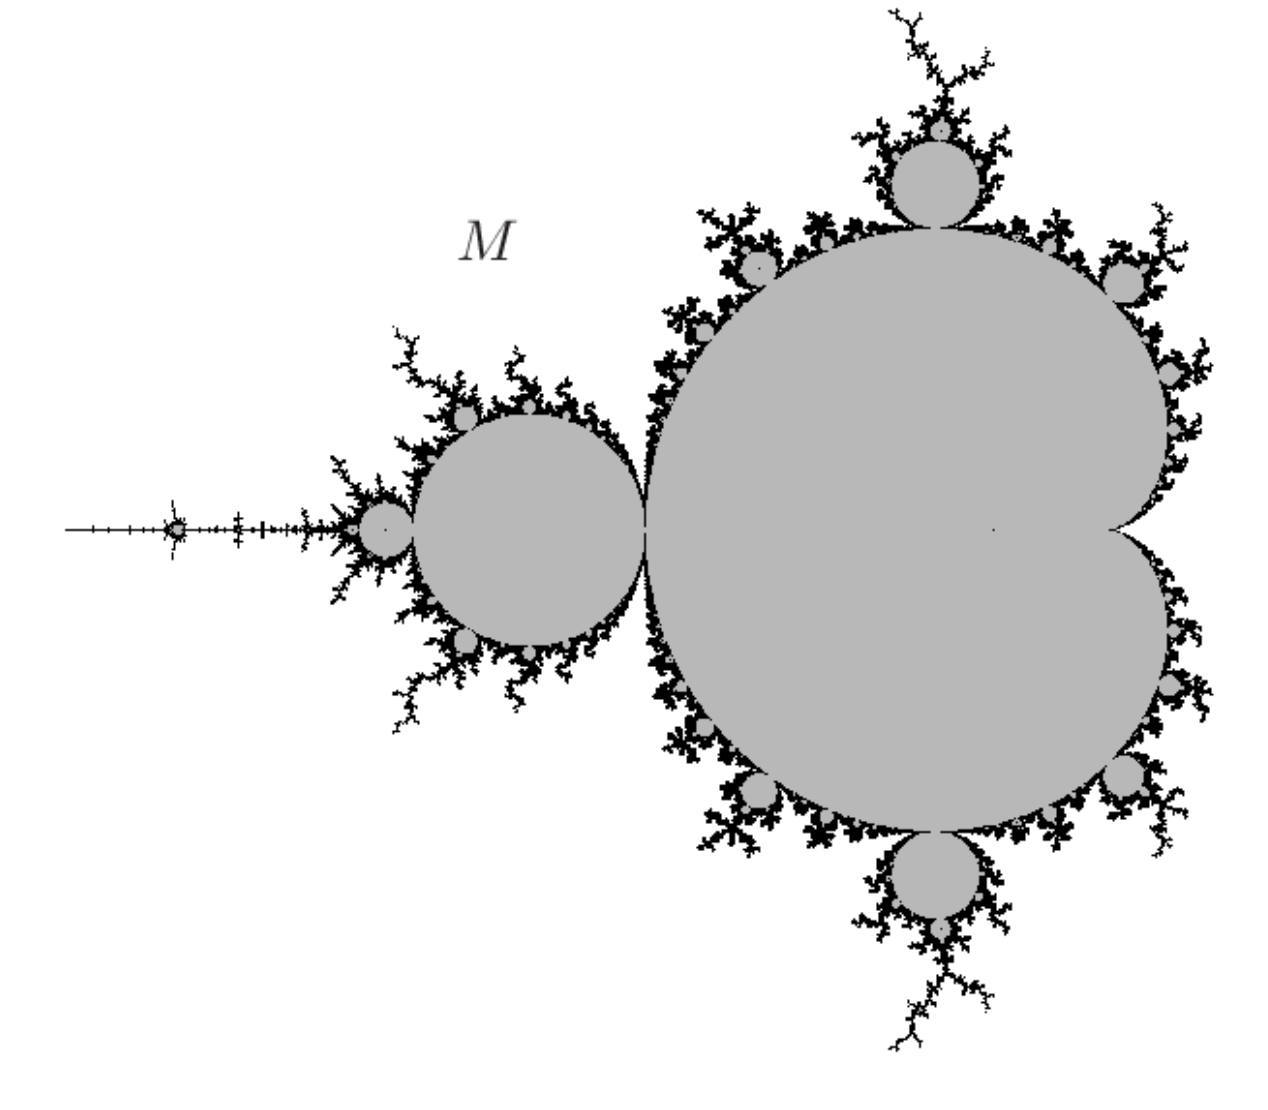
\includegraphics[width=0.65\textwidth]{mandelbrot}
\par}
\vspace{4mm}

It is known that for $c \notin \mathcal M$ the Julia set of $q_c$ is a Cantor set. Although $\mathcal M$ looks very complicated, it is connected.

\begin{theorem}
The Mandelbrot set is connected.
\end{theorem}
This was proved by Douady\footnote{Adrien Douady (1935--2006).} and Hubbard\footnote{John Hubbard (1945--).} in 1982 \cite{DH82}, \cite{DH85}. 
More recently, Shishikura\footnote{Mitsuhiro Shishikura (1960--).} showed that the Hausdorff dimension of the boundary of the Mandelbrot
set is equal to $2$ \cite{Shi98}.


There are two big open questions concerning the Mandelbrot set:\\

\noindent
\textbf{Conjectures:}\\
\noindent 1. The Mandelbrot set is  locally connected (i.e. given $c \in \mathcal M$ there is an open neighbourhood $U \subset \mathbb{C}$ containing $c$ such that $\mathcal M \cap U$ is connected).\\
\noindent 2. A point $c$ belongs to the interior of $\mathcal M$ if and only if $q_c$ has an attracting fixed point.\\

%Solving one of these conjectures would probably get you a Fields medal!\\


We finish the notes with some pictures of Julia sets. The following are Julia sets for the polynomials $z^2 + c$ for various values of $c$.

\vspace{4mm}
{\centering
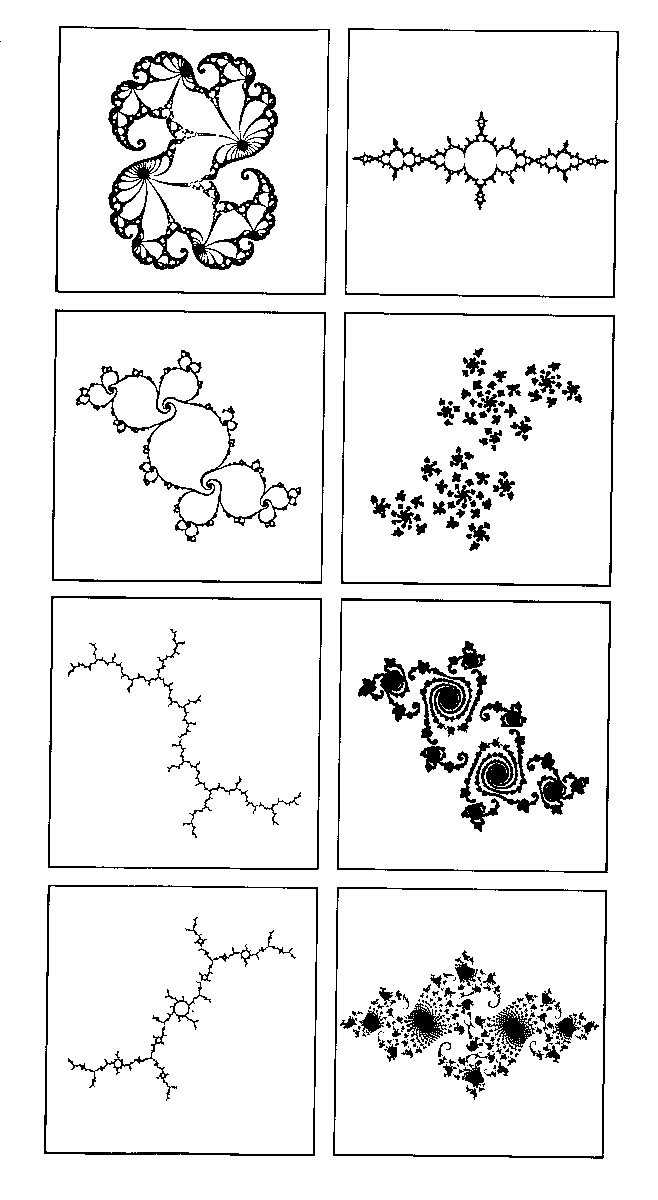
\includegraphics[width=0.65\textwidth]{juliasets} 
\par}

%\begin{proposition}
%Let $T$ be a hyperbolic toral automorphism of  $\mathbb R^{2}/\mathbb Z^{2}$ with
%corresponding matrix $A$ having eigenvalues $\lambda_{1},
%\lambda_{2}$.
%\begin{itemize}
%\item[(i)]
%The periodic points of $T$ correspond precisely with the set of
%rational points of $\mathbb R^{2}/\mathbb Z^{2}$:
%\[
% \left\{ \left( \frac{p_{1}}{q}, \frac{p_{2}}{q} \right) + \mathbb Z^{2} \mid
% p_{1},p_{2},q \in \mathbb N,\ 0 \leq p_{1},p_{2} < q \right\}.
%\]
%(In particular, the periodic points are dense.)
%\item[(ii)] 
%Suppose that $\det A = 1$.  Then the number of points of period $n$ is
%given by:
%\[
% \mathrm{card} \{ x \in \mathbb R^{2}/\mathbb Z^{2} \mid T^{n}(x)=x \} =
% | \lambda_{1}^{n} + \lambda_{2}^{n} -2 |.
%\]
%\end{itemize}
%\end{proposition}
%
%
%\begin{proof}
%A point $(x_{1},x_{2})$ is periodic with period $n$ for $T$ if and
%only if 
%\begin{equation}
%\label{eqn:noofperpts}
% (A^{n} -I)\left( \begin{array}{c} x_{1} \\ x_{2} \end{array} \right)
% = \left( \begin{array}{c} n_{1} \\ n_{2} \end{array} \right).
%\end{equation}
%We may take $x_{1},x_{2} \in [0,1)$.   Let $u = (A^{n}-I)(0,1), v =
%(A^{n}-I)(1,0)$.  The map $A^{n}-I$ maps
%$[0,1)\times[0,1)$ onto the parallelogram 
%\[
% R = \{ \alpha u + \beta v \mid 0 \leq \alpha, \beta < 1 \}.
%\]
%
%For the point $(x_{1}, x_{2}) \in [0,1) \times [0,1)$ to be periodic, it follows from
%(\ref{eqn:noofperpts}) that $(A^{n}-I)(x_{1}, x_{2})$ must be an
%integer point of $R$.  Thus the number of periodic points of period
%$n$ correspond to the number of integer points in $R$.  One can check
%that the number of such points is equal to the area of $R$.  Hence
%that number of periodic points of period $n$ is given by
%$|\det (A^{n}-I)|$.  
%
%
%Let us calculate the eigenvalues of $A^{n}-I$.  Let $\mu$ be an
%eigenvalue of $A^{n}-I$ with eigenvector $v$.  Then
%\[
% (A^{n}-I)v = \mu v  \Leftrightarrow  A^{n}v = (\mu+1)v
%\]
%so that $\mu+1$ is an eigenvalue of $A^{n}$.  As the eigenvalues of
%$A$ are given by $\lambda_{1}, \lambda_{2}$, the eigenvalues of
%$A^{n}$ are given by $\lambda_{1}^{n}, \lambda_{2}^{n}$.  Hence the
%eigenvalues of $A^{n}-I$ are $\lambda_{1}^{n}-1, \lambda_{2}^{n}-1$.
%As the determinant of a matrix is given by the product of the
%eigenvalues, we have that 
%\begin{eqnarray*}
% |\det (A^{n}-I)| & = & | (\lambda_{1}^{n}-1)(\lambda_{2}^{n}-1)| \\
% & = &
% |(\lambda_{1}\lambda_{2})^{n}+1 -(\lambda_{1}^{n}+\lambda_{2}^{n})| \\
% & = &
% \lambda_{1}^{n} + \lambda_{2}^{n} - 2,
%\end{eqnarray*}
%as $\lambda_{1}\lambda_{2} = \det A = 1$.
%\end{proof}






















%\newpage
%\section{Unimodal Interval Maps}

%\subsection{Introduction}









\newpage


\begin{thebibliography}{200000}

%\bibitem[AKM65]{AKM65}
%R. Adler, A. Konheim and M. McAndrew, Topological entropy, Trans. Amer. Math. Soc. 114, 309--319, %1965.

\bibitem[Ano67]{Anosov67}
D. Anosov, Geodesic flows on closed Riemannian manifolds with negative curvature,
Proc. Steklov Inst. Math. 90, 1967.

\bibitem[AA68]{AA68}
V. Arnold and A. Avez, Ergodic Problems of Classical Mechanics, Benjamin, New York, 1968.

\bibitem[Bea91]{Bea91}
A. Beardon, Iteration of Rational Functions. Complex Analytical Dynamical Systems, 
Graduate Texts in Mathematics 132, Springer--Verlag, New York, 1991.

%\bibitem[Bow70]{Bow70}
%R. Bowen, Markov partitions for Axion A diffeomorphisms, Amer. J. Math. 92, 725--747, 1970.

%\bibitem[Bow71]{Bow71}
%R. Bowen, Entropy for group endomorphisms and homogeneous spaces,
%Trans. Amer. Math. Soc. 153, 401--414, 1971.

\bibitem[BS02]{BS02}
M. Brin and G. Stuck, Introduction to Dynamical Systems, Cambridge University Press, Cambridge,
2002.

\bibitem[BM78]{BM78}
R. Brooks and J. Matelski, The dynamics of $2$-generator subgroups of $\mathrm{PSL}(2,\mathbf C)$,
Riemann Surfaces  and Related Topics: Proceedings of the 1978 Stony Brook Conference,
Princeton University Press, 1980.

\bibitem[Dev03]{Dev03}
R. Devany, An Introduction to Chaotic Dynamical Systems (second edition),
Westview Press, Boulder, Colorado, 2003.

%\bibitem[Din70]{Dinaburg}
%E. Dinaburg, The relation between topological entropy and metric entropy,
%Soviet Math. 11, 13--16, 1970.

\bibitem[DH82]{DH82}
A. Douady and J. Hubbard,
It\'eration des polyn\^omes quadratiques complexes, Comptes Rendus Acad. Sci. Paris 294, 123--126, 1982.

\bibitem[DH85]{DH85}
A. Douady and J. Hubbard,
On the dynamics of polynomial-like mappings, Ann. Sci. \'Ecole Normale
Sup\'erieure 18, 287--343, 1985.

\bibitem[HK03]{HK03}
B. Hasselblatt and A. Katok, A First Course in Dynamical Systems,
Cambridge University Press, Cambridge,
2003.

\bibitem[KH95]{KH95}
A. Katok and B. Hasselblatt, Introduction to the Modern Theory of Dynamical
Systems, Cambridge University Press, Cambridge,
1995.

%\bibitem[Man71]{Man71}
%A. Manning, Axiom A diffeomorphisms have rational zeta functions,
%Bull. London Math. Soc. 3, 215--220, 1971.


%\bibitem[Rob99]{Robinson}
%C. Robinson, Dynamical Systems: Stability, Symbolic Dynamics and Chaos, CRC Press,
%Boca Raton--London--New York--Washington DC,
%1998.

\bibitem[Shi98]{Shi98}
M. Shishikura,
The Hausdorff dimension of the boundary of the Mandelbrot set and Julia sets,
Annals of Math. 147, 225--267, 1998.

%\bibitem[Shu87]{Shu87}
%M. Shub, Global Stability of Dynamical Systems, Springer--Verlag, New York--Heidelberg--Berlin, 1987.

\bibitem[Sma67]{Smale67}
S. Smale, Differentiable dynamical systems, Bull. Amer. Math. Soc. 73,
747--817, 1967.

\bibitem[Stein93]{Stein93}
N. Steinmetz, Rational Iteration. Complex Analytic Dynamical Systems,
De Gruyter Studies in Mathematics 16, Walter de Gruyter \& Co., Berlin, 1993.

\bibitem[Ste10]{Ste10}
S. Sternberg, Dynamical Systems, Dover, Mineola, New York, 2010.

%\bibitem[Wal76]{Walters76}
%P. Walters, A variational principle for the pressure of continuous transformations,
%Amer. J. Math. 17, 937--971, 1976.

\bibitem[Wal82]{Walters}
P.~Walters,
\newblock An Introduction to Ergodic Theory,
\newblock Graduate Texts in Mathematics 79, Springer--Verlag, New York--Heidelberg--Berlin, 1982.


\end{thebibliography}

\end{document}









